\documentclass[twoside]{book}

% Packages required by doxygen
\usepackage{calc}
\usepackage{doxygen}
\usepackage{graphicx}
\usepackage[utf8]{inputenc}
\usepackage{makeidx}
\usepackage{multicol}
\usepackage{multirow}
\usepackage{textcomp}
\usepackage[table]{xcolor}

% Font selection
\usepackage[T1]{fontenc}
\usepackage{mathptmx}
\usepackage[scaled=.90]{helvet}
\usepackage{courier}
\usepackage{amssymb}
\usepackage{sectsty}
\renewcommand{\familydefault}{\sfdefault}
\allsectionsfont{%
  \fontseries{bc}\selectfont%
  \color{darkgray}%
}
\renewcommand{\DoxyLabelFont}{%
  \fontseries{bc}\selectfont%
  \color{darkgray}%
}

% Page & text layout
\usepackage{geometry}
\geometry{%
  a4paper,%
  top=2.5cm,%
  bottom=2.5cm,%
  left=2.5cm,%
  right=2.5cm%
}
\tolerance=750
\hfuzz=15pt
\hbadness=750
\setlength{\emergencystretch}{15pt}
\setlength{\parindent}{0cm}
\setlength{\parskip}{0.2cm}
\makeatletter
\renewcommand{\paragraph}{%
  \@startsection{paragraph}{4}{0ex}{-1.0ex}{1.0ex}{%
    \normalfont\normalsize\bfseries\SS@parafont%
  }%
}
\renewcommand{\subparagraph}{%
  \@startsection{subparagraph}{5}{0ex}{-1.0ex}{1.0ex}{%
    \normalfont\normalsize\bfseries\SS@subparafont%
  }%
}
\makeatother

% Headers & footers
\usepackage{fancyhdr}
\pagestyle{fancyplain}
\fancyhead[LE]{\fancyplain{}{\bfseries\thepage}}
\fancyhead[CE]{\fancyplain{}{}}
\fancyhead[RE]{\fancyplain{}{\bfseries\leftmark}}
\fancyhead[LO]{\fancyplain{}{\bfseries\rightmark}}
\fancyhead[CO]{\fancyplain{}{}}
\fancyhead[RO]{\fancyplain{}{\bfseries\thepage}}
\fancyfoot[LE]{\fancyplain{}{}}
\fancyfoot[CE]{\fancyplain{}{}}
\fancyfoot[RE]{\fancyplain{}{\bfseries\scriptsize Generated on Thu Nov 19 2015 21\-:26\-:36 for My Project by Doxygen }}
\fancyfoot[LO]{\fancyplain{}{\bfseries\scriptsize Generated on Thu Nov 19 2015 21\-:26\-:36 for My Project by Doxygen }}
\fancyfoot[CO]{\fancyplain{}{}}
\fancyfoot[RO]{\fancyplain{}{}}
\renewcommand{\footrulewidth}{0.4pt}
\renewcommand{\chaptermark}[1]{%
  \markboth{#1}{}%
}
\renewcommand{\sectionmark}[1]{%
  \markright{\thesection\ #1}%
}

% Indices & bibliography
\usepackage{natbib}
\usepackage[titles]{tocloft}
\setcounter{tocdepth}{3}
\setcounter{secnumdepth}{5}
\makeindex

% Hyperlinks (required, but should be loaded last)
\usepackage{ifpdf}
\ifpdf
  \usepackage[pdftex,pagebackref=true]{hyperref}
\else
  \usepackage[ps2pdf,pagebackref=true]{hyperref}
\fi
\hypersetup{%
  colorlinks=true,%
  linkcolor=blue,%
  citecolor=blue,%
  unicode%
}

% Custom commands
\newcommand{\clearemptydoublepage}{%
  \newpage{\pagestyle{empty}\cleardoublepage}%
}


%===== C O N T E N T S =====

\begin{document}

% Titlepage & ToC
\hypersetup{pageanchor=false}
\pagenumbering{roman}
\begin{titlepage}
\vspace*{7cm}
\begin{center}%
{\Large My Project }\\
\vspace*{1cm}
{\large Generated by Doxygen 1.8.6}\\
\vspace*{0.5cm}
{\small Thu Nov 19 2015 21:26:36}\\
\end{center}
\end{titlepage}
\clearemptydoublepage
\tableofcontents
\clearemptydoublepage
\pagenumbering{arabic}
\hypersetup{pageanchor=true}

%--- Begin generated contents ---
\chapter{cs371p-\/life}
\label{md_README}
\hypertarget{md_README}{}
\input{md_README}
\chapter{Hierarchical Index}
\section{Class Hierarchy}
This inheritance list is sorted roughly, but not completely, alphabetically\-:\begin{DoxyCompactList}
\item \contentsline{section}{Abstract\-Cell}{\pageref{classAbstractCell}}{}
\begin{DoxyCompactList}
\item \contentsline{section}{Conway\-Cell}{\pageref{classConwayCell}}{}
\item \contentsline{section}{Fredkin\-Cell}{\pageref{classFredkinCell}}{}
\end{DoxyCompactList}
\item \contentsline{section}{Cell}{\pageref{classCell}}{}
\item \contentsline{section}{L\-\_\-\-Iterator$<$ T $>$}{\pageref{classL__Iterator}}{}
\item \contentsline{section}{Life$<$ T $>$}{\pageref{classLife}}{}
\end{DoxyCompactList}

\chapter{Class Index}
\section{Class List}
Here are the classes, structs, unions and interfaces with brief descriptions\-:\begin{DoxyCompactList}
\item\contentsline{section}{\hyperlink{classAbstractCell}{Abstract\-Cell} }{\pageref{classAbstractCell}}{}
\item\contentsline{section}{\hyperlink{classCell}{Cell} }{\pageref{classCell}}{}
\item\contentsline{section}{\hyperlink{classConwayCell}{Conway\-Cell} }{\pageref{classConwayCell}}{}
\item\contentsline{section}{\hyperlink{classFredkinCell}{Fredkin\-Cell} }{\pageref{classFredkinCell}}{}
\item\contentsline{section}{\hyperlink{classL__Iterator}{L\-\_\-\-Iterator$<$ T $>$} }{\pageref{classL__Iterator}}{}
\item\contentsline{section}{\hyperlink{classLife}{Life$<$ T $>$} }{\pageref{classLife}}{}
\end{DoxyCompactList}

\chapter{File Index}
\section{File List}
Here is a list of all files with brief descriptions\-:\begin{DoxyCompactList}
\item\contentsline{section}{\hyperlink{Life_8c_09_09}{Life.\-c++} }{\pageref{Life_8c_09_09}}{}
\item\contentsline{section}{\hyperlink{Life_8h}{Life.\-h} }{\pageref{Life_8h}}{}
\item\contentsline{section}{\hyperlink{LifeTestMaker_8c_09_09}{Life\-Test\-Maker.\-c++} }{\pageref{LifeTestMaker_8c_09_09}}{}
\item\contentsline{section}{\hyperlink{RunLife_8c_09_09}{Run\-Life.\-c++} }{\pageref{RunLife_8c_09_09}}{}
\item\contentsline{section}{\hyperlink{TestLife_8c_09_09}{Test\-Life.\-c++} }{\pageref{TestLife_8c_09_09}}{}
\end{DoxyCompactList}

\chapter{Class Documentation}
\hypertarget{classAbstractCell}{\section{Abstract\-Cell Class Reference}
\label{classAbstractCell}\index{Abstract\-Cell@{Abstract\-Cell}}
}


{\ttfamily \#include $<$Life.\-h$>$}

Inheritance diagram for Abstract\-Cell\-:\begin{figure}[H]
\begin{center}
\leavevmode
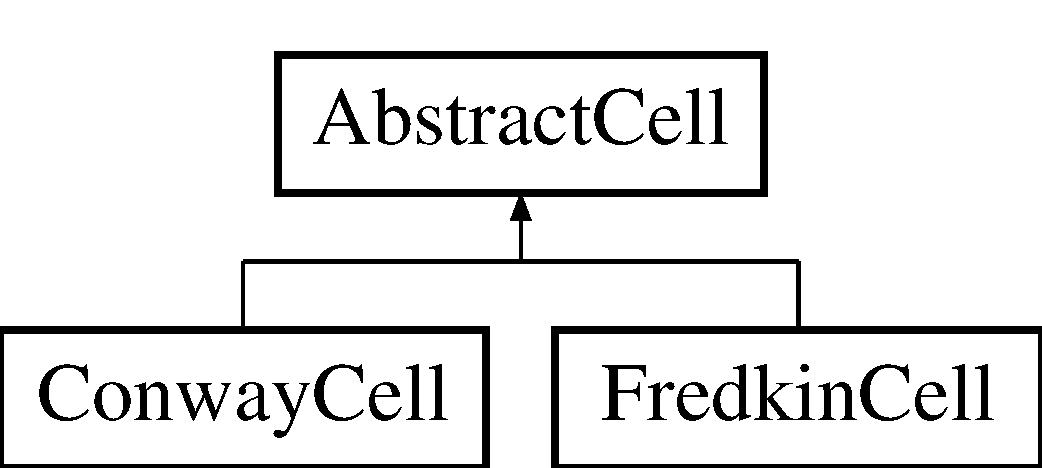
\includegraphics[height=2.000000cm]{classAbstractCell}
\end{center}
\end{figure}
\subsection*{Public Member Functions}
\begin{DoxyCompactItemize}
\item 
virtual \hyperlink{classAbstractCell_a4576179f57220c4342edd9b01563df63}{$\sim$\-Abstract\-Cell} ()
\item 
virtual \hyperlink{classAbstractCell}{Abstract\-Cell} $\ast$ \hyperlink{classAbstractCell_a1a95a7ea92b3503e2f042170b6320354}{clone} () const =0
\item 
virtual void \hyperlink{classAbstractCell_a3400569dbc73b019698bead4aca5b186}{evolve} (int, \hyperlink{classLife}{Life}$<$ \hyperlink{classCell}{Cell} $>$ \&)=0
\item 
virtual bool \hyperlink{classAbstractCell_ad19a847847061bcbe642932ba34713b3}{can\-Mutate} ()
\item 
virtual int \hyperlink{classAbstractCell_a86553456ecaaeb0d7e94b92e123540b6}{change\-State} ()
\item 
virtual int \hyperlink{classAbstractCell_ac4bba10e2bc5da7fe5c601d04c75821f}{is\-Alive} (int count)
\end{DoxyCompactItemize}
\subsection*{Protected Attributes}
\begin{DoxyCompactItemize}
\item 
bool \hyperlink{classAbstractCell_a738a87fd7a98a0bbeb723d0690b07e97}{current\-\_\-state} = false
\item 
bool \hyperlink{classAbstractCell_a196b0194fb5cd8701b0aae28d12a0586}{next\-\_\-state} = false
\item 
char \hyperlink{classAbstractCell_ad763295e814970b07d31d98b560a4b19}{symbol} = ' '
\item 
int \hyperlink{classAbstractCell_a99e95bd6e878d85cb33a9fe90c4b7d25}{age} = 0
\end{DoxyCompactItemize}
\subsection*{Friends}
\begin{DoxyCompactItemize}
\item 
std\-::ostream \& \hyperlink{classAbstractCell_abe6e58e7a719ee8f4a34181ccca158a2}{operator$<$$<$} (std\-::ostream \&, const \hyperlink{classCell}{Cell} \&)
\end{DoxyCompactItemize}


\subsection{Constructor \& Destructor Documentation}
\hypertarget{classAbstractCell_a4576179f57220c4342edd9b01563df63}{\index{Abstract\-Cell@{Abstract\-Cell}!$\sim$\-Abstract\-Cell@{$\sim$\-Abstract\-Cell}}
\index{$\sim$\-Abstract\-Cell@{$\sim$\-Abstract\-Cell}!AbstractCell@{Abstract\-Cell}}
\subsubsection[{$\sim$\-Abstract\-Cell}]{\setlength{\rightskip}{0pt plus 5cm}virtual Abstract\-Cell\-::$\sim$\-Abstract\-Cell (
\begin{DoxyParamCaption}
{}
\end{DoxyParamCaption}
)\hspace{0.3cm}{\ttfamily [inline]}, {\ttfamily [virtual]}}}\label{classAbstractCell_a4576179f57220c4342edd9b01563df63}


\subsection{Member Function Documentation}
\hypertarget{classAbstractCell_ad19a847847061bcbe642932ba34713b3}{\index{Abstract\-Cell@{Abstract\-Cell}!can\-Mutate@{can\-Mutate}}
\index{can\-Mutate@{can\-Mutate}!AbstractCell@{Abstract\-Cell}}
\subsubsection[{can\-Mutate}]{\setlength{\rightskip}{0pt plus 5cm}virtual bool Abstract\-Cell\-::can\-Mutate (
\begin{DoxyParamCaption}
{}
\end{DoxyParamCaption}
)\hspace{0.3cm}{\ttfamily [inline]}, {\ttfamily [virtual]}}}\label{classAbstractCell_ad19a847847061bcbe642932ba34713b3}
\hypertarget{classAbstractCell_a86553456ecaaeb0d7e94b92e123540b6}{\index{Abstract\-Cell@{Abstract\-Cell}!change\-State@{change\-State}}
\index{change\-State@{change\-State}!AbstractCell@{Abstract\-Cell}}
\subsubsection[{change\-State}]{\setlength{\rightskip}{0pt plus 5cm}virtual int Abstract\-Cell\-::change\-State (
\begin{DoxyParamCaption}
{}
\end{DoxyParamCaption}
)\hspace{0.3cm}{\ttfamily [inline]}, {\ttfamily [virtual]}}}\label{classAbstractCell_a86553456ecaaeb0d7e94b92e123540b6}
\hypertarget{classAbstractCell_a1a95a7ea92b3503e2f042170b6320354}{\index{Abstract\-Cell@{Abstract\-Cell}!clone@{clone}}
\index{clone@{clone}!AbstractCell@{Abstract\-Cell}}
\subsubsection[{clone}]{\setlength{\rightskip}{0pt plus 5cm}virtual {\bf Abstract\-Cell}$\ast$ Abstract\-Cell\-::clone (
\begin{DoxyParamCaption}
{}
\end{DoxyParamCaption}
) const\hspace{0.3cm}{\ttfamily [pure virtual]}}}\label{classAbstractCell_a1a95a7ea92b3503e2f042170b6320354}


Implemented in \hyperlink{classFredkinCell_a05d7cd1308b23d514e207317fdf06235}{Fredkin\-Cell}, and \hyperlink{classConwayCell_a0fac73dc33d36053d1400430f1c980ce}{Conway\-Cell}.

\hypertarget{classAbstractCell_a3400569dbc73b019698bead4aca5b186}{\index{Abstract\-Cell@{Abstract\-Cell}!evolve@{evolve}}
\index{evolve@{evolve}!AbstractCell@{Abstract\-Cell}}
\subsubsection[{evolve}]{\setlength{\rightskip}{0pt plus 5cm}virtual void Abstract\-Cell\-::evolve (
\begin{DoxyParamCaption}
\item[{int}]{, }
\item[{{\bf Life}$<$ {\bf Cell} $>$ \&}]{}
\end{DoxyParamCaption}
)\hspace{0.3cm}{\ttfamily [pure virtual]}}}\label{classAbstractCell_a3400569dbc73b019698bead4aca5b186}


Implemented in \hyperlink{classFredkinCell_a662b6ad6a17cda14b4563a17c6ae4eed}{Fredkin\-Cell}, and \hyperlink{classConwayCell_ad7204969de71ae212c67b5eafcd333f0}{Conway\-Cell}.

\hypertarget{classAbstractCell_ac4bba10e2bc5da7fe5c601d04c75821f}{\index{Abstract\-Cell@{Abstract\-Cell}!is\-Alive@{is\-Alive}}
\index{is\-Alive@{is\-Alive}!AbstractCell@{Abstract\-Cell}}
\subsubsection[{is\-Alive}]{\setlength{\rightskip}{0pt plus 5cm}virtual int Abstract\-Cell\-::is\-Alive (
\begin{DoxyParamCaption}
\item[{int}]{count}
\end{DoxyParamCaption}
)\hspace{0.3cm}{\ttfamily [inline]}, {\ttfamily [virtual]}}}\label{classAbstractCell_ac4bba10e2bc5da7fe5c601d04c75821f}


\subsection{Friends And Related Function Documentation}
\hypertarget{classAbstractCell_abe6e58e7a719ee8f4a34181ccca158a2}{\index{Abstract\-Cell@{Abstract\-Cell}!operator$<$$<$@{operator$<$$<$}}
\index{operator$<$$<$@{operator$<$$<$}!AbstractCell@{Abstract\-Cell}}
\subsubsection[{operator$<$$<$}]{\setlength{\rightskip}{0pt plus 5cm}std\-::ostream\& operator$<$$<$ (
\begin{DoxyParamCaption}
\item[{std\-::ostream \&}]{, }
\item[{const {\bf Cell} \&}]{}
\end{DoxyParamCaption}
)\hspace{0.3cm}{\ttfamily [friend]}}}\label{classAbstractCell_abe6e58e7a719ee8f4a34181ccca158a2}


\subsection{Member Data Documentation}
\hypertarget{classAbstractCell_a99e95bd6e878d85cb33a9fe90c4b7d25}{\index{Abstract\-Cell@{Abstract\-Cell}!age@{age}}
\index{age@{age}!AbstractCell@{Abstract\-Cell}}
\subsubsection[{age}]{\setlength{\rightskip}{0pt plus 5cm}int Abstract\-Cell\-::age = 0\hspace{0.3cm}{\ttfamily [protected]}}}\label{classAbstractCell_a99e95bd6e878d85cb33a9fe90c4b7d25}
\hypertarget{classAbstractCell_a738a87fd7a98a0bbeb723d0690b07e97}{\index{Abstract\-Cell@{Abstract\-Cell}!current\-\_\-state@{current\-\_\-state}}
\index{current\-\_\-state@{current\-\_\-state}!AbstractCell@{Abstract\-Cell}}
\subsubsection[{current\-\_\-state}]{\setlength{\rightskip}{0pt plus 5cm}bool Abstract\-Cell\-::current\-\_\-state = false\hspace{0.3cm}{\ttfamily [protected]}}}\label{classAbstractCell_a738a87fd7a98a0bbeb723d0690b07e97}
\hypertarget{classAbstractCell_a196b0194fb5cd8701b0aae28d12a0586}{\index{Abstract\-Cell@{Abstract\-Cell}!next\-\_\-state@{next\-\_\-state}}
\index{next\-\_\-state@{next\-\_\-state}!AbstractCell@{Abstract\-Cell}}
\subsubsection[{next\-\_\-state}]{\setlength{\rightskip}{0pt plus 5cm}bool Abstract\-Cell\-::next\-\_\-state = false\hspace{0.3cm}{\ttfamily [protected]}}}\label{classAbstractCell_a196b0194fb5cd8701b0aae28d12a0586}
\hypertarget{classAbstractCell_ad763295e814970b07d31d98b560a4b19}{\index{Abstract\-Cell@{Abstract\-Cell}!symbol@{symbol}}
\index{symbol@{symbol}!AbstractCell@{Abstract\-Cell}}
\subsubsection[{symbol}]{\setlength{\rightskip}{0pt plus 5cm}char Abstract\-Cell\-::symbol = ' '\hspace{0.3cm}{\ttfamily [protected]}}}\label{classAbstractCell_ad763295e814970b07d31d98b560a4b19}


The documentation for this class was generated from the following file\-:\begin{DoxyCompactItemize}
\item 
\hyperlink{Life_8h}{Life.\-h}\end{DoxyCompactItemize}

\hypertarget{classCell}{\section{Cell Class Reference}
\label{classCell}\index{Cell@{Cell}}
}


{\ttfamily \#include $<$Life.\-h$>$}

\subsection*{Public Member Functions}
\begin{DoxyCompactItemize}
\item 
\hyperlink{classCell_a394510643e8664cf12b5efaf5cb99f71}{Cell} ()
\item 
\hyperlink{classCell_a05a40af833aa8976b67a109385bd3cb0}{Cell} (const \hyperlink{classAbstractCell}{Abstract\-Cell} $\ast$)
\item 
\hyperlink{classCell_a4f4f93a1878d4dd7bac8f7df6629068b}{Cell} (bool, char)
\item 
void \hyperlink{classCell_a956383653c570c0b085752c2a9bdd89c}{operator=} (const \hyperlink{classCell}{Cell} \&)
\item 
void \hyperlink{classCell_aeefadf6295020f9cbfb52d50a3721b2c}{evolve} (int, \hyperlink{classLife}{Life}$<$ \hyperlink{classCell}{Cell} $>$ \&)
\item 
bool \hyperlink{classCell_a63bbde8923e149c01d5ef6e3e9492a97}{can\-Mutate} ()
\item 
int \hyperlink{classCell_ac372cb0291cec89407f82ad3c306513a}{change\-State} ()
\item 
int \hyperlink{classCell_a508e59acbfa9e14d327246238c7cc181}{is\-Alive} (int)
\end{DoxyCompactItemize}
\subsection*{Private Attributes}
\begin{DoxyCompactItemize}
\item 
\hyperlink{classAbstractCell}{Abstract\-Cell} $\ast$ \hyperlink{classCell_ac51b82d0179572d599b7837e4df90e4d}{ac\-\_\-ptr}
\end{DoxyCompactItemize}
\subsection*{Friends}
\begin{DoxyCompactItemize}
\item 
std\-::ostream \& \hyperlink{classCell_abe6e58e7a719ee8f4a34181ccca158a2}{operator$<$$<$} (std\-::ostream \&, const \hyperlink{classCell}{Cell} \&)
\end{DoxyCompactItemize}


\subsection{Constructor \& Destructor Documentation}
\hypertarget{classCell_a394510643e8664cf12b5efaf5cb99f71}{\index{Cell@{Cell}!Cell@{Cell}}
\index{Cell@{Cell}!Cell@{Cell}}
\subsubsection[{Cell}]{\setlength{\rightskip}{0pt plus 5cm}Cell\-::\-Cell (
\begin{DoxyParamCaption}
{}
\end{DoxyParamCaption}
)}}\label{classCell_a394510643e8664cf12b5efaf5cb99f71}
\hypertarget{classCell_a05a40af833aa8976b67a109385bd3cb0}{\index{Cell@{Cell}!Cell@{Cell}}
\index{Cell@{Cell}!Cell@{Cell}}
\subsubsection[{Cell}]{\setlength{\rightskip}{0pt plus 5cm}Cell\-::\-Cell (
\begin{DoxyParamCaption}
\item[{const {\bf Abstract\-Cell} $\ast$}]{ac}
\end{DoxyParamCaption}
)}}\label{classCell_a05a40af833aa8976b67a109385bd3cb0}
\hypertarget{classCell_a4f4f93a1878d4dd7bac8f7df6629068b}{\index{Cell@{Cell}!Cell@{Cell}}
\index{Cell@{Cell}!Cell@{Cell}}
\subsubsection[{Cell}]{\setlength{\rightskip}{0pt plus 5cm}Cell\-::\-Cell (
\begin{DoxyParamCaption}
\item[{bool}]{initial\-\_\-state, }
\item[{char}]{s}
\end{DoxyParamCaption}
)}}\label{classCell_a4f4f93a1878d4dd7bac8f7df6629068b}


\subsection{Member Function Documentation}
\hypertarget{classCell_a63bbde8923e149c01d5ef6e3e9492a97}{\index{Cell@{Cell}!can\-Mutate@{can\-Mutate}}
\index{can\-Mutate@{can\-Mutate}!Cell@{Cell}}
\subsubsection[{can\-Mutate}]{\setlength{\rightskip}{0pt plus 5cm}bool Cell\-::can\-Mutate (
\begin{DoxyParamCaption}
{}
\end{DoxyParamCaption}
)}}\label{classCell_a63bbde8923e149c01d5ef6e3e9492a97}
\hypertarget{classCell_ac372cb0291cec89407f82ad3c306513a}{\index{Cell@{Cell}!change\-State@{change\-State}}
\index{change\-State@{change\-State}!Cell@{Cell}}
\subsubsection[{change\-State}]{\setlength{\rightskip}{0pt plus 5cm}int Cell\-::change\-State (
\begin{DoxyParamCaption}
{}
\end{DoxyParamCaption}
)}}\label{classCell_ac372cb0291cec89407f82ad3c306513a}
\hypertarget{classCell_aeefadf6295020f9cbfb52d50a3721b2c}{\index{Cell@{Cell}!evolve@{evolve}}
\index{evolve@{evolve}!Cell@{Cell}}
\subsubsection[{evolve}]{\setlength{\rightskip}{0pt plus 5cm}void Cell\-::evolve (
\begin{DoxyParamCaption}
\item[{int}]{index, }
\item[{{\bf Life}$<$ {\bf Cell} $>$ \&}]{l}
\end{DoxyParamCaption}
)}}\label{classCell_aeefadf6295020f9cbfb52d50a3721b2c}
\hypertarget{classCell_a508e59acbfa9e14d327246238c7cc181}{\index{Cell@{Cell}!is\-Alive@{is\-Alive}}
\index{is\-Alive@{is\-Alive}!Cell@{Cell}}
\subsubsection[{is\-Alive}]{\setlength{\rightskip}{0pt plus 5cm}int Cell\-::is\-Alive (
\begin{DoxyParamCaption}
\item[{int}]{count}
\end{DoxyParamCaption}
)}}\label{classCell_a508e59acbfa9e14d327246238c7cc181}
\hypertarget{classCell_a956383653c570c0b085752c2a9bdd89c}{\index{Cell@{Cell}!operator=@{operator=}}
\index{operator=@{operator=}!Cell@{Cell}}
\subsubsection[{operator=}]{\setlength{\rightskip}{0pt plus 5cm}void Cell\-::operator= (
\begin{DoxyParamCaption}
\item[{const {\bf Cell} \&}]{c}
\end{DoxyParamCaption}
)}}\label{classCell_a956383653c570c0b085752c2a9bdd89c}


\subsection{Friends And Related Function Documentation}
\hypertarget{classCell_abe6e58e7a719ee8f4a34181ccca158a2}{\index{Cell@{Cell}!operator$<$$<$@{operator$<$$<$}}
\index{operator$<$$<$@{operator$<$$<$}!Cell@{Cell}}
\subsubsection[{operator$<$$<$}]{\setlength{\rightskip}{0pt plus 5cm}std\-::ostream\& operator$<$$<$ (
\begin{DoxyParamCaption}
\item[{std\-::ostream \&}]{, }
\item[{const {\bf Cell} \&}]{}
\end{DoxyParamCaption}
)\hspace{0.3cm}{\ttfamily [friend]}}}\label{classCell_abe6e58e7a719ee8f4a34181ccca158a2}


\subsection{Member Data Documentation}
\hypertarget{classCell_ac51b82d0179572d599b7837e4df90e4d}{\index{Cell@{Cell}!ac\-\_\-ptr@{ac\-\_\-ptr}}
\index{ac\-\_\-ptr@{ac\-\_\-ptr}!Cell@{Cell}}
\subsubsection[{ac\-\_\-ptr}]{\setlength{\rightskip}{0pt plus 5cm}{\bf Abstract\-Cell}$\ast$ Cell\-::ac\-\_\-ptr\hspace{0.3cm}{\ttfamily [private]}}}\label{classCell_ac51b82d0179572d599b7837e4df90e4d}


The documentation for this class was generated from the following files\-:\begin{DoxyCompactItemize}
\item 
\hyperlink{Life_8h}{Life.\-h}\item 
\hyperlink{Life_8c_09_09}{Life.\-c++}\end{DoxyCompactItemize}

\hypertarget{classConwayCell}{\section{Conway\-Cell Class Reference}
\label{classConwayCell}\index{Conway\-Cell@{Conway\-Cell}}
}


{\ttfamily \#include $<$Life.\-h$>$}

Inheritance diagram for Conway\-Cell\-:\begin{figure}[H]
\begin{center}
\leavevmode
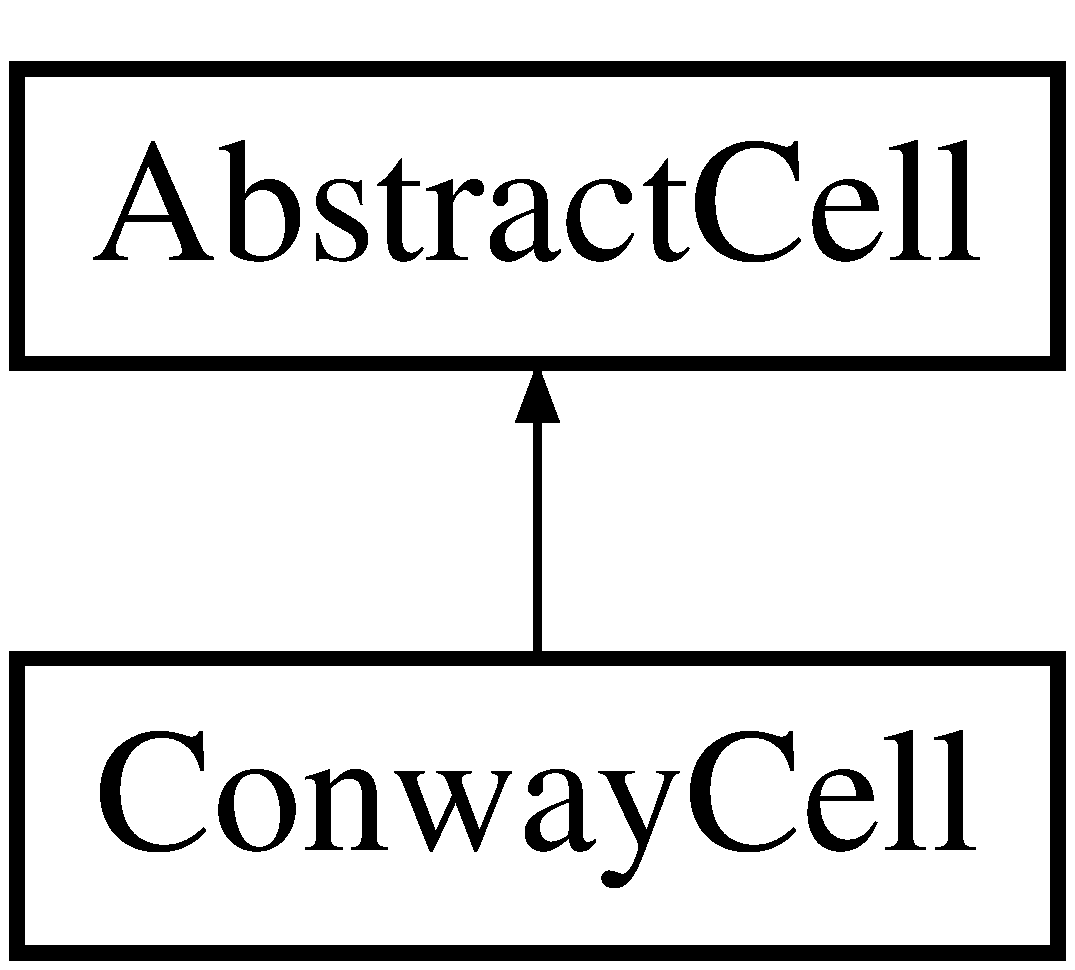
\includegraphics[height=2.000000cm]{classConwayCell}
\end{center}
\end{figure}
\subsection*{Public Member Functions}
\begin{DoxyCompactItemize}
\item 
\hyperlink{classConwayCell_aeff597ba7adcb28d4c386d075eddb196}{Conway\-Cell} ()
\item 
\hyperlink{classConwayCell_a2a95bc5f44490fcc91e40b6a5c98ab86}{Conway\-Cell} (\hyperlink{classAbstractCell}{Abstract\-Cell} $\ast$)
\item 
\hyperlink{classConwayCell_a5a3c45dac7c4de6119fb9d0dfdfab710}{Conway\-Cell} (bool, char)
\item 
\hyperlink{classConwayCell}{Conway\-Cell} $\ast$ \hyperlink{classConwayCell_a0fac73dc33d36053d1400430f1c980ce}{clone} () const 
\item 
void \hyperlink{classConwayCell_af5de668c6c40874a915da6335e030aa6}{evolve} (int, \hyperlink{classLife}{Life}$<$ \hyperlink{classConwayCell}{Conway\-Cell} $>$ \&)
\item 
void \hyperlink{classConwayCell_ad7204969de71ae212c67b5eafcd333f0}{evolve} (int, \hyperlink{classLife}{Life}$<$ \hyperlink{classCell}{Cell} $>$ \&)
\end{DoxyCompactItemize}
\subsection*{Friends}
\begin{DoxyCompactItemize}
\item 
std\-::ostream \& \hyperlink{classConwayCell_a30841fd52a1b9f1980a5e3345d7c6b9f}{operator$<$$<$} (std\-::ostream \&, const \hyperlink{classConwayCell}{Conway\-Cell} \&)
\end{DoxyCompactItemize}
\subsection*{Additional Inherited Members}


\subsection{Constructor \& Destructor Documentation}
\hypertarget{classConwayCell_aeff597ba7adcb28d4c386d075eddb196}{\index{Conway\-Cell@{Conway\-Cell}!Conway\-Cell@{Conway\-Cell}}
\index{Conway\-Cell@{Conway\-Cell}!ConwayCell@{Conway\-Cell}}
\subsubsection[{Conway\-Cell}]{\setlength{\rightskip}{0pt plus 5cm}Conway\-Cell\-::\-Conway\-Cell (
\begin{DoxyParamCaption}
{}
\end{DoxyParamCaption}
)}}\label{classConwayCell_aeff597ba7adcb28d4c386d075eddb196}
\hypertarget{classConwayCell_a2a95bc5f44490fcc91e40b6a5c98ab86}{\index{Conway\-Cell@{Conway\-Cell}!Conway\-Cell@{Conway\-Cell}}
\index{Conway\-Cell@{Conway\-Cell}!ConwayCell@{Conway\-Cell}}
\subsubsection[{Conway\-Cell}]{\setlength{\rightskip}{0pt plus 5cm}Conway\-Cell\-::\-Conway\-Cell (
\begin{DoxyParamCaption}
\item[{{\bf Abstract\-Cell} $\ast$}]{}
\end{DoxyParamCaption}
)}}\label{classConwayCell_a2a95bc5f44490fcc91e40b6a5c98ab86}
\hypertarget{classConwayCell_a5a3c45dac7c4de6119fb9d0dfdfab710}{\index{Conway\-Cell@{Conway\-Cell}!Conway\-Cell@{Conway\-Cell}}
\index{Conway\-Cell@{Conway\-Cell}!ConwayCell@{Conway\-Cell}}
\subsubsection[{Conway\-Cell}]{\setlength{\rightskip}{0pt plus 5cm}Conway\-Cell\-::\-Conway\-Cell (
\begin{DoxyParamCaption}
\item[{bool}]{initial\-\_\-state, }
\item[{char}]{s}
\end{DoxyParamCaption}
)}}\label{classConwayCell_a5a3c45dac7c4de6119fb9d0dfdfab710}


\subsection{Member Function Documentation}
\hypertarget{classConwayCell_a0fac73dc33d36053d1400430f1c980ce}{\index{Conway\-Cell@{Conway\-Cell}!clone@{clone}}
\index{clone@{clone}!ConwayCell@{Conway\-Cell}}
\subsubsection[{clone}]{\setlength{\rightskip}{0pt plus 5cm}{\bf Conway\-Cell} $\ast$ Conway\-Cell\-::clone (
\begin{DoxyParamCaption}
{}
\end{DoxyParamCaption}
) const\hspace{0.3cm}{\ttfamily [virtual]}}}\label{classConwayCell_a0fac73dc33d36053d1400430f1c980ce}


Implements \hyperlink{classAbstractCell_a1a95a7ea92b3503e2f042170b6320354}{Abstract\-Cell}.

\hypertarget{classConwayCell_af5de668c6c40874a915da6335e030aa6}{\index{Conway\-Cell@{Conway\-Cell}!evolve@{evolve}}
\index{evolve@{evolve}!ConwayCell@{Conway\-Cell}}
\subsubsection[{evolve}]{\setlength{\rightskip}{0pt plus 5cm}void Conway\-Cell\-::evolve (
\begin{DoxyParamCaption}
\item[{int}]{index, }
\item[{{\bf Life}$<$ {\bf Conway\-Cell} $>$ \&}]{l}
\end{DoxyParamCaption}
)}}\label{classConwayCell_af5de668c6c40874a915da6335e030aa6}
\hypertarget{classConwayCell_ad7204969de71ae212c67b5eafcd333f0}{\index{Conway\-Cell@{Conway\-Cell}!evolve@{evolve}}
\index{evolve@{evolve}!ConwayCell@{Conway\-Cell}}
\subsubsection[{evolve}]{\setlength{\rightskip}{0pt plus 5cm}void Conway\-Cell\-::evolve (
\begin{DoxyParamCaption}
\item[{int}]{index, }
\item[{{\bf Life}$<$ {\bf Cell} $>$ \&}]{l}
\end{DoxyParamCaption}
)\hspace{0.3cm}{\ttfamily [virtual]}}}\label{classConwayCell_ad7204969de71ae212c67b5eafcd333f0}


Implements \hyperlink{classAbstractCell_a3400569dbc73b019698bead4aca5b186}{Abstract\-Cell}.



\subsection{Friends And Related Function Documentation}
\hypertarget{classConwayCell_a30841fd52a1b9f1980a5e3345d7c6b9f}{\index{Conway\-Cell@{Conway\-Cell}!operator$<$$<$@{operator$<$$<$}}
\index{operator$<$$<$@{operator$<$$<$}!ConwayCell@{Conway\-Cell}}
\subsubsection[{operator$<$$<$}]{\setlength{\rightskip}{0pt plus 5cm}std\-::ostream\& operator$<$$<$ (
\begin{DoxyParamCaption}
\item[{std\-::ostream \&}]{, }
\item[{const {\bf Conway\-Cell} \&}]{}
\end{DoxyParamCaption}
)\hspace{0.3cm}{\ttfamily [friend]}}}\label{classConwayCell_a30841fd52a1b9f1980a5e3345d7c6b9f}


The documentation for this class was generated from the following files\-:\begin{DoxyCompactItemize}
\item 
\hyperlink{Life_8h}{Life.\-h}\item 
\hyperlink{Life_8c_09_09}{Life.\-c++}\end{DoxyCompactItemize}

\hypertarget{classFredkinCell}{\section{Fredkin\-Cell Class Reference}
\label{classFredkinCell}\index{Fredkin\-Cell@{Fredkin\-Cell}}
}


{\ttfamily \#include $<$Life.\-h$>$}

Inheritance diagram for Fredkin\-Cell\-:\begin{figure}[H]
\begin{center}
\leavevmode
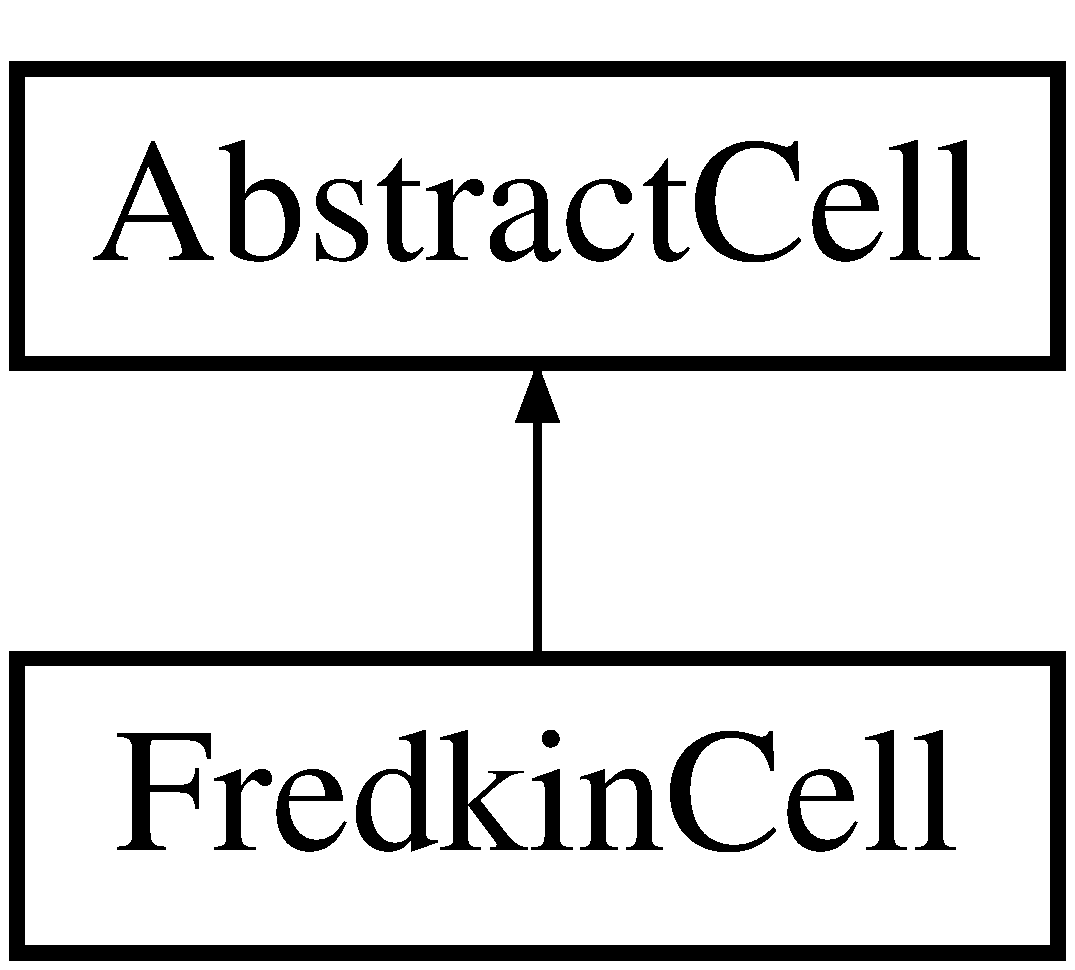
\includegraphics[height=2.000000cm]{classFredkinCell}
\end{center}
\end{figure}
\subsection*{Public Member Functions}
\begin{DoxyCompactItemize}
\item 
\hyperlink{classFredkinCell_ac5bd5726da496a3b3363d9c1b57dccc2}{Fredkin\-Cell} ()
\item 
\hyperlink{classFredkinCell_ada8085f136a647986a3632548d3265e2}{Fredkin\-Cell} (\hyperlink{classAbstractCell}{Abstract\-Cell} $\ast$)
\item 
\hyperlink{classFredkinCell_acc74f231934d691ec6db3346fe1b2c3e}{Fredkin\-Cell} (bool, char)
\item 
\hyperlink{classFredkinCell}{Fredkin\-Cell} $\ast$ \hyperlink{classFredkinCell_a05d7cd1308b23d514e207317fdf06235}{clone} () const 
\item 
void \hyperlink{classFredkinCell_a50b4c7fd707a474c8ddeaefc09818a04}{evolve} (int, \hyperlink{classLife}{Life}$<$ \hyperlink{classFredkinCell}{Fredkin\-Cell} $>$ \&)
\item 
void \hyperlink{classFredkinCell_a662b6ad6a17cda14b4563a17c6ae4eed}{evolve} (int, \hyperlink{classLife}{Life}$<$ \hyperlink{classCell}{Cell} $>$ \&)
\end{DoxyCompactItemize}
\subsection*{Friends}
\begin{DoxyCompactItemize}
\item 
std\-::ostream \& \hyperlink{classFredkinCell_a360e2938139d0e8a1f080b9f8b26a5b8}{operator$<$$<$} (std\-::ostream \&os, const \hyperlink{classFredkinCell}{Fredkin\-Cell} \&fc)
\end{DoxyCompactItemize}
\subsection*{Additional Inherited Members}


\subsection{Constructor \& Destructor Documentation}
\hypertarget{classFredkinCell_ac5bd5726da496a3b3363d9c1b57dccc2}{\index{Fredkin\-Cell@{Fredkin\-Cell}!Fredkin\-Cell@{Fredkin\-Cell}}
\index{Fredkin\-Cell@{Fredkin\-Cell}!FredkinCell@{Fredkin\-Cell}}
\subsubsection[{Fredkin\-Cell}]{\setlength{\rightskip}{0pt plus 5cm}Fredkin\-Cell\-::\-Fredkin\-Cell (
\begin{DoxyParamCaption}
{}
\end{DoxyParamCaption}
)}}\label{classFredkinCell_ac5bd5726da496a3b3363d9c1b57dccc2}
\hypertarget{classFredkinCell_ada8085f136a647986a3632548d3265e2}{\index{Fredkin\-Cell@{Fredkin\-Cell}!Fredkin\-Cell@{Fredkin\-Cell}}
\index{Fredkin\-Cell@{Fredkin\-Cell}!FredkinCell@{Fredkin\-Cell}}
\subsubsection[{Fredkin\-Cell}]{\setlength{\rightskip}{0pt plus 5cm}Fredkin\-Cell\-::\-Fredkin\-Cell (
\begin{DoxyParamCaption}
\item[{{\bf Abstract\-Cell} $\ast$}]{}
\end{DoxyParamCaption}
)}}\label{classFredkinCell_ada8085f136a647986a3632548d3265e2}
\hypertarget{classFredkinCell_acc74f231934d691ec6db3346fe1b2c3e}{\index{Fredkin\-Cell@{Fredkin\-Cell}!Fredkin\-Cell@{Fredkin\-Cell}}
\index{Fredkin\-Cell@{Fredkin\-Cell}!FredkinCell@{Fredkin\-Cell}}
\subsubsection[{Fredkin\-Cell}]{\setlength{\rightskip}{0pt plus 5cm}Fredkin\-Cell\-::\-Fredkin\-Cell (
\begin{DoxyParamCaption}
\item[{bool}]{initial\-\_\-state, }
\item[{char}]{s}
\end{DoxyParamCaption}
)}}\label{classFredkinCell_acc74f231934d691ec6db3346fe1b2c3e}


\subsection{Member Function Documentation}
\hypertarget{classFredkinCell_a05d7cd1308b23d514e207317fdf06235}{\index{Fredkin\-Cell@{Fredkin\-Cell}!clone@{clone}}
\index{clone@{clone}!FredkinCell@{Fredkin\-Cell}}
\subsubsection[{clone}]{\setlength{\rightskip}{0pt plus 5cm}{\bf Fredkin\-Cell} $\ast$ Fredkin\-Cell\-::clone (
\begin{DoxyParamCaption}
{}
\end{DoxyParamCaption}
) const\hspace{0.3cm}{\ttfamily [virtual]}}}\label{classFredkinCell_a05d7cd1308b23d514e207317fdf06235}


Implements \hyperlink{classAbstractCell_a1a95a7ea92b3503e2f042170b6320354}{Abstract\-Cell}.

\hypertarget{classFredkinCell_a50b4c7fd707a474c8ddeaefc09818a04}{\index{Fredkin\-Cell@{Fredkin\-Cell}!evolve@{evolve}}
\index{evolve@{evolve}!FredkinCell@{Fredkin\-Cell}}
\subsubsection[{evolve}]{\setlength{\rightskip}{0pt plus 5cm}void Fredkin\-Cell\-::evolve (
\begin{DoxyParamCaption}
\item[{int}]{index, }
\item[{{\bf Life}$<$ {\bf Fredkin\-Cell} $>$ \&}]{l}
\end{DoxyParamCaption}
)}}\label{classFredkinCell_a50b4c7fd707a474c8ddeaefc09818a04}
\hypertarget{classFredkinCell_a662b6ad6a17cda14b4563a17c6ae4eed}{\index{Fredkin\-Cell@{Fredkin\-Cell}!evolve@{evolve}}
\index{evolve@{evolve}!FredkinCell@{Fredkin\-Cell}}
\subsubsection[{evolve}]{\setlength{\rightskip}{0pt plus 5cm}void Fredkin\-Cell\-::evolve (
\begin{DoxyParamCaption}
\item[{int}]{index, }
\item[{{\bf Life}$<$ {\bf Cell} $>$ \&}]{l}
\end{DoxyParamCaption}
)\hspace{0.3cm}{\ttfamily [virtual]}}}\label{classFredkinCell_a662b6ad6a17cda14b4563a17c6ae4eed}


Implements \hyperlink{classAbstractCell_a3400569dbc73b019698bead4aca5b186}{Abstract\-Cell}.



\subsection{Friends And Related Function Documentation}
\hypertarget{classFredkinCell_a360e2938139d0e8a1f080b9f8b26a5b8}{\index{Fredkin\-Cell@{Fredkin\-Cell}!operator$<$$<$@{operator$<$$<$}}
\index{operator$<$$<$@{operator$<$$<$}!FredkinCell@{Fredkin\-Cell}}
\subsubsection[{operator$<$$<$}]{\setlength{\rightskip}{0pt plus 5cm}std\-::ostream\& operator$<$$<$ (
\begin{DoxyParamCaption}
\item[{std\-::ostream \&}]{os, }
\item[{const {\bf Fredkin\-Cell} \&}]{fc}
\end{DoxyParamCaption}
)\hspace{0.3cm}{\ttfamily [friend]}}}\label{classFredkinCell_a360e2938139d0e8a1f080b9f8b26a5b8}


The documentation for this class was generated from the following files\-:\begin{DoxyCompactItemize}
\item 
\hyperlink{Life_8h}{Life.\-h}\item 
\hyperlink{Life_8c_09_09}{Life.\-c++}\end{DoxyCompactItemize}

\hypertarget{classL__Iterator}{\section{L\-\_\-\-Iterator$<$ T $>$ Class Template Reference}
\label{classL__Iterator}\index{L\-\_\-\-Iterator$<$ T $>$@{L\-\_\-\-Iterator$<$ T $>$}}
}


{\ttfamily \#include $<$Life.\-h$>$}

\subsection*{Public Member Functions}
\begin{DoxyCompactItemize}
\item 
\hyperlink{classL__Iterator_a8e3c67c47cff51cbb1f452768395d0d0}{L\-\_\-\-Iterator} (const T \&v)
\item 
bool \hyperlink{classL__Iterator_a5717579a4a7fc28ca13171f30ca21b2c}{operator==} (const \hyperlink{classL__Iterator}{L\-\_\-\-Iterator}$<$ T $>$ \&rhs) const 
\item 
bool \hyperlink{classL__Iterator_aa7882f06e6e5e446cf9c58e09a8c3384}{operator!=} (const \hyperlink{classL__Iterator}{L\-\_\-\-Iterator}$<$ T $>$ \&rhs) const 
\item 
const T \& \hyperlink{classL__Iterator_a14f900a1b0cfdd3e80d56b7162e9ff08}{operator$\ast$} () const 
\item 
\hyperlink{classL__Iterator}{L\-\_\-\-Iterator}$<$ T $>$ \hyperlink{classL__Iterator_a4eda0697dd0a55dd33ec57b162e9fc95}{operator++} ()
\item 
\hyperlink{classL__Iterator}{L\-\_\-\-Iterator}$<$ T $>$ \hyperlink{classL__Iterator_af5edd5d0fbbb4f096529c21458255e6b}{operator++} (int)
\end{DoxyCompactItemize}
\subsection*{Private Attributes}
\begin{DoxyCompactItemize}
\item 
T \hyperlink{classL__Iterator_a89ecaa2678876d21a2d7be363728340d}{\-\_\-v}
\end{DoxyCompactItemize}


\subsection{Constructor \& Destructor Documentation}
\hypertarget{classL__Iterator_a8e3c67c47cff51cbb1f452768395d0d0}{\index{L\-\_\-\-Iterator@{L\-\_\-\-Iterator}!L\-\_\-\-Iterator@{L\-\_\-\-Iterator}}
\index{L\-\_\-\-Iterator@{L\-\_\-\-Iterator}!L_Iterator@{L\-\_\-\-Iterator}}
\subsubsection[{L\-\_\-\-Iterator}]{\setlength{\rightskip}{0pt plus 5cm}template$<$typename T$>$ {\bf L\-\_\-\-Iterator}$<$ T $>$\-::{\bf L\-\_\-\-Iterator} (
\begin{DoxyParamCaption}
\item[{const T \&}]{v}
\end{DoxyParamCaption}
)\hspace{0.3cm}{\ttfamily [inline]}}}\label{classL__Iterator_a8e3c67c47cff51cbb1f452768395d0d0}


\subsection{Member Function Documentation}
\hypertarget{classL__Iterator_aa7882f06e6e5e446cf9c58e09a8c3384}{\index{L\-\_\-\-Iterator@{L\-\_\-\-Iterator}!operator!=@{operator!=}}
\index{operator!=@{operator!=}!L_Iterator@{L\-\_\-\-Iterator}}
\subsubsection[{operator!=}]{\setlength{\rightskip}{0pt plus 5cm}template$<$typename T$>$ bool {\bf L\-\_\-\-Iterator}$<$ T $>$\-::operator!= (
\begin{DoxyParamCaption}
\item[{const {\bf L\-\_\-\-Iterator}$<$ T $>$ \&}]{rhs}
\end{DoxyParamCaption}
) const\hspace{0.3cm}{\ttfamily [inline]}}}\label{classL__Iterator_aa7882f06e6e5e446cf9c58e09a8c3384}
\hypertarget{classL__Iterator_a14f900a1b0cfdd3e80d56b7162e9ff08}{\index{L\-\_\-\-Iterator@{L\-\_\-\-Iterator}!operator$\ast$@{operator$\ast$}}
\index{operator$\ast$@{operator$\ast$}!L_Iterator@{L\-\_\-\-Iterator}}
\subsubsection[{operator$\ast$}]{\setlength{\rightskip}{0pt plus 5cm}template$<$typename T$>$ const T\& {\bf L\-\_\-\-Iterator}$<$ T $>$\-::operator$\ast$ (
\begin{DoxyParamCaption}
{}
\end{DoxyParamCaption}
) const\hspace{0.3cm}{\ttfamily [inline]}}}\label{classL__Iterator_a14f900a1b0cfdd3e80d56b7162e9ff08}
\hypertarget{classL__Iterator_a4eda0697dd0a55dd33ec57b162e9fc95}{\index{L\-\_\-\-Iterator@{L\-\_\-\-Iterator}!operator++@{operator++}}
\index{operator++@{operator++}!L_Iterator@{L\-\_\-\-Iterator}}
\subsubsection[{operator++}]{\setlength{\rightskip}{0pt plus 5cm}template$<$typename T$>$ {\bf L\-\_\-\-Iterator}$<$T$>$ {\bf L\-\_\-\-Iterator}$<$ T $>$\-::operator++ (
\begin{DoxyParamCaption}
{}
\end{DoxyParamCaption}
)\hspace{0.3cm}{\ttfamily [inline]}}}\label{classL__Iterator_a4eda0697dd0a55dd33ec57b162e9fc95}
\hypertarget{classL__Iterator_af5edd5d0fbbb4f096529c21458255e6b}{\index{L\-\_\-\-Iterator@{L\-\_\-\-Iterator}!operator++@{operator++}}
\index{operator++@{operator++}!L_Iterator@{L\-\_\-\-Iterator}}
\subsubsection[{operator++}]{\setlength{\rightskip}{0pt plus 5cm}template$<$typename T$>$ {\bf L\-\_\-\-Iterator}$<$T$>$ {\bf L\-\_\-\-Iterator}$<$ T $>$\-::operator++ (
\begin{DoxyParamCaption}
\item[{int}]{}
\end{DoxyParamCaption}
)\hspace{0.3cm}{\ttfamily [inline]}}}\label{classL__Iterator_af5edd5d0fbbb4f096529c21458255e6b}
\hypertarget{classL__Iterator_a5717579a4a7fc28ca13171f30ca21b2c}{\index{L\-\_\-\-Iterator@{L\-\_\-\-Iterator}!operator==@{operator==}}
\index{operator==@{operator==}!L_Iterator@{L\-\_\-\-Iterator}}
\subsubsection[{operator==}]{\setlength{\rightskip}{0pt plus 5cm}template$<$typename T$>$ bool {\bf L\-\_\-\-Iterator}$<$ T $>$\-::operator== (
\begin{DoxyParamCaption}
\item[{const {\bf L\-\_\-\-Iterator}$<$ T $>$ \&}]{rhs}
\end{DoxyParamCaption}
) const\hspace{0.3cm}{\ttfamily [inline]}}}\label{classL__Iterator_a5717579a4a7fc28ca13171f30ca21b2c}


\subsection{Member Data Documentation}
\hypertarget{classL__Iterator_a89ecaa2678876d21a2d7be363728340d}{\index{L\-\_\-\-Iterator@{L\-\_\-\-Iterator}!\-\_\-v@{\-\_\-v}}
\index{\-\_\-v@{\-\_\-v}!L_Iterator@{L\-\_\-\-Iterator}}
\subsubsection[{\-\_\-v}]{\setlength{\rightskip}{0pt plus 5cm}template$<$typename T$>$ T {\bf L\-\_\-\-Iterator}$<$ T $>$\-::\-\_\-v\hspace{0.3cm}{\ttfamily [private]}}}\label{classL__Iterator_a89ecaa2678876d21a2d7be363728340d}


The documentation for this class was generated from the following file\-:\begin{DoxyCompactItemize}
\item 
\hyperlink{Life_8h}{Life.\-h}\end{DoxyCompactItemize}

\hypertarget{classLife}{\section{Life$<$ T $>$ Class Template Reference}
\label{classLife}\index{Life$<$ T $>$@{Life$<$ T $>$}}
}


{\ttfamily \#include $<$Life.\-h$>$}

\subsection*{Public Member Functions}
\begin{DoxyCompactItemize}
\item 
\hyperlink{classLife_af49136b65408d89747b5b8157b899aa9}{Life} ()
\item 
\hyperlink{classLife_a38a1876a2663d931054ceb8ec381c951}{Life} (int r, int c, std\-::vector$<$ char $>$ g)
\item 
void \hyperlink{classLife_a7dbf17957d95e5de7eae8b2238926531}{run\-Life} ()
\item 
bool \hyperlink{classLife_a4e4342f7c4a22b0bf34f870f5ac10b44}{inspect\-Neighbors} (int i, char symbol)
\item 
\hyperlink{classL__Iterator}{L\-\_\-\-Iterator}$<$ int $>$ \hyperlink{classLife_a6054856906eebe84367ae17369bc534c}{begin} ()
\item 
\hyperlink{classL__Iterator}{L\-\_\-\-Iterator}$<$ int $>$ \hyperlink{classLife_a13070724cceb1a2d7ab73d2738386c78}{end} ()
\item 
T \hyperlink{classLife_aef6990159e25fb486ea770cc8b47a891}{at} (int index) const 
\end{DoxyCompactItemize}
\subsection*{Private Attributes}
\begin{DoxyCompactItemize}
\item 
int \hyperlink{classLife_ac8b1792a10629f1bfd890ac3acb37510}{rows}
\item 
int \hyperlink{classLife_a65d1a622f32424e9c0a10c7cc051ea58}{columns}
\item 
int \hyperlink{classLife_a53df763a5b9eae675fd8e4d3045bf1ad}{size}
\item 
int \hyperlink{classLife_ad0c82e4ef83bc0b56faf58f28e63e1e2}{population}
\item 
std\-::vector$<$ T $>$ \hyperlink{classLife_a7ecaf21e43796adda4c080cbb33b5198}{grid}
\end{DoxyCompactItemize}
\subsection*{Friends}
\begin{DoxyCompactItemize}
\item 
std\-::ostream \& \hyperlink{classLife_a788d44c7f0bbc3af5090d3e7ccb94c4d}{operator$<$$<$} (std\-::ostream \&os, const \hyperlink{classLife}{Life}$<$ T $>$ \&l)
\end{DoxyCompactItemize}


\subsection{Constructor \& Destructor Documentation}
\hypertarget{classLife_af49136b65408d89747b5b8157b899aa9}{\index{Life@{Life}!Life@{Life}}
\index{Life@{Life}!Life@{Life}}
\subsubsection[{Life}]{\setlength{\rightskip}{0pt plus 5cm}template$<$typename T $>$ {\bf Life}$<$ T $>$\-::{\bf Life} (
\begin{DoxyParamCaption}
{}
\end{DoxyParamCaption}
)\hspace{0.3cm}{\ttfamily [inline]}}}\label{classLife_af49136b65408d89747b5b8157b899aa9}
\hypertarget{classLife_a38a1876a2663d931054ceb8ec381c951}{\index{Life@{Life}!Life@{Life}}
\index{Life@{Life}!Life@{Life}}
\subsubsection[{Life}]{\setlength{\rightskip}{0pt plus 5cm}template$<$typename T $>$ {\bf Life}$<$ T $>$\-::{\bf Life} (
\begin{DoxyParamCaption}
\item[{int}]{r, }
\item[{int}]{c, }
\item[{std\-::vector$<$ char $>$}]{g}
\end{DoxyParamCaption}
)\hspace{0.3cm}{\ttfamily [inline]}}}\label{classLife_a38a1876a2663d931054ceb8ec381c951}


\subsection{Member Function Documentation}
\hypertarget{classLife_aef6990159e25fb486ea770cc8b47a891}{\index{Life@{Life}!at@{at}}
\index{at@{at}!Life@{Life}}
\subsubsection[{at}]{\setlength{\rightskip}{0pt plus 5cm}template$<$typename T $>$ T {\bf Life}$<$ T $>$\-::at (
\begin{DoxyParamCaption}
\item[{int}]{index}
\end{DoxyParamCaption}
) const\hspace{0.3cm}{\ttfamily [inline]}}}\label{classLife_aef6990159e25fb486ea770cc8b47a891}
\hypertarget{classLife_a6054856906eebe84367ae17369bc534c}{\index{Life@{Life}!begin@{begin}}
\index{begin@{begin}!Life@{Life}}
\subsubsection[{begin}]{\setlength{\rightskip}{0pt plus 5cm}template$<$typename T $>$ {\bf L\-\_\-\-Iterator}$<$int$>$ {\bf Life}$<$ T $>$\-::begin (
\begin{DoxyParamCaption}
{}
\end{DoxyParamCaption}
)\hspace{0.3cm}{\ttfamily [inline]}}}\label{classLife_a6054856906eebe84367ae17369bc534c}
\hypertarget{classLife_a13070724cceb1a2d7ab73d2738386c78}{\index{Life@{Life}!end@{end}}
\index{end@{end}!Life@{Life}}
\subsubsection[{end}]{\setlength{\rightskip}{0pt plus 5cm}template$<$typename T $>$ {\bf L\-\_\-\-Iterator}$<$int$>$ {\bf Life}$<$ T $>$\-::end (
\begin{DoxyParamCaption}
{}
\end{DoxyParamCaption}
)\hspace{0.3cm}{\ttfamily [inline]}}}\label{classLife_a13070724cceb1a2d7ab73d2738386c78}
\hypertarget{classLife_a4e4342f7c4a22b0bf34f870f5ac10b44}{\index{Life@{Life}!inspect\-Neighbors@{inspect\-Neighbors}}
\index{inspect\-Neighbors@{inspect\-Neighbors}!Life@{Life}}
\subsubsection[{inspect\-Neighbors}]{\setlength{\rightskip}{0pt plus 5cm}template$<$typename T $>$ bool {\bf Life}$<$ T $>$\-::inspect\-Neighbors (
\begin{DoxyParamCaption}
\item[{int}]{i, }
\item[{char}]{symbol}
\end{DoxyParamCaption}
)\hspace{0.3cm}{\ttfamily [inline]}}}\label{classLife_a4e4342f7c4a22b0bf34f870f5ac10b44}
\hypertarget{classLife_a7dbf17957d95e5de7eae8b2238926531}{\index{Life@{Life}!run\-Life@{run\-Life}}
\index{run\-Life@{run\-Life}!Life@{Life}}
\subsubsection[{run\-Life}]{\setlength{\rightskip}{0pt plus 5cm}template$<$typename T $>$ void {\bf Life}$<$ T $>$\-::run\-Life (
\begin{DoxyParamCaption}
{}
\end{DoxyParamCaption}
)\hspace{0.3cm}{\ttfamily [inline]}}}\label{classLife_a7dbf17957d95e5de7eae8b2238926531}


\subsection{Friends And Related Function Documentation}
\hypertarget{classLife_a788d44c7f0bbc3af5090d3e7ccb94c4d}{\index{Life@{Life}!operator$<$$<$@{operator$<$$<$}}
\index{operator$<$$<$@{operator$<$$<$}!Life@{Life}}
\subsubsection[{operator$<$$<$}]{\setlength{\rightskip}{0pt plus 5cm}template$<$typename T $>$ std\-::ostream\& operator$<$$<$ (
\begin{DoxyParamCaption}
\item[{std\-::ostream \&}]{os, }
\item[{const {\bf Life}$<$ T $>$ \&}]{l}
\end{DoxyParamCaption}
)\hspace{0.3cm}{\ttfamily [friend]}}}\label{classLife_a788d44c7f0bbc3af5090d3e7ccb94c4d}


\subsection{Member Data Documentation}
\hypertarget{classLife_a65d1a622f32424e9c0a10c7cc051ea58}{\index{Life@{Life}!columns@{columns}}
\index{columns@{columns}!Life@{Life}}
\subsubsection[{columns}]{\setlength{\rightskip}{0pt plus 5cm}template$<$typename T $>$ int {\bf Life}$<$ T $>$\-::columns\hspace{0.3cm}{\ttfamily [private]}}}\label{classLife_a65d1a622f32424e9c0a10c7cc051ea58}
\hypertarget{classLife_a7ecaf21e43796adda4c080cbb33b5198}{\index{Life@{Life}!grid@{grid}}
\index{grid@{grid}!Life@{Life}}
\subsubsection[{grid}]{\setlength{\rightskip}{0pt plus 5cm}template$<$typename T $>$ std\-::vector$<$T$>$ {\bf Life}$<$ T $>$\-::grid\hspace{0.3cm}{\ttfamily [private]}}}\label{classLife_a7ecaf21e43796adda4c080cbb33b5198}
\hypertarget{classLife_ad0c82e4ef83bc0b56faf58f28e63e1e2}{\index{Life@{Life}!population@{population}}
\index{population@{population}!Life@{Life}}
\subsubsection[{population}]{\setlength{\rightskip}{0pt plus 5cm}template$<$typename T $>$ int {\bf Life}$<$ T $>$\-::population\hspace{0.3cm}{\ttfamily [private]}}}\label{classLife_ad0c82e4ef83bc0b56faf58f28e63e1e2}
\hypertarget{classLife_ac8b1792a10629f1bfd890ac3acb37510}{\index{Life@{Life}!rows@{rows}}
\index{rows@{rows}!Life@{Life}}
\subsubsection[{rows}]{\setlength{\rightskip}{0pt plus 5cm}template$<$typename T $>$ int {\bf Life}$<$ T $>$\-::rows\hspace{0.3cm}{\ttfamily [private]}}}\label{classLife_ac8b1792a10629f1bfd890ac3acb37510}
\hypertarget{classLife_a53df763a5b9eae675fd8e4d3045bf1ad}{\index{Life@{Life}!size@{size}}
\index{size@{size}!Life@{Life}}
\subsubsection[{size}]{\setlength{\rightskip}{0pt plus 5cm}template$<$typename T $>$ int {\bf Life}$<$ T $>$\-::size\hspace{0.3cm}{\ttfamily [private]}}}\label{classLife_a53df763a5b9eae675fd8e4d3045bf1ad}


The documentation for this class was generated from the following file\-:\begin{DoxyCompactItemize}
\item 
\hyperlink{Life_8h}{Life.\-h}\end{DoxyCompactItemize}

\chapter{File Documentation}
\hypertarget{Life_8c_09_09}{\section{Life.\-c++ File Reference}
\label{Life_8c_09_09}\index{Life.\-c++@{Life.\-c++}}
}
{\ttfamily \#include $<$iostream$>$}\\*
{\ttfamily \#include $<$string$>$}\\*
{\ttfamily \#include $<$sstream$>$}\\*
{\ttfamily \#include $<$vector$>$}\\*
{\ttfamily \#include $<$cstring$>$}\\*
{\ttfamily \#include \char`\"{}Life.\-h\char`\"{}}\\*
\subsection*{Functions}
\begin{DoxyCompactItemize}
\item 
ostream \& \hyperlink{Life_8c_09_09_ae254f299bfa3722186f36aaee153f869}{operator$<$$<$} (ostream \&os, const \hyperlink{classCell}{Cell} \&c)
\item 
ostream \& \hyperlink{Life_8c_09_09_a6ce5e46e5ef2f35223787462a562d066}{operator$<$$<$} (ostream \&os, const \hyperlink{classConwayCell}{Conway\-Cell} \&cc)
\item 
ostream \& \hyperlink{Life_8c_09_09_af9362bce0b651c9fce1dd255e55290d8}{operator$<$$<$} (ostream \&os, const \hyperlink{classFredkinCell}{Fredkin\-Cell} \&fc)
\item 
void \hyperlink{Life_8c_09_09_a1a58f997987d528f1659dcbb7406c7b5}{enact\-\_\-life} (istream \&r, ostream \&w)
\end{DoxyCompactItemize}


\subsection{Function Documentation}
\hypertarget{Life_8c_09_09_a1a58f997987d528f1659dcbb7406c7b5}{\index{Life.\-c++@{Life.\-c++}!enact\-\_\-life@{enact\-\_\-life}}
\index{enact\-\_\-life@{enact\-\_\-life}!Life.c++@{Life.\-c++}}
\subsubsection[{enact\-\_\-life}]{\setlength{\rightskip}{0pt plus 5cm}void enact\-\_\-life (
\begin{DoxyParamCaption}
\item[{istream \&}]{r, }
\item[{ostream \&}]{w}
\end{DoxyParamCaption}
)}}\label{Life_8c_09_09_a1a58f997987d528f1659dcbb7406c7b5}
\hypertarget{Life_8c_09_09_ae254f299bfa3722186f36aaee153f869}{\index{Life.\-c++@{Life.\-c++}!operator$<$$<$@{operator$<$$<$}}
\index{operator$<$$<$@{operator$<$$<$}!Life.c++@{Life.\-c++}}
\subsubsection[{operator$<$$<$}]{\setlength{\rightskip}{0pt plus 5cm}ostream\& operator$<$$<$ (
\begin{DoxyParamCaption}
\item[{ostream \&}]{os, }
\item[{const {\bf Cell} \&}]{c}
\end{DoxyParamCaption}
)}}\label{Life_8c_09_09_ae254f299bfa3722186f36aaee153f869}
\hypertarget{Life_8c_09_09_a6ce5e46e5ef2f35223787462a562d066}{\index{Life.\-c++@{Life.\-c++}!operator$<$$<$@{operator$<$$<$}}
\index{operator$<$$<$@{operator$<$$<$}!Life.c++@{Life.\-c++}}
\subsubsection[{operator$<$$<$}]{\setlength{\rightskip}{0pt plus 5cm}ostream\& operator$<$$<$ (
\begin{DoxyParamCaption}
\item[{ostream \&}]{os, }
\item[{const {\bf Conway\-Cell} \&}]{cc}
\end{DoxyParamCaption}
)}}\label{Life_8c_09_09_a6ce5e46e5ef2f35223787462a562d066}
\hypertarget{Life_8c_09_09_af9362bce0b651c9fce1dd255e55290d8}{\index{Life.\-c++@{Life.\-c++}!operator$<$$<$@{operator$<$$<$}}
\index{operator$<$$<$@{operator$<$$<$}!Life.c++@{Life.\-c++}}
\subsubsection[{operator$<$$<$}]{\setlength{\rightskip}{0pt plus 5cm}ostream\& operator$<$$<$ (
\begin{DoxyParamCaption}
\item[{ostream \&}]{os, }
\item[{const {\bf Fredkin\-Cell} \&}]{fc}
\end{DoxyParamCaption}
)}}\label{Life_8c_09_09_af9362bce0b651c9fce1dd255e55290d8}

\hypertarget{Life_8h}{\section{Life.\-h File Reference}
\label{Life_8h}\index{Life.\-h@{Life.\-h}}
}
{\ttfamily \#include $<$iostream$>$}\\*
{\ttfamily \#include $<$vector$>$}\\*
{\ttfamily \#include $<$iterator$>$}\\*
{\ttfamily \#include $<$type\-\_\-traits$>$}\\*
\subsection*{Classes}
\begin{DoxyCompactItemize}
\item 
class \hyperlink{classLife}{Life$<$ T $>$}
\item 
class \hyperlink{classAbstractCell}{Abstract\-Cell}
\item 
class \hyperlink{classConwayCell}{Conway\-Cell}
\item 
class \hyperlink{classFredkinCell}{Fredkin\-Cell}
\item 
class \hyperlink{classCell}{Cell}
\item 
class \hyperlink{classL__Iterator}{L\-\_\-\-Iterator$<$ T $>$}
\item 
class \hyperlink{classLife}{Life$<$ T $>$}
\end{DoxyCompactItemize}
\subsection*{Functions}
\begin{DoxyCompactItemize}
\item 
void \hyperlink{Life_8h_af54e2f2dc7bf238025c8b2886f66da62}{enact\-\_\-life} (std\-::istream \&r, std\-::ostream \&w)
\end{DoxyCompactItemize}


\subsection{Function Documentation}
\hypertarget{Life_8h_af54e2f2dc7bf238025c8b2886f66da62}{\index{Life.\-h@{Life.\-h}!enact\-\_\-life@{enact\-\_\-life}}
\index{enact\-\_\-life@{enact\-\_\-life}!Life.h@{Life.\-h}}
\subsubsection[{enact\-\_\-life}]{\setlength{\rightskip}{0pt plus 5cm}void enact\-\_\-life (
\begin{DoxyParamCaption}
\item[{std\-::istream \&}]{r, }
\item[{std\-::ostream \&}]{w}
\end{DoxyParamCaption}
)}}\label{Life_8h_af54e2f2dc7bf238025c8b2886f66da62}

\hypertarget{LifeTestMaker_8c_09_09}{\section{Life\-Test\-Maker.\-c++ File Reference}
\label{LifeTestMaker_8c_09_09}\index{Life\-Test\-Maker.\-c++@{Life\-Test\-Maker.\-c++}}
}
{\ttfamily \#include $<$iostream$>$}\\*
{\ttfamily \#include $<$vector$>$}\\*
{\ttfamily \#include $<$cstdlib$>$}\\*
\subsection*{Functions}
\begin{DoxyCompactItemize}
\item 
int \hyperlink{LifeTestMaker_8c_09_09_ae66f6b31b5ad750f1fe042a706a4e3d4}{main} ()
\end{DoxyCompactItemize}


\subsection{Function Documentation}
\hypertarget{LifeTestMaker_8c_09_09_ae66f6b31b5ad750f1fe042a706a4e3d4}{\index{Life\-Test\-Maker.\-c++@{Life\-Test\-Maker.\-c++}!main@{main}}
\index{main@{main}!LifeTestMaker.c++@{Life\-Test\-Maker.\-c++}}
\subsubsection[{main}]{\setlength{\rightskip}{0pt plus 5cm}int main (
\begin{DoxyParamCaption}
{}
\end{DoxyParamCaption}
)}}\label{LifeTestMaker_8c_09_09_ae66f6b31b5ad750f1fe042a706a4e3d4}

\hypertarget{README_8md}{\section{R\-E\-A\-D\-M\-E.\-md File Reference}
\label{README_8md}\index{R\-E\-A\-D\-M\-E.\-md@{R\-E\-A\-D\-M\-E.\-md}}
}

\hypertarget{RunLife_8c_09_09}{\section{Run\-Life.\-c++ File Reference}
\label{RunLife_8c_09_09}\index{Run\-Life.\-c++@{Run\-Life.\-c++}}
}
{\ttfamily \#include $<$iostream$>$}\\*
{\ttfamily \#include \char`\"{}Life.\-h\char`\"{}}\\*
\subsection*{Functions}
\begin{DoxyCompactItemize}
\item 
int \hyperlink{RunLife_8c_09_09_ae66f6b31b5ad750f1fe042a706a4e3d4}{main} ()
\end{DoxyCompactItemize}


\subsection{Function Documentation}
\hypertarget{RunLife_8c_09_09_ae66f6b31b5ad750f1fe042a706a4e3d4}{\index{Run\-Life.\-c++@{Run\-Life.\-c++}!main@{main}}
\index{main@{main}!RunLife.c++@{Run\-Life.\-c++}}
\subsubsection[{main}]{\setlength{\rightskip}{0pt plus 5cm}int main (
\begin{DoxyParamCaption}
{}
\end{DoxyParamCaption}
)}}\label{RunLife_8c_09_09_ae66f6b31b5ad750f1fe042a706a4e3d4}

\hypertarget{TestLife_8c_09_09}{\section{Test\-Life.\-c++ File Reference}
\label{TestLife_8c_09_09}\index{Test\-Life.\-c++@{Test\-Life.\-c++}}
}
{\ttfamily \#include $<$iostream$>$}\\*
{\ttfamily \#include $<$sstream$>$}\\*
{\ttfamily \#include $<$string$>$}\\*
{\ttfamily \#include \char`\"{}Life.\-h\char`\"{}}\\*
{\ttfamily \#include \char`\"{}gtest/gtest.\-h\char`\"{}}\\*
\subsection*{Functions}
\begin{DoxyCompactItemize}
\item 
\hyperlink{TestLife_8c_09_09_ab5a44d50c75c216949c67ebdc337020a}{T\-E\-S\-T} (Abstract\-Cell\-Fixture, abstract\-\_\-cell\-\_\-can\-Mutate\-\_\-1)
\item 
\hyperlink{TestLife_8c_09_09_a966b2cb59e53ae074d48f1ecc72ee0d9}{T\-E\-S\-T} (Abstract\-Cell\-Fixture, abstract\-\_\-cell\-\_\-can\-Mutate\-\_\-2)
\item 
\hyperlink{TestLife_8c_09_09_a968aec6ca187d1bee8488988c92c6458}{T\-E\-S\-T} (Abstract\-Cell\-Fixture, abstract\-\_\-cell\-\_\-can\-Mutate\-\_\-3)
\item 
\hyperlink{TestLife_8c_09_09_a4778ce2d8eedc94f57d606df25b8925c}{T\-E\-S\-T} (Abstract\-Cell\-Fixture, abstract\-\_\-cell\-\_\-change\-State\-\_\-1)
\item 
\hyperlink{TestLife_8c_09_09_a65c4a9eac62b7f18124415429fd46149}{T\-E\-S\-T} (Abstract\-Cell\-Fixture, abstract\-\_\-cell\-\_\-change\-State\-\_\-2)
\item 
\hyperlink{TestLife_8c_09_09_a942687f4d40953798ee276d728b4fafc}{T\-E\-S\-T} (Abstract\-Cell\-Fixture, abstract\-\_\-cell\-\_\-change\-State\-\_\-3)
\item 
\hyperlink{TestLife_8c_09_09_a4059eb29bfc3a4d73328c13750a61fc5}{T\-E\-S\-T} (Abstract\-Cell\-Fixture, abstract\-\_\-cell\-\_\-is\-Alive\-\_\-1)
\item 
\hyperlink{TestLife_8c_09_09_a6ad979593e6b116542dda687f8f42e12}{T\-E\-S\-T} (Abstract\-Cell\-Fixture, abstract\-\_\-cell\-\_\-is\-Alive\-\_\-2)
\item 
\hyperlink{TestLife_8c_09_09_a003eec48faf2d762aaac4e5d59cee0a4}{T\-E\-S\-T} (Abstract\-Cell\-Fixture, abstract\-\_\-cell\-\_\-is\-Alive\-\_\-3)
\item 
\hyperlink{TestLife_8c_09_09_ae05a09392d273da0ad2e5dd1b4f390c8}{T\-E\-S\-T} (Conway\-Cell\-Fixture, conway\-\_\-cell\-\_\-default\-\_\-constructor\-\_\-1)
\item 
\hyperlink{TestLife_8c_09_09_af325567419308e8272dd009bc6681351}{T\-E\-S\-T} (Conway\-Cell\-Fixture, conway\-\_\-cell\-\_\-default\-\_\-constructor\-\_\-2)
\item 
\hyperlink{TestLife_8c_09_09_ad54811c8d0ace242c232ade1c8d03ddc}{T\-E\-S\-T} (Conway\-Cell\-Fixture, conway\-\_\-cell\-\_\-default\-\_\-constructor\-\_\-3)
\item 
\hyperlink{TestLife_8c_09_09_ab66e7ee0054b4aca74d5f96132449172}{T\-E\-S\-T} (Conway\-Cell\-Fixture, conway\-\_\-cell\-\_\-custom\-\_\-constructor\-\_\-1)
\item 
\hyperlink{TestLife_8c_09_09_aee413901b77be61d37a3813e21b33652}{T\-E\-S\-T} (Conway\-Cell\-Fixture, conway\-\_\-cell\-\_\-custom\-\_\-constructor\-\_\-2)
\item 
\hyperlink{TestLife_8c_09_09_ae601dfbb1857b791778af72bd0cc8fce}{T\-E\-S\-T} (Conway\-Cell\-Fixture, conway\-\_\-cell\-\_\-custom\-\_\-constructor\-\_\-3)
\item 
\hyperlink{TestLife_8c_09_09_a68d33f17a57c52636d86f501a47eac1f}{T\-E\-S\-T} (Conway\-Cell\-Fixture, conway\-\_\-cell\-\_\-clone\-\_\-1)
\item 
\hyperlink{TestLife_8c_09_09_adcef80dd8b5f5c0ed50db26cdde5b0b6}{T\-E\-S\-T} (Conway\-Cell\-Fixture, conway\-\_\-cell\-\_\-clone\-\_\-2)
\item 
\hyperlink{TestLife_8c_09_09_ae730fcdb1bfe00fa4037eb4133c5ba27}{T\-E\-S\-T} (Conway\-Cell\-Fixture, conway\-\_\-cell\-\_\-clone\-\_\-3)
\item 
\hyperlink{TestLife_8c_09_09_a363ded67c8747ad8eb10046c6a32a840}{T\-E\-S\-T} (Conway\-Cell\-Fixture, conway\-\_\-cell\-\_\-evolve\-\_\-\-Life\-\_\-\-Cell\-\_\-1)
\item 
\hyperlink{TestLife_8c_09_09_a5be40abdf979ee9a370f6b3d1e981c19}{T\-E\-S\-T} (Conway\-Cell\-Fixture, conway\-\_\-cell\-\_\-evolve\-\_\-\-Life\-\_\-\-Cell\-\_\-2)
\item 
\hyperlink{TestLife_8c_09_09_a1892a8639271cab9c6bcd42eed5ca03b}{T\-E\-S\-T} (Conway\-Cell\-Fixture, conway\-\_\-cell\-\_\-evolve\-\_\-\-Life\-\_\-\-Cell\-\_\-3)
\item 
\hyperlink{TestLife_8c_09_09_ac4044984ea6b086b65015c3df19a8595}{T\-E\-S\-T} (Conway\-Cell\-Fixture, conway\-\_\-cell\-\_\-evolve\-\_\-\-Life\-\_\-\-Conway\-Cell\-\_\-1)
\item 
\hyperlink{TestLife_8c_09_09_ac828a2ec42cb6f0c4b4e9088ce611509}{T\-E\-S\-T} (Conway\-Cell\-Fixture, conway\-\_\-cell\-\_\-evolve\-\_\-\-Life\-\_\-\-Conway\-Cell\-\_\-2)
\item 
\hyperlink{TestLife_8c_09_09_a5029723212553c88dfdb43a265d01e30}{T\-E\-S\-T} (Conway\-Cell\-Fixture, conway\-\_\-cell\-\_\-evolve\-\_\-\-Life\-\_\-\-Conway\-Cell\-\_\-3)
\item 
\hyperlink{TestLife_8c_09_09_a11561a58720be29ef22cb6250d8ea5b8}{T\-E\-S\-T} (Fredkin\-Cell\-Fixture, fredkin\-\_\-cell\-\_\-default\-\_\-constructor\-\_\-1)
\item 
\hyperlink{TestLife_8c_09_09_ac07dedf2c2fc954a89a68b35dcb82255}{T\-E\-S\-T} (Fredkin\-Cell\-Fixture, fredkin\-\_\-cell\-\_\-default\-\_\-constructor\-\_\-2)
\item 
\hyperlink{TestLife_8c_09_09_a9ec000791dfb31181017aab9a918877f}{T\-E\-S\-T} (Fredkin\-Cell\-Fixture, fredkin\-\_\-cell\-\_\-default\-\_\-constructor\-\_\-3)
\item 
\hyperlink{TestLife_8c_09_09_a883a069ea5826c88bb0293cf9e7ce932}{T\-E\-S\-T} (Fredkin\-Cell\-Fixture, fredkin\-\_\-cell\-\_\-custom\-\_\-constructor\-\_\-1)
\item 
\hyperlink{TestLife_8c_09_09_a0222a8b2db9232cbf4487b3819e5a12b}{T\-E\-S\-T} (Fredkin\-Cell\-Fixture, fredkin\-\_\-cell\-\_\-custom\-\_\-constructor\-\_\-2)
\item 
\hyperlink{TestLife_8c_09_09_a6ed58a7b97d8453b756cc1e3fa2cc6a2}{T\-E\-S\-T} (Fredkin\-Cell\-Fixture, fredkin\-\_\-cell\-\_\-custom\-\_\-constructor\-\_\-3)
\item 
\hyperlink{TestLife_8c_09_09_ab6fde36e46c2eafb7b82b5e8ae5ae2a9}{T\-E\-S\-T} (Fredkin\-Cell\-Fixture, fredkin\-\_\-cell\-\_\-clone\-\_\-1)
\item 
\hyperlink{TestLife_8c_09_09_ab5940d52fb05c2596d6b2a3b6eb84b83}{T\-E\-S\-T} (Fredkin\-Cell\-Fixture, fredkin\-\_\-cell\-\_\-clone\-\_\-2)
\item 
\hyperlink{TestLife_8c_09_09_a3a0ca36eaa1d7e68f2d70bdc2645e416}{T\-E\-S\-T} (Fredkin\-Cell\-Fixture, fredkin\-\_\-cell\-\_\-clone\-\_\-3)
\item 
\hyperlink{TestLife_8c_09_09_a14f7877b81d8edf8f5a26ceed7f2b7a5}{T\-E\-S\-T} (Fredkin\-Cell\-Fixture, fredkin\-\_\-cell\-\_\-evolve\-\_\-\-Life\-\_\-\-Cell\-\_\-1)
\item 
\hyperlink{TestLife_8c_09_09_a7e6d2bb9937aef89c8c1ab62382f974e}{T\-E\-S\-T} (Fredkin\-Cell\-Fixture, fredkin\-\_\-cell\-\_\-evolve\-\_\-\-Life\-\_\-\-Cell\-\_\-2)
\item 
\hyperlink{TestLife_8c_09_09_a0a8d0abdcc478973226346770ac63119}{T\-E\-S\-T} (Fredkin\-Cell\-Fixture, fredkin\-\_\-cell\-\_\-evolve\-\_\-\-Life\-\_\-\-Cell\-\_\-3)
\item 
\hyperlink{TestLife_8c_09_09_a71fd900d774e6cd68a4169c88a076505}{T\-E\-S\-T} (Fredkin\-Cell\-Fixture, fredkin\-\_\-cell\-\_\-evolve\-\_\-\-Life\-\_\-\-Fredkin\-Cell\-\_\-1)
\item 
\hyperlink{TestLife_8c_09_09_a34f5bbdc64c1eb559bf42d44a6cb0cdb}{T\-E\-S\-T} (Fredkin\-Cell\-Fixture, fredkin\-\_\-cell\-\_\-evolve\-\_\-\-Life\-\_\-\-Fredkin\-Cell\-\_\-2)
\item 
\hyperlink{TestLife_8c_09_09_a7c15bbf7fe27df22b5b1d21665a81994}{T\-E\-S\-T} (Fredkin\-Cell\-Fixture, fredkin\-\_\-cell\-\_\-evolve\-\_\-\-Life\-\_\-\-Fredkin\-Cell\-\_\-3)
\item 
\hyperlink{TestLife_8c_09_09_a07dfb3723ef1406df4bb0900ab5c3491}{T\-E\-S\-T} (Cell\-Fixture, cell\-\_\-default\-\_\-constructor\-\_\-1)
\item 
\hyperlink{TestLife_8c_09_09_addd9019ee5a3d4005ad6d0a72afd0c31}{T\-E\-S\-T} (Cell\-Fixture, cell\-\_\-default\-\_\-constructor\-\_\-2)
\item 
\hyperlink{TestLife_8c_09_09_aa06ceb13f0a8a615783ff69d6e82b629}{T\-E\-S\-T} (Cell\-Fixture, cell\-\_\-default\-\_\-constructor\-\_\-3)
\item 
\hyperlink{TestLife_8c_09_09_a5e251ab89b588434b5935c5b7a63ab20}{T\-E\-S\-T} (Cell\-Fixture, cell\-\_\-abstract\-Cell\-\_\-constructor\-\_\-1)
\item 
\hyperlink{TestLife_8c_09_09_a9e21b7ebd889cf400281d244bd18376b}{T\-E\-S\-T} (Cell\-Fixture, cell\-\_\-abstract\-Cell\-\_\-constructor\-\_\-2)
\item 
\hyperlink{TestLife_8c_09_09_a94ccfd749211d36c7279bb7d1075cd82}{T\-E\-S\-T} (Cell\-Fixture, cell\-\_\-abstract\-Cell\-\_\-constructor\-\_\-3)
\item 
\hyperlink{TestLife_8c_09_09_a67e9026bcd717e19b7ba7a4df9ad400c}{T\-E\-S\-T} (Cell\-Fixture, cell\-\_\-abstract\-Cell\-\_\-constructor\-\_\-4)
\item 
\hyperlink{TestLife_8c_09_09_a704254ff5e55befb3957b57f80f0551e}{T\-E\-S\-T} (Cell\-Fixture, cell\-\_\-abstract\-Cell\-\_\-constructor\-\_\-5)
\item 
\hyperlink{TestLife_8c_09_09_a4b310f8cfe5ce4beb15d40bab4296d8e}{T\-E\-S\-T} (Cell\-Fixture, cell\-\_\-abstract\-Cell\-\_\-constructor\-\_\-6)
\item 
\hyperlink{TestLife_8c_09_09_a8999e664efa1fc6cc3b323b54165f78d}{T\-E\-S\-T} (Cell\-Fixture, cell\-\_\-abstract\-Cell\-\_\-constructor\-\_\-7)
\item 
\hyperlink{TestLife_8c_09_09_ab2b3084f8b8d3c0ce64caeb8109ec505}{T\-E\-S\-T} (Cell\-Fixture, cell\-\_\-abstract\-Cell\-\_\-constructor\-\_\-8)
\item 
\hyperlink{TestLife_8c_09_09_ab2568b1291e1c89a398ffba18f873caa}{T\-E\-S\-T} (Cell\-Fixture, cell\-\_\-custom\-\_\-constructor\-\_\-1)
\item 
\hyperlink{TestLife_8c_09_09_a5e47739504022e04ed73126ebcfd9f6e}{T\-E\-S\-T} (Cell\-Fixture, cell\-\_\-custom\-\_\-constructor\-\_\-2)
\item 
\hyperlink{TestLife_8c_09_09_aeb834b4af9c0919f4c392e9d990f5ee7}{T\-E\-S\-T} (Cell\-Fixture, cell\-\_\-custom\-\_\-constructor\-\_\-3)
\item 
\hyperlink{TestLife_8c_09_09_afad14577d2166ba390c3597445d9c323}{T\-E\-S\-T} (Cell\-Fixture, cell\-\_\-custom\-\_\-constructor\-\_\-4)
\item 
\hyperlink{TestLife_8c_09_09_ab5c3cf0b256379e78a37d26915d8ac12}{T\-E\-S\-T} (Cell\-Fixture, cell\-\_\-assignment\-\_\-operator\-\_\-1)
\item 
\hyperlink{TestLife_8c_09_09_a40752c5e203cb85cd850cca5917e33da}{T\-E\-S\-T} (Cell\-Fixture, cell\-\_\-assignment\-\_\-operator\-\_\-2)
\item 
\hyperlink{TestLife_8c_09_09_a0d94165bddd6dc6db849355ab8d20b14}{T\-E\-S\-T} (Cell\-Fixture, cell\-\_\-assignment\-\_\-operator\-\_\-3)
\item 
\hyperlink{TestLife_8c_09_09_adadc23d489b7b4ddfd26a890ed8a5a41}{T\-E\-S\-T} (Cell\-Fixture, cell\-\_\-assignment\-\_\-operator\-\_\-4)
\item 
\hyperlink{TestLife_8c_09_09_a71e01d5c299761ea54137ec260dd300b}{T\-E\-S\-T} (Cell\-Fixture, cell\-\_\-evolve\-\_\-1)
\item 
\hyperlink{TestLife_8c_09_09_ae73424fa1281ec53f81cb0684bbef79b}{T\-E\-S\-T} (Cell\-Fixture, cell\-\_\-evolve\-\_\-2)
\item 
\hyperlink{TestLife_8c_09_09_a16fdbdfc11b2031b8a42d2b980eed204}{T\-E\-S\-T} (Cell\-Fixture, cell\-\_\-evolve\-\_\-3)
\item 
\hyperlink{TestLife_8c_09_09_a92544f6316786e1fb23f78338afb8823}{T\-E\-S\-T} (Cell\-Fixture, cell\-\_\-can\-Mutate\-\_\-1)
\item 
\hyperlink{TestLife_8c_09_09_ac1ae05c2f1233c068b3db6ddc822dc2c}{T\-E\-S\-T} (Cell\-Fixture, cell\-\_\-can\-Mutate\-\_\-2)
\item 
\hyperlink{TestLife_8c_09_09_a25eefc995c4a0737019fc5a48958e1e7}{T\-E\-S\-T} (Cell\-Fixture, cell\-\_\-can\-Mutate\-\_\-3)
\item 
\hyperlink{TestLife_8c_09_09_ab3e9cb0299c6cc0a061f7ed029cf8bc4}{T\-E\-S\-T} (Cell\-Fixture, cell\-\_\-change\-State\-\_\-1)
\item 
\hyperlink{TestLife_8c_09_09_a9a541e160c9b320c223d651604560bd4}{T\-E\-S\-T} (Cell\-Fixture, cell\-\_\-change\-State\-\_\-2)
\item 
\hyperlink{TestLife_8c_09_09_afca6c2555df9490bb1272abe65a18897}{T\-E\-S\-T} (Cell\-Fixture, cell\-\_\-change\-State\-\_\-3)
\item 
\hyperlink{TestLife_8c_09_09_a6bbe0000d4b7d4e0c06f39ebb706fd12}{T\-E\-S\-T} (Cell\-Fixture, cell\-\_\-change\-State\-\_\-4)
\item 
\hyperlink{TestLife_8c_09_09_adbc36c1e61b8bd661ec4ca18b262b0d6}{T\-E\-S\-T} (Cell\-Fixture, cell\-\_\-is\-Alive\-\_\-1)
\item 
\hyperlink{TestLife_8c_09_09_aba36a37810b4c8ac7a33fe312f037d15}{T\-E\-S\-T} (Cell\-Fixture, cell\-\_\-is\-Alive\-\_\-2)
\item 
\hyperlink{TestLife_8c_09_09_a6819aa700e86d15276187df0133c998a}{T\-E\-S\-T} (Cell\-Fixture, cell\-\_\-is\-Alive\-\_\-3)
\item 
\hyperlink{TestLife_8c_09_09_a2b8000936f49749f0c61e89368116f2c}{T\-E\-S\-T} (Cell\-Fixture, cell\-\_\-is\-Alive\-\_\-4)
\item 
\hyperlink{TestLife_8c_09_09_af295f80b7338e9a9de75522836d51107}{T\-E\-S\-T} (L\-\_\-\-Iterator\-Fixture, constructor\-\_\-1)
\item 
\hyperlink{TestLife_8c_09_09_a29de2eb115746d625d5c86eae3446240}{T\-E\-S\-T} (L\-\_\-\-Iterator\-Fixture, constructor\-\_\-2)
\item 
\hyperlink{TestLife_8c_09_09_a6edd6007d7159bed47a9945e8466a95e}{T\-E\-S\-T} (L\-\_\-\-Iterator\-Fixture, constructor\-\_\-3)
\item 
\hyperlink{TestLife_8c_09_09_af4b17935b8fc460e7c68913a35c4ad90}{T\-E\-S\-T} (L\-\_\-\-Iterator\-Fixture, equal\-\_\-operator\-\_\-1)
\item 
\hyperlink{TestLife_8c_09_09_a9bd5716aba80dfd42d256c4622fd530d}{T\-E\-S\-T} (L\-\_\-\-Iterator\-Fixture, equal\-\_\-operator\-\_\-2)
\item 
\hyperlink{TestLife_8c_09_09_a63a587dba7236109c9ccb9a14abfca1e}{T\-E\-S\-T} (L\-\_\-\-Iterator\-Fixture, equal\-\_\-operator\-\_\-3)
\item 
\hyperlink{TestLife_8c_09_09_ab2bacafc450e2d7082a3b9a48975d14c}{T\-E\-S\-T} (L\-\_\-\-Iterator\-Fixture, equal\-\_\-operator\-\_\-4)
\item 
\hyperlink{TestLife_8c_09_09_a451644a8e3a6ef78f90ee0880eea166d}{T\-E\-S\-T} (L\-\_\-\-Iterator\-Fixture, not\-\_\-equal\-\_\-operator\-\_\-1)
\item 
\hyperlink{TestLife_8c_09_09_a13c634061e2547b7ec3c512b9e2b3039}{T\-E\-S\-T} (L\-\_\-\-Iterator\-Fixture, not\-\_\-equal\-\_\-operator\-\_\-2)
\item 
\hyperlink{TestLife_8c_09_09_a1262f7ba18e9cb1609f27a7ea2730308}{T\-E\-S\-T} (L\-\_\-\-Iterator\-Fixture, not\-\_\-equal\-\_\-operator\-\_\-3)
\item 
\hyperlink{TestLife_8c_09_09_a70150f8d6042a2f7d3f94f823ff814c3}{T\-E\-S\-T} (L\-\_\-\-Iterator\-Fixture, not\-\_\-equal\-\_\-operator\-\_\-4)
\item 
\hyperlink{TestLife_8c_09_09_a367c3da29be5fab5215dc9009b495c9c}{T\-E\-S\-T} (L\-\_\-\-Iterator\-Fixture, dereference\-\_\-operator\-\_\-1)
\item 
\hyperlink{TestLife_8c_09_09_a07719833d6b18968c7dd9b2a7ba4dabd}{T\-E\-S\-T} (L\-\_\-\-Iterator\-Fixture, dereference\-\_\-operator\-\_\-2)
\item 
\hyperlink{TestLife_8c_09_09_a83109c2206a7cd87b799d8b27be8361b}{T\-E\-S\-T} (L\-\_\-\-Iterator\-Fixture, pre\-\_\-increment)
\item 
\hyperlink{TestLife_8c_09_09_a0bfd7ba5258cd72d87edc0d3e0dbb5fa}{T\-E\-S\-T} (L\-\_\-\-Iterator\-Fixture, post\-\_\-increment)
\item 
\hyperlink{TestLife_8c_09_09_ad2669bf374ceab6e38e243f82576d306}{T\-E\-S\-T} (Life\-Fixture, Life\-\_\-default\-\_\-constructor\-\_\-1)
\item 
\hyperlink{TestLife_8c_09_09_a6635e082832cba6bb69382752ddf63cc}{T\-E\-S\-T} (Life\-Fixture, Life\-\_\-default\-\_\-constructor\-\_\-2)
\item 
\hyperlink{TestLife_8c_09_09_a2ba8ca688b69c27c87b15363003b7fd4}{T\-E\-S\-T} (Life\-Fixture, Life\-\_\-default\-\_\-constructor\-\_\-3)
\item 
\hyperlink{TestLife_8c_09_09_a3c715dd78cf4eef661e8d70c8e069d74}{T\-E\-S\-T} (\hyperlink{classLife}{Life}, Life\-\_\-custom\-\_\-constructor\-\_\-1)
\item 
\hyperlink{TestLife_8c_09_09_ac9649c48c2c2ba2b6524d3e63afa62aa}{T\-E\-S\-T} (\hyperlink{classLife}{Life}, Life\-\_\-custom\-\_\-constructor\-\_\-2)
\item 
\hyperlink{TestLife_8c_09_09_a537e8eaaf6274394d1e8100fb1333993}{T\-E\-S\-T} (\hyperlink{classLife}{Life}, Life\-\_\-custom\-\_\-constructor\-\_\-3)
\item 
\hyperlink{TestLife_8c_09_09_af7b54d3858b9fb10a2bb85cb4972dcd3}{T\-E\-S\-T} (\hyperlink{classLife}{Life}, Life\-\_\-custom\-\_\-constructor\-\_\-4)
\item 
\hyperlink{TestLife_8c_09_09_afc00d5ae99229e4f3807c53aaf02b808}{T\-E\-S\-T} (\hyperlink{classLife}{Life}, Life\-\_\-custom\-\_\-constructor\-\_\-5)
\item 
\hyperlink{TestLife_8c_09_09_aa86985d9fb332be6e010a9d3abb80d9d}{T\-E\-S\-T} (\hyperlink{classLife}{Life}, Life\-\_\-custom\-\_\-constructor\-\_\-6)
\item 
\hyperlink{TestLife_8c_09_09_afc371bca626175f5ef7e84a3bde673c0}{T\-E\-S\-T} (Life\-Fixture, Life\-\_\-run\-Life\-\_\-1)
\item 
\hyperlink{TestLife_8c_09_09_a861b8a08af6bab7b3ca744088149874c}{T\-E\-S\-T} (Life\-Fixture, Life\-\_\-run\-Life\-\_\-2)
\item 
\hyperlink{TestLife_8c_09_09_a1fbb3b7d1e770cdf6cd51743d98e6c1d}{T\-E\-S\-T} (Life\-Fixture, Life\-\_\-run\-Life\-\_\-3)
\item 
\hyperlink{TestLife_8c_09_09_a703c71f56eba3a02247136e8b134c132}{T\-E\-S\-T} (Life\-Fixture, Life\-\_\-run\-Life\-\_\-4)
\item 
\hyperlink{TestLife_8c_09_09_ab4cd2e0ecf194ba8e81ecc40cd03d6d3}{T\-E\-S\-T} (Life\-Fixture, Life\-\_\-run\-Life\-\_\-5)
\item 
\hyperlink{TestLife_8c_09_09_ab3f3883006ccf3c30e85a81c393cec03}{T\-E\-S\-T} (Life\-Fixture, Life\-\_\-run\-Life\-\_\-6)
\item 
\hyperlink{TestLife_8c_09_09_a8e45bcf04f5d97a25778bd55efa227e7}{T\-E\-S\-T} (Life\-Fixture, Life\-\_\-run\-Life\-\_\-7)
\item 
\hyperlink{TestLife_8c_09_09_a833120c4d9756bee79bb8909dc537b03}{T\-E\-S\-T} (Life\-Fixture, Life\-\_\-run\-Life\-\_\-8)
\item 
\hyperlink{TestLife_8c_09_09_a76cb66f1e2aa8004bdbcbff6abbca5f2}{T\-E\-S\-T} (Life\-Fixture, Life\-\_\-inspect\-Neighbors\-\_\-1)
\item 
\hyperlink{TestLife_8c_09_09_a9b892172462ef8ee35313d8d7a26b0f4}{T\-E\-S\-T} (Life\-Fixture, Life\-\_\-inspect\-Neighbors\-\_\-2)
\item 
\hyperlink{TestLife_8c_09_09_a5fc1f31dc4d44113f2c60fee2e343440}{T\-E\-S\-T} (Life\-Fixture, Life\-\_\-inspect\-Neighbors\-\_\-3)
\item 
\hyperlink{TestLife_8c_09_09_a8bd1e2a67cb6e4218ca0edded334ae86}{T\-E\-S\-T} (Life\-Fixture, Life\-\_\-at\-\_\-1)
\item 
\hyperlink{TestLife_8c_09_09_afb4b123c70f9d4be1df882aa4d43a6d8}{T\-E\-S\-T} (Life\-Fixture, Life\-\_\-at\-\_\-2)
\item 
\hyperlink{TestLife_8c_09_09_a5790d0b0c8a9f0295482b3454fb997c7}{T\-E\-S\-T} (Life\-Fixture, Life\-\_\-at\-\_\-3)
\item 
\hyperlink{TestLife_8c_09_09_af1fe5d1564e530f32a7a342fffa1be64}{T\-E\-S\-T} (Life\-Fixture, Life\-\_\-begin\-\_\-1)
\item 
\hyperlink{TestLife_8c_09_09_aa0b0ec4c88d4e6f2d6fb8501b5d730a7}{T\-E\-S\-T} (Life\-Fixture, Life\-\_\-begin\-\_\-2)
\item 
\hyperlink{TestLife_8c_09_09_a51b6c2f01f202a0308694807aa8a8be9}{T\-E\-S\-T} (Life\-Fixture, Life\-\_\-begin\-\_\-3)
\item 
\hyperlink{TestLife_8c_09_09_a121f2944dfdabcc9e97b294eef048d52}{T\-E\-S\-T} (Life\-Fixture, Life\-\_\-end\-\_\-1)
\item 
\hyperlink{TestLife_8c_09_09_af324b7d03b943012b98cd5eb74bf6c1b}{T\-E\-S\-T} (Life\-Fixture, Life\-\_\-end\-\_\-2)
\item 
\hyperlink{TestLife_8c_09_09_acd52e8a3ce9bf50cd112513c601b0a1a}{T\-E\-S\-T} (Life\-Fixture, Life\-\_\-end\-\_\-3)
\item 
\hyperlink{TestLife_8c_09_09_a90888b7a60b7eb1665fcbc625c74a309}{T\-E\-S\-T} (Operator\-Fixture, output\-\_\-operator\-\_\-\-Cell\-\_\-1)
\item 
\hyperlink{TestLife_8c_09_09_a714be13397449d27ee36e1d4b3e84b40}{T\-E\-S\-T} (Operator\-Fixture, output\-\_\-operator\-\_\-\-Cell\-\_\-2)
\item 
\hyperlink{TestLife_8c_09_09_a907aef42bec4f6a7d3a59e46bb8c7b1f}{T\-E\-S\-T} (Operator\-Fixture, output\-\_\-operator\-\_\-\-Cell\-\_\-3)
\item 
\hyperlink{TestLife_8c_09_09_a4c468a73e69af596649cf1c54b39fdd3}{T\-E\-S\-T} (Operator\-Fixture, output\-\_\-operator\-\_\-\-Conway\-Cell\-\_\-1)
\item 
\hyperlink{TestLife_8c_09_09_a09d061b5b940d6eee507b03911f9c8c7}{T\-E\-S\-T} (Operator\-Fixture, output\-\_\-operator\-\_\-\-Conway\-Cell\-\_\-2)
\item 
\hyperlink{TestLife_8c_09_09_a2cc2396e4c9ddf633b41efd6c580784f}{T\-E\-S\-T} (Operator\-Fixture, output\-\_\-operator\-\_\-\-Conway\-Cell\-\_\-3)
\item 
\hyperlink{TestLife_8c_09_09_a477b6e46256583096fad3851a1e00c17}{T\-E\-S\-T} (Operator\-Fixture, output\-\_\-operator\-\_\-\-Fredkin\-Cell\-\_\-1)
\item 
\hyperlink{TestLife_8c_09_09_ac69774a4e968488ee98b55a0403bef17}{T\-E\-S\-T} (Operator\-Fixture, output\-\_\-operator\-\_\-\-Fredkin\-Cell\-\_\-2)
\item 
\hyperlink{TestLife_8c_09_09_afd2adb298dd8983d0ff5fa4943e6a5ba}{T\-E\-S\-T} (Operator\-Fixture, output\-\_\-operator\-\_\-\-Fredkin\-Cell\-\_\-3)
\end{DoxyCompactItemize}


\subsection{Function Documentation}
\hypertarget{TestLife_8c_09_09_ab5a44d50c75c216949c67ebdc337020a}{\index{Test\-Life.\-c++@{Test\-Life.\-c++}!T\-E\-S\-T@{T\-E\-S\-T}}
\index{T\-E\-S\-T@{T\-E\-S\-T}!TestLife.c++@{Test\-Life.\-c++}}
\subsubsection[{T\-E\-S\-T}]{\setlength{\rightskip}{0pt plus 5cm}T\-E\-S\-T (
\begin{DoxyParamCaption}
\item[{Abstract\-Cell\-Fixture}]{, }
\item[{abstract\-\_\-cell\-\_\-can\-Mutate\-\_\-1}]{}
\end{DoxyParamCaption}
)}}\label{TestLife_8c_09_09_ab5a44d50c75c216949c67ebdc337020a}
\hypertarget{TestLife_8c_09_09_a966b2cb59e53ae074d48f1ecc72ee0d9}{\index{Test\-Life.\-c++@{Test\-Life.\-c++}!T\-E\-S\-T@{T\-E\-S\-T}}
\index{T\-E\-S\-T@{T\-E\-S\-T}!TestLife.c++@{Test\-Life.\-c++}}
\subsubsection[{T\-E\-S\-T}]{\setlength{\rightskip}{0pt plus 5cm}T\-E\-S\-T (
\begin{DoxyParamCaption}
\item[{Abstract\-Cell\-Fixture}]{, }
\item[{abstract\-\_\-cell\-\_\-can\-Mutate\-\_\-2}]{}
\end{DoxyParamCaption}
)}}\label{TestLife_8c_09_09_a966b2cb59e53ae074d48f1ecc72ee0d9}
\hypertarget{TestLife_8c_09_09_a968aec6ca187d1bee8488988c92c6458}{\index{Test\-Life.\-c++@{Test\-Life.\-c++}!T\-E\-S\-T@{T\-E\-S\-T}}
\index{T\-E\-S\-T@{T\-E\-S\-T}!TestLife.c++@{Test\-Life.\-c++}}
\subsubsection[{T\-E\-S\-T}]{\setlength{\rightskip}{0pt plus 5cm}T\-E\-S\-T (
\begin{DoxyParamCaption}
\item[{Abstract\-Cell\-Fixture}]{, }
\item[{abstract\-\_\-cell\-\_\-can\-Mutate\-\_\-3}]{}
\end{DoxyParamCaption}
)}}\label{TestLife_8c_09_09_a968aec6ca187d1bee8488988c92c6458}
\hypertarget{TestLife_8c_09_09_a4778ce2d8eedc94f57d606df25b8925c}{\index{Test\-Life.\-c++@{Test\-Life.\-c++}!T\-E\-S\-T@{T\-E\-S\-T}}
\index{T\-E\-S\-T@{T\-E\-S\-T}!TestLife.c++@{Test\-Life.\-c++}}
\subsubsection[{T\-E\-S\-T}]{\setlength{\rightskip}{0pt plus 5cm}T\-E\-S\-T (
\begin{DoxyParamCaption}
\item[{Abstract\-Cell\-Fixture}]{, }
\item[{abstract\-\_\-cell\-\_\-change\-State\-\_\-1}]{}
\end{DoxyParamCaption}
)}}\label{TestLife_8c_09_09_a4778ce2d8eedc94f57d606df25b8925c}
\hypertarget{TestLife_8c_09_09_a65c4a9eac62b7f18124415429fd46149}{\index{Test\-Life.\-c++@{Test\-Life.\-c++}!T\-E\-S\-T@{T\-E\-S\-T}}
\index{T\-E\-S\-T@{T\-E\-S\-T}!TestLife.c++@{Test\-Life.\-c++}}
\subsubsection[{T\-E\-S\-T}]{\setlength{\rightskip}{0pt plus 5cm}T\-E\-S\-T (
\begin{DoxyParamCaption}
\item[{Abstract\-Cell\-Fixture}]{, }
\item[{abstract\-\_\-cell\-\_\-change\-State\-\_\-2}]{}
\end{DoxyParamCaption}
)}}\label{TestLife_8c_09_09_a65c4a9eac62b7f18124415429fd46149}
\hypertarget{TestLife_8c_09_09_a942687f4d40953798ee276d728b4fafc}{\index{Test\-Life.\-c++@{Test\-Life.\-c++}!T\-E\-S\-T@{T\-E\-S\-T}}
\index{T\-E\-S\-T@{T\-E\-S\-T}!TestLife.c++@{Test\-Life.\-c++}}
\subsubsection[{T\-E\-S\-T}]{\setlength{\rightskip}{0pt plus 5cm}T\-E\-S\-T (
\begin{DoxyParamCaption}
\item[{Abstract\-Cell\-Fixture}]{, }
\item[{abstract\-\_\-cell\-\_\-change\-State\-\_\-3}]{}
\end{DoxyParamCaption}
)}}\label{TestLife_8c_09_09_a942687f4d40953798ee276d728b4fafc}
\hypertarget{TestLife_8c_09_09_a4059eb29bfc3a4d73328c13750a61fc5}{\index{Test\-Life.\-c++@{Test\-Life.\-c++}!T\-E\-S\-T@{T\-E\-S\-T}}
\index{T\-E\-S\-T@{T\-E\-S\-T}!TestLife.c++@{Test\-Life.\-c++}}
\subsubsection[{T\-E\-S\-T}]{\setlength{\rightskip}{0pt plus 5cm}T\-E\-S\-T (
\begin{DoxyParamCaption}
\item[{Abstract\-Cell\-Fixture}]{, }
\item[{abstract\-\_\-cell\-\_\-is\-Alive\-\_\-1}]{}
\end{DoxyParamCaption}
)}}\label{TestLife_8c_09_09_a4059eb29bfc3a4d73328c13750a61fc5}
\hypertarget{TestLife_8c_09_09_a6ad979593e6b116542dda687f8f42e12}{\index{Test\-Life.\-c++@{Test\-Life.\-c++}!T\-E\-S\-T@{T\-E\-S\-T}}
\index{T\-E\-S\-T@{T\-E\-S\-T}!TestLife.c++@{Test\-Life.\-c++}}
\subsubsection[{T\-E\-S\-T}]{\setlength{\rightskip}{0pt plus 5cm}T\-E\-S\-T (
\begin{DoxyParamCaption}
\item[{Abstract\-Cell\-Fixture}]{, }
\item[{abstract\-\_\-cell\-\_\-is\-Alive\-\_\-2}]{}
\end{DoxyParamCaption}
)}}\label{TestLife_8c_09_09_a6ad979593e6b116542dda687f8f42e12}
\hypertarget{TestLife_8c_09_09_a003eec48faf2d762aaac4e5d59cee0a4}{\index{Test\-Life.\-c++@{Test\-Life.\-c++}!T\-E\-S\-T@{T\-E\-S\-T}}
\index{T\-E\-S\-T@{T\-E\-S\-T}!TestLife.c++@{Test\-Life.\-c++}}
\subsubsection[{T\-E\-S\-T}]{\setlength{\rightskip}{0pt plus 5cm}T\-E\-S\-T (
\begin{DoxyParamCaption}
\item[{Abstract\-Cell\-Fixture}]{, }
\item[{abstract\-\_\-cell\-\_\-is\-Alive\-\_\-3}]{}
\end{DoxyParamCaption}
)}}\label{TestLife_8c_09_09_a003eec48faf2d762aaac4e5d59cee0a4}
\hypertarget{TestLife_8c_09_09_ae05a09392d273da0ad2e5dd1b4f390c8}{\index{Test\-Life.\-c++@{Test\-Life.\-c++}!T\-E\-S\-T@{T\-E\-S\-T}}
\index{T\-E\-S\-T@{T\-E\-S\-T}!TestLife.c++@{Test\-Life.\-c++}}
\subsubsection[{T\-E\-S\-T}]{\setlength{\rightskip}{0pt plus 5cm}T\-E\-S\-T (
\begin{DoxyParamCaption}
\item[{Conway\-Cell\-Fixture}]{, }
\item[{conway\-\_\-cell\-\_\-default\-\_\-constructor\-\_\-1}]{}
\end{DoxyParamCaption}
)}}\label{TestLife_8c_09_09_ae05a09392d273da0ad2e5dd1b4f390c8}
\hypertarget{TestLife_8c_09_09_af325567419308e8272dd009bc6681351}{\index{Test\-Life.\-c++@{Test\-Life.\-c++}!T\-E\-S\-T@{T\-E\-S\-T}}
\index{T\-E\-S\-T@{T\-E\-S\-T}!TestLife.c++@{Test\-Life.\-c++}}
\subsubsection[{T\-E\-S\-T}]{\setlength{\rightskip}{0pt plus 5cm}T\-E\-S\-T (
\begin{DoxyParamCaption}
\item[{Conway\-Cell\-Fixture}]{, }
\item[{conway\-\_\-cell\-\_\-default\-\_\-constructor\-\_\-2}]{}
\end{DoxyParamCaption}
)}}\label{TestLife_8c_09_09_af325567419308e8272dd009bc6681351}
\hypertarget{TestLife_8c_09_09_ad54811c8d0ace242c232ade1c8d03ddc}{\index{Test\-Life.\-c++@{Test\-Life.\-c++}!T\-E\-S\-T@{T\-E\-S\-T}}
\index{T\-E\-S\-T@{T\-E\-S\-T}!TestLife.c++@{Test\-Life.\-c++}}
\subsubsection[{T\-E\-S\-T}]{\setlength{\rightskip}{0pt plus 5cm}T\-E\-S\-T (
\begin{DoxyParamCaption}
\item[{Conway\-Cell\-Fixture}]{, }
\item[{conway\-\_\-cell\-\_\-default\-\_\-constructor\-\_\-3}]{}
\end{DoxyParamCaption}
)}}\label{TestLife_8c_09_09_ad54811c8d0ace242c232ade1c8d03ddc}
\hypertarget{TestLife_8c_09_09_ab66e7ee0054b4aca74d5f96132449172}{\index{Test\-Life.\-c++@{Test\-Life.\-c++}!T\-E\-S\-T@{T\-E\-S\-T}}
\index{T\-E\-S\-T@{T\-E\-S\-T}!TestLife.c++@{Test\-Life.\-c++}}
\subsubsection[{T\-E\-S\-T}]{\setlength{\rightskip}{0pt plus 5cm}T\-E\-S\-T (
\begin{DoxyParamCaption}
\item[{Conway\-Cell\-Fixture}]{, }
\item[{conway\-\_\-cell\-\_\-custom\-\_\-constructor\-\_\-1}]{}
\end{DoxyParamCaption}
)}}\label{TestLife_8c_09_09_ab66e7ee0054b4aca74d5f96132449172}
\hypertarget{TestLife_8c_09_09_aee413901b77be61d37a3813e21b33652}{\index{Test\-Life.\-c++@{Test\-Life.\-c++}!T\-E\-S\-T@{T\-E\-S\-T}}
\index{T\-E\-S\-T@{T\-E\-S\-T}!TestLife.c++@{Test\-Life.\-c++}}
\subsubsection[{T\-E\-S\-T}]{\setlength{\rightskip}{0pt plus 5cm}T\-E\-S\-T (
\begin{DoxyParamCaption}
\item[{Conway\-Cell\-Fixture}]{, }
\item[{conway\-\_\-cell\-\_\-custom\-\_\-constructor\-\_\-2}]{}
\end{DoxyParamCaption}
)}}\label{TestLife_8c_09_09_aee413901b77be61d37a3813e21b33652}
\hypertarget{TestLife_8c_09_09_ae601dfbb1857b791778af72bd0cc8fce}{\index{Test\-Life.\-c++@{Test\-Life.\-c++}!T\-E\-S\-T@{T\-E\-S\-T}}
\index{T\-E\-S\-T@{T\-E\-S\-T}!TestLife.c++@{Test\-Life.\-c++}}
\subsubsection[{T\-E\-S\-T}]{\setlength{\rightskip}{0pt plus 5cm}T\-E\-S\-T (
\begin{DoxyParamCaption}
\item[{Conway\-Cell\-Fixture}]{, }
\item[{conway\-\_\-cell\-\_\-custom\-\_\-constructor\-\_\-3}]{}
\end{DoxyParamCaption}
)}}\label{TestLife_8c_09_09_ae601dfbb1857b791778af72bd0cc8fce}
\hypertarget{TestLife_8c_09_09_a68d33f17a57c52636d86f501a47eac1f}{\index{Test\-Life.\-c++@{Test\-Life.\-c++}!T\-E\-S\-T@{T\-E\-S\-T}}
\index{T\-E\-S\-T@{T\-E\-S\-T}!TestLife.c++@{Test\-Life.\-c++}}
\subsubsection[{T\-E\-S\-T}]{\setlength{\rightskip}{0pt plus 5cm}T\-E\-S\-T (
\begin{DoxyParamCaption}
\item[{Conway\-Cell\-Fixture}]{, }
\item[{conway\-\_\-cell\-\_\-clone\-\_\-1}]{}
\end{DoxyParamCaption}
)}}\label{TestLife_8c_09_09_a68d33f17a57c52636d86f501a47eac1f}
\hypertarget{TestLife_8c_09_09_adcef80dd8b5f5c0ed50db26cdde5b0b6}{\index{Test\-Life.\-c++@{Test\-Life.\-c++}!T\-E\-S\-T@{T\-E\-S\-T}}
\index{T\-E\-S\-T@{T\-E\-S\-T}!TestLife.c++@{Test\-Life.\-c++}}
\subsubsection[{T\-E\-S\-T}]{\setlength{\rightskip}{0pt plus 5cm}T\-E\-S\-T (
\begin{DoxyParamCaption}
\item[{Conway\-Cell\-Fixture}]{, }
\item[{conway\-\_\-cell\-\_\-clone\-\_\-2}]{}
\end{DoxyParamCaption}
)}}\label{TestLife_8c_09_09_adcef80dd8b5f5c0ed50db26cdde5b0b6}
\hypertarget{TestLife_8c_09_09_ae730fcdb1bfe00fa4037eb4133c5ba27}{\index{Test\-Life.\-c++@{Test\-Life.\-c++}!T\-E\-S\-T@{T\-E\-S\-T}}
\index{T\-E\-S\-T@{T\-E\-S\-T}!TestLife.c++@{Test\-Life.\-c++}}
\subsubsection[{T\-E\-S\-T}]{\setlength{\rightskip}{0pt plus 5cm}T\-E\-S\-T (
\begin{DoxyParamCaption}
\item[{Conway\-Cell\-Fixture}]{, }
\item[{conway\-\_\-cell\-\_\-clone\-\_\-3}]{}
\end{DoxyParamCaption}
)}}\label{TestLife_8c_09_09_ae730fcdb1bfe00fa4037eb4133c5ba27}
\hypertarget{TestLife_8c_09_09_a363ded67c8747ad8eb10046c6a32a840}{\index{Test\-Life.\-c++@{Test\-Life.\-c++}!T\-E\-S\-T@{T\-E\-S\-T}}
\index{T\-E\-S\-T@{T\-E\-S\-T}!TestLife.c++@{Test\-Life.\-c++}}
\subsubsection[{T\-E\-S\-T}]{\setlength{\rightskip}{0pt plus 5cm}T\-E\-S\-T (
\begin{DoxyParamCaption}
\item[{Conway\-Cell\-Fixture}]{, }
\item[{conway\-\_\-cell\-\_\-evolve\-\_\-\-Life\-\_\-\-Cell\-\_\-1}]{}
\end{DoxyParamCaption}
)}}\label{TestLife_8c_09_09_a363ded67c8747ad8eb10046c6a32a840}
\hypertarget{TestLife_8c_09_09_a5be40abdf979ee9a370f6b3d1e981c19}{\index{Test\-Life.\-c++@{Test\-Life.\-c++}!T\-E\-S\-T@{T\-E\-S\-T}}
\index{T\-E\-S\-T@{T\-E\-S\-T}!TestLife.c++@{Test\-Life.\-c++}}
\subsubsection[{T\-E\-S\-T}]{\setlength{\rightskip}{0pt plus 5cm}T\-E\-S\-T (
\begin{DoxyParamCaption}
\item[{Conway\-Cell\-Fixture}]{, }
\item[{conway\-\_\-cell\-\_\-evolve\-\_\-\-Life\-\_\-\-Cell\-\_\-2}]{}
\end{DoxyParamCaption}
)}}\label{TestLife_8c_09_09_a5be40abdf979ee9a370f6b3d1e981c19}
\hypertarget{TestLife_8c_09_09_a1892a8639271cab9c6bcd42eed5ca03b}{\index{Test\-Life.\-c++@{Test\-Life.\-c++}!T\-E\-S\-T@{T\-E\-S\-T}}
\index{T\-E\-S\-T@{T\-E\-S\-T}!TestLife.c++@{Test\-Life.\-c++}}
\subsubsection[{T\-E\-S\-T}]{\setlength{\rightskip}{0pt plus 5cm}T\-E\-S\-T (
\begin{DoxyParamCaption}
\item[{Conway\-Cell\-Fixture}]{, }
\item[{conway\-\_\-cell\-\_\-evolve\-\_\-\-Life\-\_\-\-Cell\-\_\-3}]{}
\end{DoxyParamCaption}
)}}\label{TestLife_8c_09_09_a1892a8639271cab9c6bcd42eed5ca03b}
\hypertarget{TestLife_8c_09_09_ac4044984ea6b086b65015c3df19a8595}{\index{Test\-Life.\-c++@{Test\-Life.\-c++}!T\-E\-S\-T@{T\-E\-S\-T}}
\index{T\-E\-S\-T@{T\-E\-S\-T}!TestLife.c++@{Test\-Life.\-c++}}
\subsubsection[{T\-E\-S\-T}]{\setlength{\rightskip}{0pt plus 5cm}T\-E\-S\-T (
\begin{DoxyParamCaption}
\item[{Conway\-Cell\-Fixture}]{, }
\item[{conway\-\_\-cell\-\_\-evolve\-\_\-\-Life\-\_\-\-Conway\-Cell\-\_\-1}]{}
\end{DoxyParamCaption}
)}}\label{TestLife_8c_09_09_ac4044984ea6b086b65015c3df19a8595}
\hypertarget{TestLife_8c_09_09_ac828a2ec42cb6f0c4b4e9088ce611509}{\index{Test\-Life.\-c++@{Test\-Life.\-c++}!T\-E\-S\-T@{T\-E\-S\-T}}
\index{T\-E\-S\-T@{T\-E\-S\-T}!TestLife.c++@{Test\-Life.\-c++}}
\subsubsection[{T\-E\-S\-T}]{\setlength{\rightskip}{0pt plus 5cm}T\-E\-S\-T (
\begin{DoxyParamCaption}
\item[{Conway\-Cell\-Fixture}]{, }
\item[{conway\-\_\-cell\-\_\-evolve\-\_\-\-Life\-\_\-\-Conway\-Cell\-\_\-2}]{}
\end{DoxyParamCaption}
)}}\label{TestLife_8c_09_09_ac828a2ec42cb6f0c4b4e9088ce611509}
\hypertarget{TestLife_8c_09_09_a5029723212553c88dfdb43a265d01e30}{\index{Test\-Life.\-c++@{Test\-Life.\-c++}!T\-E\-S\-T@{T\-E\-S\-T}}
\index{T\-E\-S\-T@{T\-E\-S\-T}!TestLife.c++@{Test\-Life.\-c++}}
\subsubsection[{T\-E\-S\-T}]{\setlength{\rightskip}{0pt plus 5cm}T\-E\-S\-T (
\begin{DoxyParamCaption}
\item[{Conway\-Cell\-Fixture}]{, }
\item[{conway\-\_\-cell\-\_\-evolve\-\_\-\-Life\-\_\-\-Conway\-Cell\-\_\-3}]{}
\end{DoxyParamCaption}
)}}\label{TestLife_8c_09_09_a5029723212553c88dfdb43a265d01e30}
\hypertarget{TestLife_8c_09_09_a11561a58720be29ef22cb6250d8ea5b8}{\index{Test\-Life.\-c++@{Test\-Life.\-c++}!T\-E\-S\-T@{T\-E\-S\-T}}
\index{T\-E\-S\-T@{T\-E\-S\-T}!TestLife.c++@{Test\-Life.\-c++}}
\subsubsection[{T\-E\-S\-T}]{\setlength{\rightskip}{0pt plus 5cm}T\-E\-S\-T (
\begin{DoxyParamCaption}
\item[{Fredkin\-Cell\-Fixture}]{, }
\item[{fredkin\-\_\-cell\-\_\-default\-\_\-constructor\-\_\-1}]{}
\end{DoxyParamCaption}
)}}\label{TestLife_8c_09_09_a11561a58720be29ef22cb6250d8ea5b8}
\hypertarget{TestLife_8c_09_09_ac07dedf2c2fc954a89a68b35dcb82255}{\index{Test\-Life.\-c++@{Test\-Life.\-c++}!T\-E\-S\-T@{T\-E\-S\-T}}
\index{T\-E\-S\-T@{T\-E\-S\-T}!TestLife.c++@{Test\-Life.\-c++}}
\subsubsection[{T\-E\-S\-T}]{\setlength{\rightskip}{0pt plus 5cm}T\-E\-S\-T (
\begin{DoxyParamCaption}
\item[{Fredkin\-Cell\-Fixture}]{, }
\item[{fredkin\-\_\-cell\-\_\-default\-\_\-constructor\-\_\-2}]{}
\end{DoxyParamCaption}
)}}\label{TestLife_8c_09_09_ac07dedf2c2fc954a89a68b35dcb82255}
\hypertarget{TestLife_8c_09_09_a9ec000791dfb31181017aab9a918877f}{\index{Test\-Life.\-c++@{Test\-Life.\-c++}!T\-E\-S\-T@{T\-E\-S\-T}}
\index{T\-E\-S\-T@{T\-E\-S\-T}!TestLife.c++@{Test\-Life.\-c++}}
\subsubsection[{T\-E\-S\-T}]{\setlength{\rightskip}{0pt plus 5cm}T\-E\-S\-T (
\begin{DoxyParamCaption}
\item[{Fredkin\-Cell\-Fixture}]{, }
\item[{fredkin\-\_\-cell\-\_\-default\-\_\-constructor\-\_\-3}]{}
\end{DoxyParamCaption}
)}}\label{TestLife_8c_09_09_a9ec000791dfb31181017aab9a918877f}
\hypertarget{TestLife_8c_09_09_a883a069ea5826c88bb0293cf9e7ce932}{\index{Test\-Life.\-c++@{Test\-Life.\-c++}!T\-E\-S\-T@{T\-E\-S\-T}}
\index{T\-E\-S\-T@{T\-E\-S\-T}!TestLife.c++@{Test\-Life.\-c++}}
\subsubsection[{T\-E\-S\-T}]{\setlength{\rightskip}{0pt plus 5cm}T\-E\-S\-T (
\begin{DoxyParamCaption}
\item[{Fredkin\-Cell\-Fixture}]{, }
\item[{fredkin\-\_\-cell\-\_\-custom\-\_\-constructor\-\_\-1}]{}
\end{DoxyParamCaption}
)}}\label{TestLife_8c_09_09_a883a069ea5826c88bb0293cf9e7ce932}
\hypertarget{TestLife_8c_09_09_a0222a8b2db9232cbf4487b3819e5a12b}{\index{Test\-Life.\-c++@{Test\-Life.\-c++}!T\-E\-S\-T@{T\-E\-S\-T}}
\index{T\-E\-S\-T@{T\-E\-S\-T}!TestLife.c++@{Test\-Life.\-c++}}
\subsubsection[{T\-E\-S\-T}]{\setlength{\rightskip}{0pt plus 5cm}T\-E\-S\-T (
\begin{DoxyParamCaption}
\item[{Fredkin\-Cell\-Fixture}]{, }
\item[{fredkin\-\_\-cell\-\_\-custom\-\_\-constructor\-\_\-2}]{}
\end{DoxyParamCaption}
)}}\label{TestLife_8c_09_09_a0222a8b2db9232cbf4487b3819e5a12b}
\hypertarget{TestLife_8c_09_09_a6ed58a7b97d8453b756cc1e3fa2cc6a2}{\index{Test\-Life.\-c++@{Test\-Life.\-c++}!T\-E\-S\-T@{T\-E\-S\-T}}
\index{T\-E\-S\-T@{T\-E\-S\-T}!TestLife.c++@{Test\-Life.\-c++}}
\subsubsection[{T\-E\-S\-T}]{\setlength{\rightskip}{0pt plus 5cm}T\-E\-S\-T (
\begin{DoxyParamCaption}
\item[{Fredkin\-Cell\-Fixture}]{, }
\item[{fredkin\-\_\-cell\-\_\-custom\-\_\-constructor\-\_\-3}]{}
\end{DoxyParamCaption}
)}}\label{TestLife_8c_09_09_a6ed58a7b97d8453b756cc1e3fa2cc6a2}
\hypertarget{TestLife_8c_09_09_ab6fde36e46c2eafb7b82b5e8ae5ae2a9}{\index{Test\-Life.\-c++@{Test\-Life.\-c++}!T\-E\-S\-T@{T\-E\-S\-T}}
\index{T\-E\-S\-T@{T\-E\-S\-T}!TestLife.c++@{Test\-Life.\-c++}}
\subsubsection[{T\-E\-S\-T}]{\setlength{\rightskip}{0pt plus 5cm}T\-E\-S\-T (
\begin{DoxyParamCaption}
\item[{Fredkin\-Cell\-Fixture}]{, }
\item[{fredkin\-\_\-cell\-\_\-clone\-\_\-1}]{}
\end{DoxyParamCaption}
)}}\label{TestLife_8c_09_09_ab6fde36e46c2eafb7b82b5e8ae5ae2a9}
\hypertarget{TestLife_8c_09_09_ab5940d52fb05c2596d6b2a3b6eb84b83}{\index{Test\-Life.\-c++@{Test\-Life.\-c++}!T\-E\-S\-T@{T\-E\-S\-T}}
\index{T\-E\-S\-T@{T\-E\-S\-T}!TestLife.c++@{Test\-Life.\-c++}}
\subsubsection[{T\-E\-S\-T}]{\setlength{\rightskip}{0pt plus 5cm}T\-E\-S\-T (
\begin{DoxyParamCaption}
\item[{Fredkin\-Cell\-Fixture}]{, }
\item[{fredkin\-\_\-cell\-\_\-clone\-\_\-2}]{}
\end{DoxyParamCaption}
)}}\label{TestLife_8c_09_09_ab5940d52fb05c2596d6b2a3b6eb84b83}
\hypertarget{TestLife_8c_09_09_a3a0ca36eaa1d7e68f2d70bdc2645e416}{\index{Test\-Life.\-c++@{Test\-Life.\-c++}!T\-E\-S\-T@{T\-E\-S\-T}}
\index{T\-E\-S\-T@{T\-E\-S\-T}!TestLife.c++@{Test\-Life.\-c++}}
\subsubsection[{T\-E\-S\-T}]{\setlength{\rightskip}{0pt plus 5cm}T\-E\-S\-T (
\begin{DoxyParamCaption}
\item[{Fredkin\-Cell\-Fixture}]{, }
\item[{fredkin\-\_\-cell\-\_\-clone\-\_\-3}]{}
\end{DoxyParamCaption}
)}}\label{TestLife_8c_09_09_a3a0ca36eaa1d7e68f2d70bdc2645e416}
\hypertarget{TestLife_8c_09_09_a14f7877b81d8edf8f5a26ceed7f2b7a5}{\index{Test\-Life.\-c++@{Test\-Life.\-c++}!T\-E\-S\-T@{T\-E\-S\-T}}
\index{T\-E\-S\-T@{T\-E\-S\-T}!TestLife.c++@{Test\-Life.\-c++}}
\subsubsection[{T\-E\-S\-T}]{\setlength{\rightskip}{0pt plus 5cm}T\-E\-S\-T (
\begin{DoxyParamCaption}
\item[{Fredkin\-Cell\-Fixture}]{, }
\item[{fredkin\-\_\-cell\-\_\-evolve\-\_\-\-Life\-\_\-\-Cell\-\_\-1}]{}
\end{DoxyParamCaption}
)}}\label{TestLife_8c_09_09_a14f7877b81d8edf8f5a26ceed7f2b7a5}
\hypertarget{TestLife_8c_09_09_a7e6d2bb9937aef89c8c1ab62382f974e}{\index{Test\-Life.\-c++@{Test\-Life.\-c++}!T\-E\-S\-T@{T\-E\-S\-T}}
\index{T\-E\-S\-T@{T\-E\-S\-T}!TestLife.c++@{Test\-Life.\-c++}}
\subsubsection[{T\-E\-S\-T}]{\setlength{\rightskip}{0pt plus 5cm}T\-E\-S\-T (
\begin{DoxyParamCaption}
\item[{Fredkin\-Cell\-Fixture}]{, }
\item[{fredkin\-\_\-cell\-\_\-evolve\-\_\-\-Life\-\_\-\-Cell\-\_\-2}]{}
\end{DoxyParamCaption}
)}}\label{TestLife_8c_09_09_a7e6d2bb9937aef89c8c1ab62382f974e}
\hypertarget{TestLife_8c_09_09_a0a8d0abdcc478973226346770ac63119}{\index{Test\-Life.\-c++@{Test\-Life.\-c++}!T\-E\-S\-T@{T\-E\-S\-T}}
\index{T\-E\-S\-T@{T\-E\-S\-T}!TestLife.c++@{Test\-Life.\-c++}}
\subsubsection[{T\-E\-S\-T}]{\setlength{\rightskip}{0pt plus 5cm}T\-E\-S\-T (
\begin{DoxyParamCaption}
\item[{Fredkin\-Cell\-Fixture}]{, }
\item[{fredkin\-\_\-cell\-\_\-evolve\-\_\-\-Life\-\_\-\-Cell\-\_\-3}]{}
\end{DoxyParamCaption}
)}}\label{TestLife_8c_09_09_a0a8d0abdcc478973226346770ac63119}
\hypertarget{TestLife_8c_09_09_a71fd900d774e6cd68a4169c88a076505}{\index{Test\-Life.\-c++@{Test\-Life.\-c++}!T\-E\-S\-T@{T\-E\-S\-T}}
\index{T\-E\-S\-T@{T\-E\-S\-T}!TestLife.c++@{Test\-Life.\-c++}}
\subsubsection[{T\-E\-S\-T}]{\setlength{\rightskip}{0pt plus 5cm}T\-E\-S\-T (
\begin{DoxyParamCaption}
\item[{Fredkin\-Cell\-Fixture}]{, }
\item[{fredkin\-\_\-cell\-\_\-evolve\-\_\-\-Life\-\_\-\-Fredkin\-Cell\-\_\-1}]{}
\end{DoxyParamCaption}
)}}\label{TestLife_8c_09_09_a71fd900d774e6cd68a4169c88a076505}
\hypertarget{TestLife_8c_09_09_a34f5bbdc64c1eb559bf42d44a6cb0cdb}{\index{Test\-Life.\-c++@{Test\-Life.\-c++}!T\-E\-S\-T@{T\-E\-S\-T}}
\index{T\-E\-S\-T@{T\-E\-S\-T}!TestLife.c++@{Test\-Life.\-c++}}
\subsubsection[{T\-E\-S\-T}]{\setlength{\rightskip}{0pt plus 5cm}T\-E\-S\-T (
\begin{DoxyParamCaption}
\item[{Fredkin\-Cell\-Fixture}]{, }
\item[{fredkin\-\_\-cell\-\_\-evolve\-\_\-\-Life\-\_\-\-Fredkin\-Cell\-\_\-2}]{}
\end{DoxyParamCaption}
)}}\label{TestLife_8c_09_09_a34f5bbdc64c1eb559bf42d44a6cb0cdb}
\hypertarget{TestLife_8c_09_09_a7c15bbf7fe27df22b5b1d21665a81994}{\index{Test\-Life.\-c++@{Test\-Life.\-c++}!T\-E\-S\-T@{T\-E\-S\-T}}
\index{T\-E\-S\-T@{T\-E\-S\-T}!TestLife.c++@{Test\-Life.\-c++}}
\subsubsection[{T\-E\-S\-T}]{\setlength{\rightskip}{0pt plus 5cm}T\-E\-S\-T (
\begin{DoxyParamCaption}
\item[{Fredkin\-Cell\-Fixture}]{, }
\item[{fredkin\-\_\-cell\-\_\-evolve\-\_\-\-Life\-\_\-\-Fredkin\-Cell\-\_\-3}]{}
\end{DoxyParamCaption}
)}}\label{TestLife_8c_09_09_a7c15bbf7fe27df22b5b1d21665a81994}
\hypertarget{TestLife_8c_09_09_a07dfb3723ef1406df4bb0900ab5c3491}{\index{Test\-Life.\-c++@{Test\-Life.\-c++}!T\-E\-S\-T@{T\-E\-S\-T}}
\index{T\-E\-S\-T@{T\-E\-S\-T}!TestLife.c++@{Test\-Life.\-c++}}
\subsubsection[{T\-E\-S\-T}]{\setlength{\rightskip}{0pt plus 5cm}T\-E\-S\-T (
\begin{DoxyParamCaption}
\item[{Cell\-Fixture}]{, }
\item[{cell\-\_\-default\-\_\-constructor\-\_\-1}]{}
\end{DoxyParamCaption}
)}}\label{TestLife_8c_09_09_a07dfb3723ef1406df4bb0900ab5c3491}
\hypertarget{TestLife_8c_09_09_addd9019ee5a3d4005ad6d0a72afd0c31}{\index{Test\-Life.\-c++@{Test\-Life.\-c++}!T\-E\-S\-T@{T\-E\-S\-T}}
\index{T\-E\-S\-T@{T\-E\-S\-T}!TestLife.c++@{Test\-Life.\-c++}}
\subsubsection[{T\-E\-S\-T}]{\setlength{\rightskip}{0pt plus 5cm}T\-E\-S\-T (
\begin{DoxyParamCaption}
\item[{Cell\-Fixture}]{, }
\item[{cell\-\_\-default\-\_\-constructor\-\_\-2}]{}
\end{DoxyParamCaption}
)}}\label{TestLife_8c_09_09_addd9019ee5a3d4005ad6d0a72afd0c31}
\hypertarget{TestLife_8c_09_09_aa06ceb13f0a8a615783ff69d6e82b629}{\index{Test\-Life.\-c++@{Test\-Life.\-c++}!T\-E\-S\-T@{T\-E\-S\-T}}
\index{T\-E\-S\-T@{T\-E\-S\-T}!TestLife.c++@{Test\-Life.\-c++}}
\subsubsection[{T\-E\-S\-T}]{\setlength{\rightskip}{0pt plus 5cm}T\-E\-S\-T (
\begin{DoxyParamCaption}
\item[{Cell\-Fixture}]{, }
\item[{cell\-\_\-default\-\_\-constructor\-\_\-3}]{}
\end{DoxyParamCaption}
)}}\label{TestLife_8c_09_09_aa06ceb13f0a8a615783ff69d6e82b629}
\hypertarget{TestLife_8c_09_09_a5e251ab89b588434b5935c5b7a63ab20}{\index{Test\-Life.\-c++@{Test\-Life.\-c++}!T\-E\-S\-T@{T\-E\-S\-T}}
\index{T\-E\-S\-T@{T\-E\-S\-T}!TestLife.c++@{Test\-Life.\-c++}}
\subsubsection[{T\-E\-S\-T}]{\setlength{\rightskip}{0pt plus 5cm}T\-E\-S\-T (
\begin{DoxyParamCaption}
\item[{Cell\-Fixture}]{, }
\item[{cell\-\_\-abstract\-Cell\-\_\-constructor\-\_\-1}]{}
\end{DoxyParamCaption}
)}}\label{TestLife_8c_09_09_a5e251ab89b588434b5935c5b7a63ab20}
\hypertarget{TestLife_8c_09_09_a9e21b7ebd889cf400281d244bd18376b}{\index{Test\-Life.\-c++@{Test\-Life.\-c++}!T\-E\-S\-T@{T\-E\-S\-T}}
\index{T\-E\-S\-T@{T\-E\-S\-T}!TestLife.c++@{Test\-Life.\-c++}}
\subsubsection[{T\-E\-S\-T}]{\setlength{\rightskip}{0pt plus 5cm}T\-E\-S\-T (
\begin{DoxyParamCaption}
\item[{Cell\-Fixture}]{, }
\item[{cell\-\_\-abstract\-Cell\-\_\-constructor\-\_\-2}]{}
\end{DoxyParamCaption}
)}}\label{TestLife_8c_09_09_a9e21b7ebd889cf400281d244bd18376b}
\hypertarget{TestLife_8c_09_09_a94ccfd749211d36c7279bb7d1075cd82}{\index{Test\-Life.\-c++@{Test\-Life.\-c++}!T\-E\-S\-T@{T\-E\-S\-T}}
\index{T\-E\-S\-T@{T\-E\-S\-T}!TestLife.c++@{Test\-Life.\-c++}}
\subsubsection[{T\-E\-S\-T}]{\setlength{\rightskip}{0pt plus 5cm}T\-E\-S\-T (
\begin{DoxyParamCaption}
\item[{Cell\-Fixture}]{, }
\item[{cell\-\_\-abstract\-Cell\-\_\-constructor\-\_\-3}]{}
\end{DoxyParamCaption}
)}}\label{TestLife_8c_09_09_a94ccfd749211d36c7279bb7d1075cd82}
\hypertarget{TestLife_8c_09_09_a67e9026bcd717e19b7ba7a4df9ad400c}{\index{Test\-Life.\-c++@{Test\-Life.\-c++}!T\-E\-S\-T@{T\-E\-S\-T}}
\index{T\-E\-S\-T@{T\-E\-S\-T}!TestLife.c++@{Test\-Life.\-c++}}
\subsubsection[{T\-E\-S\-T}]{\setlength{\rightskip}{0pt plus 5cm}T\-E\-S\-T (
\begin{DoxyParamCaption}
\item[{Cell\-Fixture}]{, }
\item[{cell\-\_\-abstract\-Cell\-\_\-constructor\-\_\-4}]{}
\end{DoxyParamCaption}
)}}\label{TestLife_8c_09_09_a67e9026bcd717e19b7ba7a4df9ad400c}
\hypertarget{TestLife_8c_09_09_a704254ff5e55befb3957b57f80f0551e}{\index{Test\-Life.\-c++@{Test\-Life.\-c++}!T\-E\-S\-T@{T\-E\-S\-T}}
\index{T\-E\-S\-T@{T\-E\-S\-T}!TestLife.c++@{Test\-Life.\-c++}}
\subsubsection[{T\-E\-S\-T}]{\setlength{\rightskip}{0pt plus 5cm}T\-E\-S\-T (
\begin{DoxyParamCaption}
\item[{Cell\-Fixture}]{, }
\item[{cell\-\_\-abstract\-Cell\-\_\-constructor\-\_\-5}]{}
\end{DoxyParamCaption}
)}}\label{TestLife_8c_09_09_a704254ff5e55befb3957b57f80f0551e}
\hypertarget{TestLife_8c_09_09_a4b310f8cfe5ce4beb15d40bab4296d8e}{\index{Test\-Life.\-c++@{Test\-Life.\-c++}!T\-E\-S\-T@{T\-E\-S\-T}}
\index{T\-E\-S\-T@{T\-E\-S\-T}!TestLife.c++@{Test\-Life.\-c++}}
\subsubsection[{T\-E\-S\-T}]{\setlength{\rightskip}{0pt plus 5cm}T\-E\-S\-T (
\begin{DoxyParamCaption}
\item[{Cell\-Fixture}]{, }
\item[{cell\-\_\-abstract\-Cell\-\_\-constructor\-\_\-6}]{}
\end{DoxyParamCaption}
)}}\label{TestLife_8c_09_09_a4b310f8cfe5ce4beb15d40bab4296d8e}
\hypertarget{TestLife_8c_09_09_a8999e664efa1fc6cc3b323b54165f78d}{\index{Test\-Life.\-c++@{Test\-Life.\-c++}!T\-E\-S\-T@{T\-E\-S\-T}}
\index{T\-E\-S\-T@{T\-E\-S\-T}!TestLife.c++@{Test\-Life.\-c++}}
\subsubsection[{T\-E\-S\-T}]{\setlength{\rightskip}{0pt plus 5cm}T\-E\-S\-T (
\begin{DoxyParamCaption}
\item[{Cell\-Fixture}]{, }
\item[{cell\-\_\-abstract\-Cell\-\_\-constructor\-\_\-7}]{}
\end{DoxyParamCaption}
)}}\label{TestLife_8c_09_09_a8999e664efa1fc6cc3b323b54165f78d}
\hypertarget{TestLife_8c_09_09_ab2b3084f8b8d3c0ce64caeb8109ec505}{\index{Test\-Life.\-c++@{Test\-Life.\-c++}!T\-E\-S\-T@{T\-E\-S\-T}}
\index{T\-E\-S\-T@{T\-E\-S\-T}!TestLife.c++@{Test\-Life.\-c++}}
\subsubsection[{T\-E\-S\-T}]{\setlength{\rightskip}{0pt plus 5cm}T\-E\-S\-T (
\begin{DoxyParamCaption}
\item[{Cell\-Fixture}]{, }
\item[{cell\-\_\-abstract\-Cell\-\_\-constructor\-\_\-8}]{}
\end{DoxyParamCaption}
)}}\label{TestLife_8c_09_09_ab2b3084f8b8d3c0ce64caeb8109ec505}
\hypertarget{TestLife_8c_09_09_ab2568b1291e1c89a398ffba18f873caa}{\index{Test\-Life.\-c++@{Test\-Life.\-c++}!T\-E\-S\-T@{T\-E\-S\-T}}
\index{T\-E\-S\-T@{T\-E\-S\-T}!TestLife.c++@{Test\-Life.\-c++}}
\subsubsection[{T\-E\-S\-T}]{\setlength{\rightskip}{0pt plus 5cm}T\-E\-S\-T (
\begin{DoxyParamCaption}
\item[{Cell\-Fixture}]{, }
\item[{cell\-\_\-custom\-\_\-constructor\-\_\-1}]{}
\end{DoxyParamCaption}
)}}\label{TestLife_8c_09_09_ab2568b1291e1c89a398ffba18f873caa}
\hypertarget{TestLife_8c_09_09_a5e47739504022e04ed73126ebcfd9f6e}{\index{Test\-Life.\-c++@{Test\-Life.\-c++}!T\-E\-S\-T@{T\-E\-S\-T}}
\index{T\-E\-S\-T@{T\-E\-S\-T}!TestLife.c++@{Test\-Life.\-c++}}
\subsubsection[{T\-E\-S\-T}]{\setlength{\rightskip}{0pt plus 5cm}T\-E\-S\-T (
\begin{DoxyParamCaption}
\item[{Cell\-Fixture}]{, }
\item[{cell\-\_\-custom\-\_\-constructor\-\_\-2}]{}
\end{DoxyParamCaption}
)}}\label{TestLife_8c_09_09_a5e47739504022e04ed73126ebcfd9f6e}
\hypertarget{TestLife_8c_09_09_aeb834b4af9c0919f4c392e9d990f5ee7}{\index{Test\-Life.\-c++@{Test\-Life.\-c++}!T\-E\-S\-T@{T\-E\-S\-T}}
\index{T\-E\-S\-T@{T\-E\-S\-T}!TestLife.c++@{Test\-Life.\-c++}}
\subsubsection[{T\-E\-S\-T}]{\setlength{\rightskip}{0pt plus 5cm}T\-E\-S\-T (
\begin{DoxyParamCaption}
\item[{Cell\-Fixture}]{, }
\item[{cell\-\_\-custom\-\_\-constructor\-\_\-3}]{}
\end{DoxyParamCaption}
)}}\label{TestLife_8c_09_09_aeb834b4af9c0919f4c392e9d990f5ee7}
\hypertarget{TestLife_8c_09_09_afad14577d2166ba390c3597445d9c323}{\index{Test\-Life.\-c++@{Test\-Life.\-c++}!T\-E\-S\-T@{T\-E\-S\-T}}
\index{T\-E\-S\-T@{T\-E\-S\-T}!TestLife.c++@{Test\-Life.\-c++}}
\subsubsection[{T\-E\-S\-T}]{\setlength{\rightskip}{0pt plus 5cm}T\-E\-S\-T (
\begin{DoxyParamCaption}
\item[{Cell\-Fixture}]{, }
\item[{cell\-\_\-custom\-\_\-constructor\-\_\-4}]{}
\end{DoxyParamCaption}
)}}\label{TestLife_8c_09_09_afad14577d2166ba390c3597445d9c323}
\hypertarget{TestLife_8c_09_09_ab5c3cf0b256379e78a37d26915d8ac12}{\index{Test\-Life.\-c++@{Test\-Life.\-c++}!T\-E\-S\-T@{T\-E\-S\-T}}
\index{T\-E\-S\-T@{T\-E\-S\-T}!TestLife.c++@{Test\-Life.\-c++}}
\subsubsection[{T\-E\-S\-T}]{\setlength{\rightskip}{0pt plus 5cm}T\-E\-S\-T (
\begin{DoxyParamCaption}
\item[{Cell\-Fixture}]{, }
\item[{cell\-\_\-assignment\-\_\-operator\-\_\-1}]{}
\end{DoxyParamCaption}
)}}\label{TestLife_8c_09_09_ab5c3cf0b256379e78a37d26915d8ac12}
\hypertarget{TestLife_8c_09_09_a40752c5e203cb85cd850cca5917e33da}{\index{Test\-Life.\-c++@{Test\-Life.\-c++}!T\-E\-S\-T@{T\-E\-S\-T}}
\index{T\-E\-S\-T@{T\-E\-S\-T}!TestLife.c++@{Test\-Life.\-c++}}
\subsubsection[{T\-E\-S\-T}]{\setlength{\rightskip}{0pt plus 5cm}T\-E\-S\-T (
\begin{DoxyParamCaption}
\item[{Cell\-Fixture}]{, }
\item[{cell\-\_\-assignment\-\_\-operator\-\_\-2}]{}
\end{DoxyParamCaption}
)}}\label{TestLife_8c_09_09_a40752c5e203cb85cd850cca5917e33da}
\hypertarget{TestLife_8c_09_09_a0d94165bddd6dc6db849355ab8d20b14}{\index{Test\-Life.\-c++@{Test\-Life.\-c++}!T\-E\-S\-T@{T\-E\-S\-T}}
\index{T\-E\-S\-T@{T\-E\-S\-T}!TestLife.c++@{Test\-Life.\-c++}}
\subsubsection[{T\-E\-S\-T}]{\setlength{\rightskip}{0pt plus 5cm}T\-E\-S\-T (
\begin{DoxyParamCaption}
\item[{Cell\-Fixture}]{, }
\item[{cell\-\_\-assignment\-\_\-operator\-\_\-3}]{}
\end{DoxyParamCaption}
)}}\label{TestLife_8c_09_09_a0d94165bddd6dc6db849355ab8d20b14}
\hypertarget{TestLife_8c_09_09_adadc23d489b7b4ddfd26a890ed8a5a41}{\index{Test\-Life.\-c++@{Test\-Life.\-c++}!T\-E\-S\-T@{T\-E\-S\-T}}
\index{T\-E\-S\-T@{T\-E\-S\-T}!TestLife.c++@{Test\-Life.\-c++}}
\subsubsection[{T\-E\-S\-T}]{\setlength{\rightskip}{0pt plus 5cm}T\-E\-S\-T (
\begin{DoxyParamCaption}
\item[{Cell\-Fixture}]{, }
\item[{cell\-\_\-assignment\-\_\-operator\-\_\-4}]{}
\end{DoxyParamCaption}
)}}\label{TestLife_8c_09_09_adadc23d489b7b4ddfd26a890ed8a5a41}
\hypertarget{TestLife_8c_09_09_a71e01d5c299761ea54137ec260dd300b}{\index{Test\-Life.\-c++@{Test\-Life.\-c++}!T\-E\-S\-T@{T\-E\-S\-T}}
\index{T\-E\-S\-T@{T\-E\-S\-T}!TestLife.c++@{Test\-Life.\-c++}}
\subsubsection[{T\-E\-S\-T}]{\setlength{\rightskip}{0pt plus 5cm}T\-E\-S\-T (
\begin{DoxyParamCaption}
\item[{Cell\-Fixture}]{, }
\item[{cell\-\_\-evolve\-\_\-1}]{}
\end{DoxyParamCaption}
)}}\label{TestLife_8c_09_09_a71e01d5c299761ea54137ec260dd300b}
\hypertarget{TestLife_8c_09_09_ae73424fa1281ec53f81cb0684bbef79b}{\index{Test\-Life.\-c++@{Test\-Life.\-c++}!T\-E\-S\-T@{T\-E\-S\-T}}
\index{T\-E\-S\-T@{T\-E\-S\-T}!TestLife.c++@{Test\-Life.\-c++}}
\subsubsection[{T\-E\-S\-T}]{\setlength{\rightskip}{0pt plus 5cm}T\-E\-S\-T (
\begin{DoxyParamCaption}
\item[{Cell\-Fixture}]{, }
\item[{cell\-\_\-evolve\-\_\-2}]{}
\end{DoxyParamCaption}
)}}\label{TestLife_8c_09_09_ae73424fa1281ec53f81cb0684bbef79b}
\hypertarget{TestLife_8c_09_09_a16fdbdfc11b2031b8a42d2b980eed204}{\index{Test\-Life.\-c++@{Test\-Life.\-c++}!T\-E\-S\-T@{T\-E\-S\-T}}
\index{T\-E\-S\-T@{T\-E\-S\-T}!TestLife.c++@{Test\-Life.\-c++}}
\subsubsection[{T\-E\-S\-T}]{\setlength{\rightskip}{0pt plus 5cm}T\-E\-S\-T (
\begin{DoxyParamCaption}
\item[{Cell\-Fixture}]{, }
\item[{cell\-\_\-evolve\-\_\-3}]{}
\end{DoxyParamCaption}
)}}\label{TestLife_8c_09_09_a16fdbdfc11b2031b8a42d2b980eed204}
\hypertarget{TestLife_8c_09_09_a92544f6316786e1fb23f78338afb8823}{\index{Test\-Life.\-c++@{Test\-Life.\-c++}!T\-E\-S\-T@{T\-E\-S\-T}}
\index{T\-E\-S\-T@{T\-E\-S\-T}!TestLife.c++@{Test\-Life.\-c++}}
\subsubsection[{T\-E\-S\-T}]{\setlength{\rightskip}{0pt plus 5cm}T\-E\-S\-T (
\begin{DoxyParamCaption}
\item[{Cell\-Fixture}]{, }
\item[{cell\-\_\-can\-Mutate\-\_\-1}]{}
\end{DoxyParamCaption}
)}}\label{TestLife_8c_09_09_a92544f6316786e1fb23f78338afb8823}
\hypertarget{TestLife_8c_09_09_ac1ae05c2f1233c068b3db6ddc822dc2c}{\index{Test\-Life.\-c++@{Test\-Life.\-c++}!T\-E\-S\-T@{T\-E\-S\-T}}
\index{T\-E\-S\-T@{T\-E\-S\-T}!TestLife.c++@{Test\-Life.\-c++}}
\subsubsection[{T\-E\-S\-T}]{\setlength{\rightskip}{0pt plus 5cm}T\-E\-S\-T (
\begin{DoxyParamCaption}
\item[{Cell\-Fixture}]{, }
\item[{cell\-\_\-can\-Mutate\-\_\-2}]{}
\end{DoxyParamCaption}
)}}\label{TestLife_8c_09_09_ac1ae05c2f1233c068b3db6ddc822dc2c}
\hypertarget{TestLife_8c_09_09_a25eefc995c4a0737019fc5a48958e1e7}{\index{Test\-Life.\-c++@{Test\-Life.\-c++}!T\-E\-S\-T@{T\-E\-S\-T}}
\index{T\-E\-S\-T@{T\-E\-S\-T}!TestLife.c++@{Test\-Life.\-c++}}
\subsubsection[{T\-E\-S\-T}]{\setlength{\rightskip}{0pt plus 5cm}T\-E\-S\-T (
\begin{DoxyParamCaption}
\item[{Cell\-Fixture}]{, }
\item[{cell\-\_\-can\-Mutate\-\_\-3}]{}
\end{DoxyParamCaption}
)}}\label{TestLife_8c_09_09_a25eefc995c4a0737019fc5a48958e1e7}
\hypertarget{TestLife_8c_09_09_ab3e9cb0299c6cc0a061f7ed029cf8bc4}{\index{Test\-Life.\-c++@{Test\-Life.\-c++}!T\-E\-S\-T@{T\-E\-S\-T}}
\index{T\-E\-S\-T@{T\-E\-S\-T}!TestLife.c++@{Test\-Life.\-c++}}
\subsubsection[{T\-E\-S\-T}]{\setlength{\rightskip}{0pt plus 5cm}T\-E\-S\-T (
\begin{DoxyParamCaption}
\item[{Cell\-Fixture}]{, }
\item[{cell\-\_\-change\-State\-\_\-1}]{}
\end{DoxyParamCaption}
)}}\label{TestLife_8c_09_09_ab3e9cb0299c6cc0a061f7ed029cf8bc4}
\hypertarget{TestLife_8c_09_09_a9a541e160c9b320c223d651604560bd4}{\index{Test\-Life.\-c++@{Test\-Life.\-c++}!T\-E\-S\-T@{T\-E\-S\-T}}
\index{T\-E\-S\-T@{T\-E\-S\-T}!TestLife.c++@{Test\-Life.\-c++}}
\subsubsection[{T\-E\-S\-T}]{\setlength{\rightskip}{0pt plus 5cm}T\-E\-S\-T (
\begin{DoxyParamCaption}
\item[{Cell\-Fixture}]{, }
\item[{cell\-\_\-change\-State\-\_\-2}]{}
\end{DoxyParamCaption}
)}}\label{TestLife_8c_09_09_a9a541e160c9b320c223d651604560bd4}
\hypertarget{TestLife_8c_09_09_afca6c2555df9490bb1272abe65a18897}{\index{Test\-Life.\-c++@{Test\-Life.\-c++}!T\-E\-S\-T@{T\-E\-S\-T}}
\index{T\-E\-S\-T@{T\-E\-S\-T}!TestLife.c++@{Test\-Life.\-c++}}
\subsubsection[{T\-E\-S\-T}]{\setlength{\rightskip}{0pt plus 5cm}T\-E\-S\-T (
\begin{DoxyParamCaption}
\item[{Cell\-Fixture}]{, }
\item[{cell\-\_\-change\-State\-\_\-3}]{}
\end{DoxyParamCaption}
)}}\label{TestLife_8c_09_09_afca6c2555df9490bb1272abe65a18897}
\hypertarget{TestLife_8c_09_09_a6bbe0000d4b7d4e0c06f39ebb706fd12}{\index{Test\-Life.\-c++@{Test\-Life.\-c++}!T\-E\-S\-T@{T\-E\-S\-T}}
\index{T\-E\-S\-T@{T\-E\-S\-T}!TestLife.c++@{Test\-Life.\-c++}}
\subsubsection[{T\-E\-S\-T}]{\setlength{\rightskip}{0pt plus 5cm}T\-E\-S\-T (
\begin{DoxyParamCaption}
\item[{Cell\-Fixture}]{, }
\item[{cell\-\_\-change\-State\-\_\-4}]{}
\end{DoxyParamCaption}
)}}\label{TestLife_8c_09_09_a6bbe0000d4b7d4e0c06f39ebb706fd12}
\hypertarget{TestLife_8c_09_09_adbc36c1e61b8bd661ec4ca18b262b0d6}{\index{Test\-Life.\-c++@{Test\-Life.\-c++}!T\-E\-S\-T@{T\-E\-S\-T}}
\index{T\-E\-S\-T@{T\-E\-S\-T}!TestLife.c++@{Test\-Life.\-c++}}
\subsubsection[{T\-E\-S\-T}]{\setlength{\rightskip}{0pt plus 5cm}T\-E\-S\-T (
\begin{DoxyParamCaption}
\item[{Cell\-Fixture}]{, }
\item[{cell\-\_\-is\-Alive\-\_\-1}]{}
\end{DoxyParamCaption}
)}}\label{TestLife_8c_09_09_adbc36c1e61b8bd661ec4ca18b262b0d6}
\hypertarget{TestLife_8c_09_09_aba36a37810b4c8ac7a33fe312f037d15}{\index{Test\-Life.\-c++@{Test\-Life.\-c++}!T\-E\-S\-T@{T\-E\-S\-T}}
\index{T\-E\-S\-T@{T\-E\-S\-T}!TestLife.c++@{Test\-Life.\-c++}}
\subsubsection[{T\-E\-S\-T}]{\setlength{\rightskip}{0pt plus 5cm}T\-E\-S\-T (
\begin{DoxyParamCaption}
\item[{Cell\-Fixture}]{, }
\item[{cell\-\_\-is\-Alive\-\_\-2}]{}
\end{DoxyParamCaption}
)}}\label{TestLife_8c_09_09_aba36a37810b4c8ac7a33fe312f037d15}
\hypertarget{TestLife_8c_09_09_a6819aa700e86d15276187df0133c998a}{\index{Test\-Life.\-c++@{Test\-Life.\-c++}!T\-E\-S\-T@{T\-E\-S\-T}}
\index{T\-E\-S\-T@{T\-E\-S\-T}!TestLife.c++@{Test\-Life.\-c++}}
\subsubsection[{T\-E\-S\-T}]{\setlength{\rightskip}{0pt plus 5cm}T\-E\-S\-T (
\begin{DoxyParamCaption}
\item[{Cell\-Fixture}]{, }
\item[{cell\-\_\-is\-Alive\-\_\-3}]{}
\end{DoxyParamCaption}
)}}\label{TestLife_8c_09_09_a6819aa700e86d15276187df0133c998a}
\hypertarget{TestLife_8c_09_09_a2b8000936f49749f0c61e89368116f2c}{\index{Test\-Life.\-c++@{Test\-Life.\-c++}!T\-E\-S\-T@{T\-E\-S\-T}}
\index{T\-E\-S\-T@{T\-E\-S\-T}!TestLife.c++@{Test\-Life.\-c++}}
\subsubsection[{T\-E\-S\-T}]{\setlength{\rightskip}{0pt plus 5cm}T\-E\-S\-T (
\begin{DoxyParamCaption}
\item[{Cell\-Fixture}]{, }
\item[{cell\-\_\-is\-Alive\-\_\-4}]{}
\end{DoxyParamCaption}
)}}\label{TestLife_8c_09_09_a2b8000936f49749f0c61e89368116f2c}
\hypertarget{TestLife_8c_09_09_af295f80b7338e9a9de75522836d51107}{\index{Test\-Life.\-c++@{Test\-Life.\-c++}!T\-E\-S\-T@{T\-E\-S\-T}}
\index{T\-E\-S\-T@{T\-E\-S\-T}!TestLife.c++@{Test\-Life.\-c++}}
\subsubsection[{T\-E\-S\-T}]{\setlength{\rightskip}{0pt plus 5cm}T\-E\-S\-T (
\begin{DoxyParamCaption}
\item[{L\-\_\-\-Iterator\-Fixture}]{, }
\item[{constructor\-\_\-1}]{}
\end{DoxyParamCaption}
)}}\label{TestLife_8c_09_09_af295f80b7338e9a9de75522836d51107}
\hypertarget{TestLife_8c_09_09_a29de2eb115746d625d5c86eae3446240}{\index{Test\-Life.\-c++@{Test\-Life.\-c++}!T\-E\-S\-T@{T\-E\-S\-T}}
\index{T\-E\-S\-T@{T\-E\-S\-T}!TestLife.c++@{Test\-Life.\-c++}}
\subsubsection[{T\-E\-S\-T}]{\setlength{\rightskip}{0pt plus 5cm}T\-E\-S\-T (
\begin{DoxyParamCaption}
\item[{L\-\_\-\-Iterator\-Fixture}]{, }
\item[{constructor\-\_\-2}]{}
\end{DoxyParamCaption}
)}}\label{TestLife_8c_09_09_a29de2eb115746d625d5c86eae3446240}
\hypertarget{TestLife_8c_09_09_a6edd6007d7159bed47a9945e8466a95e}{\index{Test\-Life.\-c++@{Test\-Life.\-c++}!T\-E\-S\-T@{T\-E\-S\-T}}
\index{T\-E\-S\-T@{T\-E\-S\-T}!TestLife.c++@{Test\-Life.\-c++}}
\subsubsection[{T\-E\-S\-T}]{\setlength{\rightskip}{0pt plus 5cm}T\-E\-S\-T (
\begin{DoxyParamCaption}
\item[{L\-\_\-\-Iterator\-Fixture}]{, }
\item[{constructor\-\_\-3}]{}
\end{DoxyParamCaption}
)}}\label{TestLife_8c_09_09_a6edd6007d7159bed47a9945e8466a95e}
\hypertarget{TestLife_8c_09_09_af4b17935b8fc460e7c68913a35c4ad90}{\index{Test\-Life.\-c++@{Test\-Life.\-c++}!T\-E\-S\-T@{T\-E\-S\-T}}
\index{T\-E\-S\-T@{T\-E\-S\-T}!TestLife.c++@{Test\-Life.\-c++}}
\subsubsection[{T\-E\-S\-T}]{\setlength{\rightskip}{0pt plus 5cm}T\-E\-S\-T (
\begin{DoxyParamCaption}
\item[{L\-\_\-\-Iterator\-Fixture}]{, }
\item[{equal\-\_\-operator\-\_\-1}]{}
\end{DoxyParamCaption}
)}}\label{TestLife_8c_09_09_af4b17935b8fc460e7c68913a35c4ad90}
\hypertarget{TestLife_8c_09_09_a9bd5716aba80dfd42d256c4622fd530d}{\index{Test\-Life.\-c++@{Test\-Life.\-c++}!T\-E\-S\-T@{T\-E\-S\-T}}
\index{T\-E\-S\-T@{T\-E\-S\-T}!TestLife.c++@{Test\-Life.\-c++}}
\subsubsection[{T\-E\-S\-T}]{\setlength{\rightskip}{0pt plus 5cm}T\-E\-S\-T (
\begin{DoxyParamCaption}
\item[{L\-\_\-\-Iterator\-Fixture}]{, }
\item[{equal\-\_\-operator\-\_\-2}]{}
\end{DoxyParamCaption}
)}}\label{TestLife_8c_09_09_a9bd5716aba80dfd42d256c4622fd530d}
\hypertarget{TestLife_8c_09_09_a63a587dba7236109c9ccb9a14abfca1e}{\index{Test\-Life.\-c++@{Test\-Life.\-c++}!T\-E\-S\-T@{T\-E\-S\-T}}
\index{T\-E\-S\-T@{T\-E\-S\-T}!TestLife.c++@{Test\-Life.\-c++}}
\subsubsection[{T\-E\-S\-T}]{\setlength{\rightskip}{0pt plus 5cm}T\-E\-S\-T (
\begin{DoxyParamCaption}
\item[{L\-\_\-\-Iterator\-Fixture}]{, }
\item[{equal\-\_\-operator\-\_\-3}]{}
\end{DoxyParamCaption}
)}}\label{TestLife_8c_09_09_a63a587dba7236109c9ccb9a14abfca1e}
\hypertarget{TestLife_8c_09_09_ab2bacafc450e2d7082a3b9a48975d14c}{\index{Test\-Life.\-c++@{Test\-Life.\-c++}!T\-E\-S\-T@{T\-E\-S\-T}}
\index{T\-E\-S\-T@{T\-E\-S\-T}!TestLife.c++@{Test\-Life.\-c++}}
\subsubsection[{T\-E\-S\-T}]{\setlength{\rightskip}{0pt plus 5cm}T\-E\-S\-T (
\begin{DoxyParamCaption}
\item[{L\-\_\-\-Iterator\-Fixture}]{, }
\item[{equal\-\_\-operator\-\_\-4}]{}
\end{DoxyParamCaption}
)}}\label{TestLife_8c_09_09_ab2bacafc450e2d7082a3b9a48975d14c}
\hypertarget{TestLife_8c_09_09_a451644a8e3a6ef78f90ee0880eea166d}{\index{Test\-Life.\-c++@{Test\-Life.\-c++}!T\-E\-S\-T@{T\-E\-S\-T}}
\index{T\-E\-S\-T@{T\-E\-S\-T}!TestLife.c++@{Test\-Life.\-c++}}
\subsubsection[{T\-E\-S\-T}]{\setlength{\rightskip}{0pt plus 5cm}T\-E\-S\-T (
\begin{DoxyParamCaption}
\item[{L\-\_\-\-Iterator\-Fixture}]{, }
\item[{not\-\_\-equal\-\_\-operator\-\_\-1}]{}
\end{DoxyParamCaption}
)}}\label{TestLife_8c_09_09_a451644a8e3a6ef78f90ee0880eea166d}
\hypertarget{TestLife_8c_09_09_a13c634061e2547b7ec3c512b9e2b3039}{\index{Test\-Life.\-c++@{Test\-Life.\-c++}!T\-E\-S\-T@{T\-E\-S\-T}}
\index{T\-E\-S\-T@{T\-E\-S\-T}!TestLife.c++@{Test\-Life.\-c++}}
\subsubsection[{T\-E\-S\-T}]{\setlength{\rightskip}{0pt plus 5cm}T\-E\-S\-T (
\begin{DoxyParamCaption}
\item[{L\-\_\-\-Iterator\-Fixture}]{, }
\item[{not\-\_\-equal\-\_\-operator\-\_\-2}]{}
\end{DoxyParamCaption}
)}}\label{TestLife_8c_09_09_a13c634061e2547b7ec3c512b9e2b3039}
\hypertarget{TestLife_8c_09_09_a1262f7ba18e9cb1609f27a7ea2730308}{\index{Test\-Life.\-c++@{Test\-Life.\-c++}!T\-E\-S\-T@{T\-E\-S\-T}}
\index{T\-E\-S\-T@{T\-E\-S\-T}!TestLife.c++@{Test\-Life.\-c++}}
\subsubsection[{T\-E\-S\-T}]{\setlength{\rightskip}{0pt plus 5cm}T\-E\-S\-T (
\begin{DoxyParamCaption}
\item[{L\-\_\-\-Iterator\-Fixture}]{, }
\item[{not\-\_\-equal\-\_\-operator\-\_\-3}]{}
\end{DoxyParamCaption}
)}}\label{TestLife_8c_09_09_a1262f7ba18e9cb1609f27a7ea2730308}
\hypertarget{TestLife_8c_09_09_a70150f8d6042a2f7d3f94f823ff814c3}{\index{Test\-Life.\-c++@{Test\-Life.\-c++}!T\-E\-S\-T@{T\-E\-S\-T}}
\index{T\-E\-S\-T@{T\-E\-S\-T}!TestLife.c++@{Test\-Life.\-c++}}
\subsubsection[{T\-E\-S\-T}]{\setlength{\rightskip}{0pt plus 5cm}T\-E\-S\-T (
\begin{DoxyParamCaption}
\item[{L\-\_\-\-Iterator\-Fixture}]{, }
\item[{not\-\_\-equal\-\_\-operator\-\_\-4}]{}
\end{DoxyParamCaption}
)}}\label{TestLife_8c_09_09_a70150f8d6042a2f7d3f94f823ff814c3}
\hypertarget{TestLife_8c_09_09_a367c3da29be5fab5215dc9009b495c9c}{\index{Test\-Life.\-c++@{Test\-Life.\-c++}!T\-E\-S\-T@{T\-E\-S\-T}}
\index{T\-E\-S\-T@{T\-E\-S\-T}!TestLife.c++@{Test\-Life.\-c++}}
\subsubsection[{T\-E\-S\-T}]{\setlength{\rightskip}{0pt plus 5cm}T\-E\-S\-T (
\begin{DoxyParamCaption}
\item[{L\-\_\-\-Iterator\-Fixture}]{, }
\item[{dereference\-\_\-operator\-\_\-1}]{}
\end{DoxyParamCaption}
)}}\label{TestLife_8c_09_09_a367c3da29be5fab5215dc9009b495c9c}
\hypertarget{TestLife_8c_09_09_a07719833d6b18968c7dd9b2a7ba4dabd}{\index{Test\-Life.\-c++@{Test\-Life.\-c++}!T\-E\-S\-T@{T\-E\-S\-T}}
\index{T\-E\-S\-T@{T\-E\-S\-T}!TestLife.c++@{Test\-Life.\-c++}}
\subsubsection[{T\-E\-S\-T}]{\setlength{\rightskip}{0pt plus 5cm}T\-E\-S\-T (
\begin{DoxyParamCaption}
\item[{L\-\_\-\-Iterator\-Fixture}]{, }
\item[{dereference\-\_\-operator\-\_\-2}]{}
\end{DoxyParamCaption}
)}}\label{TestLife_8c_09_09_a07719833d6b18968c7dd9b2a7ba4dabd}
\hypertarget{TestLife_8c_09_09_a83109c2206a7cd87b799d8b27be8361b}{\index{Test\-Life.\-c++@{Test\-Life.\-c++}!T\-E\-S\-T@{T\-E\-S\-T}}
\index{T\-E\-S\-T@{T\-E\-S\-T}!TestLife.c++@{Test\-Life.\-c++}}
\subsubsection[{T\-E\-S\-T}]{\setlength{\rightskip}{0pt plus 5cm}T\-E\-S\-T (
\begin{DoxyParamCaption}
\item[{L\-\_\-\-Iterator\-Fixture}]{, }
\item[{pre\-\_\-increment}]{}
\end{DoxyParamCaption}
)}}\label{TestLife_8c_09_09_a83109c2206a7cd87b799d8b27be8361b}
\hypertarget{TestLife_8c_09_09_a0bfd7ba5258cd72d87edc0d3e0dbb5fa}{\index{Test\-Life.\-c++@{Test\-Life.\-c++}!T\-E\-S\-T@{T\-E\-S\-T}}
\index{T\-E\-S\-T@{T\-E\-S\-T}!TestLife.c++@{Test\-Life.\-c++}}
\subsubsection[{T\-E\-S\-T}]{\setlength{\rightskip}{0pt plus 5cm}T\-E\-S\-T (
\begin{DoxyParamCaption}
\item[{L\-\_\-\-Iterator\-Fixture}]{, }
\item[{post\-\_\-increment}]{}
\end{DoxyParamCaption}
)}}\label{TestLife_8c_09_09_a0bfd7ba5258cd72d87edc0d3e0dbb5fa}
\hypertarget{TestLife_8c_09_09_ad2669bf374ceab6e38e243f82576d306}{\index{Test\-Life.\-c++@{Test\-Life.\-c++}!T\-E\-S\-T@{T\-E\-S\-T}}
\index{T\-E\-S\-T@{T\-E\-S\-T}!TestLife.c++@{Test\-Life.\-c++}}
\subsubsection[{T\-E\-S\-T}]{\setlength{\rightskip}{0pt plus 5cm}T\-E\-S\-T (
\begin{DoxyParamCaption}
\item[{Life\-Fixture}]{, }
\item[{Life\-\_\-default\-\_\-constructor\-\_\-1}]{}
\end{DoxyParamCaption}
)}}\label{TestLife_8c_09_09_ad2669bf374ceab6e38e243f82576d306}
\hypertarget{TestLife_8c_09_09_a6635e082832cba6bb69382752ddf63cc}{\index{Test\-Life.\-c++@{Test\-Life.\-c++}!T\-E\-S\-T@{T\-E\-S\-T}}
\index{T\-E\-S\-T@{T\-E\-S\-T}!TestLife.c++@{Test\-Life.\-c++}}
\subsubsection[{T\-E\-S\-T}]{\setlength{\rightskip}{0pt plus 5cm}T\-E\-S\-T (
\begin{DoxyParamCaption}
\item[{Life\-Fixture}]{, }
\item[{Life\-\_\-default\-\_\-constructor\-\_\-2}]{}
\end{DoxyParamCaption}
)}}\label{TestLife_8c_09_09_a6635e082832cba6bb69382752ddf63cc}
\hypertarget{TestLife_8c_09_09_a2ba8ca688b69c27c87b15363003b7fd4}{\index{Test\-Life.\-c++@{Test\-Life.\-c++}!T\-E\-S\-T@{T\-E\-S\-T}}
\index{T\-E\-S\-T@{T\-E\-S\-T}!TestLife.c++@{Test\-Life.\-c++}}
\subsubsection[{T\-E\-S\-T}]{\setlength{\rightskip}{0pt plus 5cm}T\-E\-S\-T (
\begin{DoxyParamCaption}
\item[{Life\-Fixture}]{, }
\item[{Life\-\_\-default\-\_\-constructor\-\_\-3}]{}
\end{DoxyParamCaption}
)}}\label{TestLife_8c_09_09_a2ba8ca688b69c27c87b15363003b7fd4}
\hypertarget{TestLife_8c_09_09_a3c715dd78cf4eef661e8d70c8e069d74}{\index{Test\-Life.\-c++@{Test\-Life.\-c++}!T\-E\-S\-T@{T\-E\-S\-T}}
\index{T\-E\-S\-T@{T\-E\-S\-T}!TestLife.c++@{Test\-Life.\-c++}}
\subsubsection[{T\-E\-S\-T}]{\setlength{\rightskip}{0pt plus 5cm}T\-E\-S\-T (
\begin{DoxyParamCaption}
\item[{{\bf Life}}]{, }
\item[{Life\-\_\-custom\-\_\-constructor\-\_\-1}]{}
\end{DoxyParamCaption}
)}}\label{TestLife_8c_09_09_a3c715dd78cf4eef661e8d70c8e069d74}
\hypertarget{TestLife_8c_09_09_ac9649c48c2c2ba2b6524d3e63afa62aa}{\index{Test\-Life.\-c++@{Test\-Life.\-c++}!T\-E\-S\-T@{T\-E\-S\-T}}
\index{T\-E\-S\-T@{T\-E\-S\-T}!TestLife.c++@{Test\-Life.\-c++}}
\subsubsection[{T\-E\-S\-T}]{\setlength{\rightskip}{0pt plus 5cm}T\-E\-S\-T (
\begin{DoxyParamCaption}
\item[{{\bf Life}}]{, }
\item[{Life\-\_\-custom\-\_\-constructor\-\_\-2}]{}
\end{DoxyParamCaption}
)}}\label{TestLife_8c_09_09_ac9649c48c2c2ba2b6524d3e63afa62aa}
\hypertarget{TestLife_8c_09_09_a537e8eaaf6274394d1e8100fb1333993}{\index{Test\-Life.\-c++@{Test\-Life.\-c++}!T\-E\-S\-T@{T\-E\-S\-T}}
\index{T\-E\-S\-T@{T\-E\-S\-T}!TestLife.c++@{Test\-Life.\-c++}}
\subsubsection[{T\-E\-S\-T}]{\setlength{\rightskip}{0pt plus 5cm}T\-E\-S\-T (
\begin{DoxyParamCaption}
\item[{{\bf Life}}]{, }
\item[{Life\-\_\-custom\-\_\-constructor\-\_\-3}]{}
\end{DoxyParamCaption}
)}}\label{TestLife_8c_09_09_a537e8eaaf6274394d1e8100fb1333993}
\hypertarget{TestLife_8c_09_09_af7b54d3858b9fb10a2bb85cb4972dcd3}{\index{Test\-Life.\-c++@{Test\-Life.\-c++}!T\-E\-S\-T@{T\-E\-S\-T}}
\index{T\-E\-S\-T@{T\-E\-S\-T}!TestLife.c++@{Test\-Life.\-c++}}
\subsubsection[{T\-E\-S\-T}]{\setlength{\rightskip}{0pt plus 5cm}T\-E\-S\-T (
\begin{DoxyParamCaption}
\item[{{\bf Life}}]{, }
\item[{Life\-\_\-custom\-\_\-constructor\-\_\-4}]{}
\end{DoxyParamCaption}
)}}\label{TestLife_8c_09_09_af7b54d3858b9fb10a2bb85cb4972dcd3}
\hypertarget{TestLife_8c_09_09_afc00d5ae99229e4f3807c53aaf02b808}{\index{Test\-Life.\-c++@{Test\-Life.\-c++}!T\-E\-S\-T@{T\-E\-S\-T}}
\index{T\-E\-S\-T@{T\-E\-S\-T}!TestLife.c++@{Test\-Life.\-c++}}
\subsubsection[{T\-E\-S\-T}]{\setlength{\rightskip}{0pt plus 5cm}T\-E\-S\-T (
\begin{DoxyParamCaption}
\item[{{\bf Life}}]{, }
\item[{Life\-\_\-custom\-\_\-constructor\-\_\-5}]{}
\end{DoxyParamCaption}
)}}\label{TestLife_8c_09_09_afc00d5ae99229e4f3807c53aaf02b808}
\hypertarget{TestLife_8c_09_09_aa86985d9fb332be6e010a9d3abb80d9d}{\index{Test\-Life.\-c++@{Test\-Life.\-c++}!T\-E\-S\-T@{T\-E\-S\-T}}
\index{T\-E\-S\-T@{T\-E\-S\-T}!TestLife.c++@{Test\-Life.\-c++}}
\subsubsection[{T\-E\-S\-T}]{\setlength{\rightskip}{0pt plus 5cm}T\-E\-S\-T (
\begin{DoxyParamCaption}
\item[{{\bf Life}}]{, }
\item[{Life\-\_\-custom\-\_\-constructor\-\_\-6}]{}
\end{DoxyParamCaption}
)}}\label{TestLife_8c_09_09_aa86985d9fb332be6e010a9d3abb80d9d}
\hypertarget{TestLife_8c_09_09_afc371bca626175f5ef7e84a3bde673c0}{\index{Test\-Life.\-c++@{Test\-Life.\-c++}!T\-E\-S\-T@{T\-E\-S\-T}}
\index{T\-E\-S\-T@{T\-E\-S\-T}!TestLife.c++@{Test\-Life.\-c++}}
\subsubsection[{T\-E\-S\-T}]{\setlength{\rightskip}{0pt plus 5cm}T\-E\-S\-T (
\begin{DoxyParamCaption}
\item[{Life\-Fixture}]{, }
\item[{Life\-\_\-run\-Life\-\_\-1}]{}
\end{DoxyParamCaption}
)}}\label{TestLife_8c_09_09_afc371bca626175f5ef7e84a3bde673c0}
\hypertarget{TestLife_8c_09_09_a861b8a08af6bab7b3ca744088149874c}{\index{Test\-Life.\-c++@{Test\-Life.\-c++}!T\-E\-S\-T@{T\-E\-S\-T}}
\index{T\-E\-S\-T@{T\-E\-S\-T}!TestLife.c++@{Test\-Life.\-c++}}
\subsubsection[{T\-E\-S\-T}]{\setlength{\rightskip}{0pt plus 5cm}T\-E\-S\-T (
\begin{DoxyParamCaption}
\item[{Life\-Fixture}]{, }
\item[{Life\-\_\-run\-Life\-\_\-2}]{}
\end{DoxyParamCaption}
)}}\label{TestLife_8c_09_09_a861b8a08af6bab7b3ca744088149874c}
\hypertarget{TestLife_8c_09_09_a1fbb3b7d1e770cdf6cd51743d98e6c1d}{\index{Test\-Life.\-c++@{Test\-Life.\-c++}!T\-E\-S\-T@{T\-E\-S\-T}}
\index{T\-E\-S\-T@{T\-E\-S\-T}!TestLife.c++@{Test\-Life.\-c++}}
\subsubsection[{T\-E\-S\-T}]{\setlength{\rightskip}{0pt plus 5cm}T\-E\-S\-T (
\begin{DoxyParamCaption}
\item[{Life\-Fixture}]{, }
\item[{Life\-\_\-run\-Life\-\_\-3}]{}
\end{DoxyParamCaption}
)}}\label{TestLife_8c_09_09_a1fbb3b7d1e770cdf6cd51743d98e6c1d}
\hypertarget{TestLife_8c_09_09_a703c71f56eba3a02247136e8b134c132}{\index{Test\-Life.\-c++@{Test\-Life.\-c++}!T\-E\-S\-T@{T\-E\-S\-T}}
\index{T\-E\-S\-T@{T\-E\-S\-T}!TestLife.c++@{Test\-Life.\-c++}}
\subsubsection[{T\-E\-S\-T}]{\setlength{\rightskip}{0pt plus 5cm}T\-E\-S\-T (
\begin{DoxyParamCaption}
\item[{Life\-Fixture}]{, }
\item[{Life\-\_\-run\-Life\-\_\-4}]{}
\end{DoxyParamCaption}
)}}\label{TestLife_8c_09_09_a703c71f56eba3a02247136e8b134c132}
\hypertarget{TestLife_8c_09_09_ab4cd2e0ecf194ba8e81ecc40cd03d6d3}{\index{Test\-Life.\-c++@{Test\-Life.\-c++}!T\-E\-S\-T@{T\-E\-S\-T}}
\index{T\-E\-S\-T@{T\-E\-S\-T}!TestLife.c++@{Test\-Life.\-c++}}
\subsubsection[{T\-E\-S\-T}]{\setlength{\rightskip}{0pt plus 5cm}T\-E\-S\-T (
\begin{DoxyParamCaption}
\item[{Life\-Fixture}]{, }
\item[{Life\-\_\-run\-Life\-\_\-5}]{}
\end{DoxyParamCaption}
)}}\label{TestLife_8c_09_09_ab4cd2e0ecf194ba8e81ecc40cd03d6d3}
\hypertarget{TestLife_8c_09_09_ab3f3883006ccf3c30e85a81c393cec03}{\index{Test\-Life.\-c++@{Test\-Life.\-c++}!T\-E\-S\-T@{T\-E\-S\-T}}
\index{T\-E\-S\-T@{T\-E\-S\-T}!TestLife.c++@{Test\-Life.\-c++}}
\subsubsection[{T\-E\-S\-T}]{\setlength{\rightskip}{0pt plus 5cm}T\-E\-S\-T (
\begin{DoxyParamCaption}
\item[{Life\-Fixture}]{, }
\item[{Life\-\_\-run\-Life\-\_\-6}]{}
\end{DoxyParamCaption}
)}}\label{TestLife_8c_09_09_ab3f3883006ccf3c30e85a81c393cec03}
\hypertarget{TestLife_8c_09_09_a8e45bcf04f5d97a25778bd55efa227e7}{\index{Test\-Life.\-c++@{Test\-Life.\-c++}!T\-E\-S\-T@{T\-E\-S\-T}}
\index{T\-E\-S\-T@{T\-E\-S\-T}!TestLife.c++@{Test\-Life.\-c++}}
\subsubsection[{T\-E\-S\-T}]{\setlength{\rightskip}{0pt plus 5cm}T\-E\-S\-T (
\begin{DoxyParamCaption}
\item[{Life\-Fixture}]{, }
\item[{Life\-\_\-run\-Life\-\_\-7}]{}
\end{DoxyParamCaption}
)}}\label{TestLife_8c_09_09_a8e45bcf04f5d97a25778bd55efa227e7}
\hypertarget{TestLife_8c_09_09_a833120c4d9756bee79bb8909dc537b03}{\index{Test\-Life.\-c++@{Test\-Life.\-c++}!T\-E\-S\-T@{T\-E\-S\-T}}
\index{T\-E\-S\-T@{T\-E\-S\-T}!TestLife.c++@{Test\-Life.\-c++}}
\subsubsection[{T\-E\-S\-T}]{\setlength{\rightskip}{0pt plus 5cm}T\-E\-S\-T (
\begin{DoxyParamCaption}
\item[{Life\-Fixture}]{, }
\item[{Life\-\_\-run\-Life\-\_\-8}]{}
\end{DoxyParamCaption}
)}}\label{TestLife_8c_09_09_a833120c4d9756bee79bb8909dc537b03}
\hypertarget{TestLife_8c_09_09_a76cb66f1e2aa8004bdbcbff6abbca5f2}{\index{Test\-Life.\-c++@{Test\-Life.\-c++}!T\-E\-S\-T@{T\-E\-S\-T}}
\index{T\-E\-S\-T@{T\-E\-S\-T}!TestLife.c++@{Test\-Life.\-c++}}
\subsubsection[{T\-E\-S\-T}]{\setlength{\rightskip}{0pt plus 5cm}T\-E\-S\-T (
\begin{DoxyParamCaption}
\item[{Life\-Fixture}]{, }
\item[{Life\-\_\-inspect\-Neighbors\-\_\-1}]{}
\end{DoxyParamCaption}
)}}\label{TestLife_8c_09_09_a76cb66f1e2aa8004bdbcbff6abbca5f2}
\hypertarget{TestLife_8c_09_09_a9b892172462ef8ee35313d8d7a26b0f4}{\index{Test\-Life.\-c++@{Test\-Life.\-c++}!T\-E\-S\-T@{T\-E\-S\-T}}
\index{T\-E\-S\-T@{T\-E\-S\-T}!TestLife.c++@{Test\-Life.\-c++}}
\subsubsection[{T\-E\-S\-T}]{\setlength{\rightskip}{0pt plus 5cm}T\-E\-S\-T (
\begin{DoxyParamCaption}
\item[{Life\-Fixture}]{, }
\item[{Life\-\_\-inspect\-Neighbors\-\_\-2}]{}
\end{DoxyParamCaption}
)}}\label{TestLife_8c_09_09_a9b892172462ef8ee35313d8d7a26b0f4}
\hypertarget{TestLife_8c_09_09_a5fc1f31dc4d44113f2c60fee2e343440}{\index{Test\-Life.\-c++@{Test\-Life.\-c++}!T\-E\-S\-T@{T\-E\-S\-T}}
\index{T\-E\-S\-T@{T\-E\-S\-T}!TestLife.c++@{Test\-Life.\-c++}}
\subsubsection[{T\-E\-S\-T}]{\setlength{\rightskip}{0pt plus 5cm}T\-E\-S\-T (
\begin{DoxyParamCaption}
\item[{Life\-Fixture}]{, }
\item[{Life\-\_\-inspect\-Neighbors\-\_\-3}]{}
\end{DoxyParamCaption}
)}}\label{TestLife_8c_09_09_a5fc1f31dc4d44113f2c60fee2e343440}
\hypertarget{TestLife_8c_09_09_a8bd1e2a67cb6e4218ca0edded334ae86}{\index{Test\-Life.\-c++@{Test\-Life.\-c++}!T\-E\-S\-T@{T\-E\-S\-T}}
\index{T\-E\-S\-T@{T\-E\-S\-T}!TestLife.c++@{Test\-Life.\-c++}}
\subsubsection[{T\-E\-S\-T}]{\setlength{\rightskip}{0pt plus 5cm}T\-E\-S\-T (
\begin{DoxyParamCaption}
\item[{Life\-Fixture}]{, }
\item[{Life\-\_\-at\-\_\-1}]{}
\end{DoxyParamCaption}
)}}\label{TestLife_8c_09_09_a8bd1e2a67cb6e4218ca0edded334ae86}
\hypertarget{TestLife_8c_09_09_afb4b123c70f9d4be1df882aa4d43a6d8}{\index{Test\-Life.\-c++@{Test\-Life.\-c++}!T\-E\-S\-T@{T\-E\-S\-T}}
\index{T\-E\-S\-T@{T\-E\-S\-T}!TestLife.c++@{Test\-Life.\-c++}}
\subsubsection[{T\-E\-S\-T}]{\setlength{\rightskip}{0pt plus 5cm}T\-E\-S\-T (
\begin{DoxyParamCaption}
\item[{Life\-Fixture}]{, }
\item[{Life\-\_\-at\-\_\-2}]{}
\end{DoxyParamCaption}
)}}\label{TestLife_8c_09_09_afb4b123c70f9d4be1df882aa4d43a6d8}
\hypertarget{TestLife_8c_09_09_a5790d0b0c8a9f0295482b3454fb997c7}{\index{Test\-Life.\-c++@{Test\-Life.\-c++}!T\-E\-S\-T@{T\-E\-S\-T}}
\index{T\-E\-S\-T@{T\-E\-S\-T}!TestLife.c++@{Test\-Life.\-c++}}
\subsubsection[{T\-E\-S\-T}]{\setlength{\rightskip}{0pt plus 5cm}T\-E\-S\-T (
\begin{DoxyParamCaption}
\item[{Life\-Fixture}]{, }
\item[{Life\-\_\-at\-\_\-3}]{}
\end{DoxyParamCaption}
)}}\label{TestLife_8c_09_09_a5790d0b0c8a9f0295482b3454fb997c7}
\hypertarget{TestLife_8c_09_09_af1fe5d1564e530f32a7a342fffa1be64}{\index{Test\-Life.\-c++@{Test\-Life.\-c++}!T\-E\-S\-T@{T\-E\-S\-T}}
\index{T\-E\-S\-T@{T\-E\-S\-T}!TestLife.c++@{Test\-Life.\-c++}}
\subsubsection[{T\-E\-S\-T}]{\setlength{\rightskip}{0pt plus 5cm}T\-E\-S\-T (
\begin{DoxyParamCaption}
\item[{Life\-Fixture}]{, }
\item[{Life\-\_\-begin\-\_\-1}]{}
\end{DoxyParamCaption}
)}}\label{TestLife_8c_09_09_af1fe5d1564e530f32a7a342fffa1be64}
\hypertarget{TestLife_8c_09_09_aa0b0ec4c88d4e6f2d6fb8501b5d730a7}{\index{Test\-Life.\-c++@{Test\-Life.\-c++}!T\-E\-S\-T@{T\-E\-S\-T}}
\index{T\-E\-S\-T@{T\-E\-S\-T}!TestLife.c++@{Test\-Life.\-c++}}
\subsubsection[{T\-E\-S\-T}]{\setlength{\rightskip}{0pt plus 5cm}T\-E\-S\-T (
\begin{DoxyParamCaption}
\item[{Life\-Fixture}]{, }
\item[{Life\-\_\-begin\-\_\-2}]{}
\end{DoxyParamCaption}
)}}\label{TestLife_8c_09_09_aa0b0ec4c88d4e6f2d6fb8501b5d730a7}
\hypertarget{TestLife_8c_09_09_a51b6c2f01f202a0308694807aa8a8be9}{\index{Test\-Life.\-c++@{Test\-Life.\-c++}!T\-E\-S\-T@{T\-E\-S\-T}}
\index{T\-E\-S\-T@{T\-E\-S\-T}!TestLife.c++@{Test\-Life.\-c++}}
\subsubsection[{T\-E\-S\-T}]{\setlength{\rightskip}{0pt plus 5cm}T\-E\-S\-T (
\begin{DoxyParamCaption}
\item[{Life\-Fixture}]{, }
\item[{Life\-\_\-begin\-\_\-3}]{}
\end{DoxyParamCaption}
)}}\label{TestLife_8c_09_09_a51b6c2f01f202a0308694807aa8a8be9}
\hypertarget{TestLife_8c_09_09_a121f2944dfdabcc9e97b294eef048d52}{\index{Test\-Life.\-c++@{Test\-Life.\-c++}!T\-E\-S\-T@{T\-E\-S\-T}}
\index{T\-E\-S\-T@{T\-E\-S\-T}!TestLife.c++@{Test\-Life.\-c++}}
\subsubsection[{T\-E\-S\-T}]{\setlength{\rightskip}{0pt plus 5cm}T\-E\-S\-T (
\begin{DoxyParamCaption}
\item[{Life\-Fixture}]{, }
\item[{Life\-\_\-end\-\_\-1}]{}
\end{DoxyParamCaption}
)}}\label{TestLife_8c_09_09_a121f2944dfdabcc9e97b294eef048d52}
\hypertarget{TestLife_8c_09_09_af324b7d03b943012b98cd5eb74bf6c1b}{\index{Test\-Life.\-c++@{Test\-Life.\-c++}!T\-E\-S\-T@{T\-E\-S\-T}}
\index{T\-E\-S\-T@{T\-E\-S\-T}!TestLife.c++@{Test\-Life.\-c++}}
\subsubsection[{T\-E\-S\-T}]{\setlength{\rightskip}{0pt plus 5cm}T\-E\-S\-T (
\begin{DoxyParamCaption}
\item[{Life\-Fixture}]{, }
\item[{Life\-\_\-end\-\_\-2}]{}
\end{DoxyParamCaption}
)}}\label{TestLife_8c_09_09_af324b7d03b943012b98cd5eb74bf6c1b}
\hypertarget{TestLife_8c_09_09_acd52e8a3ce9bf50cd112513c601b0a1a}{\index{Test\-Life.\-c++@{Test\-Life.\-c++}!T\-E\-S\-T@{T\-E\-S\-T}}
\index{T\-E\-S\-T@{T\-E\-S\-T}!TestLife.c++@{Test\-Life.\-c++}}
\subsubsection[{T\-E\-S\-T}]{\setlength{\rightskip}{0pt plus 5cm}T\-E\-S\-T (
\begin{DoxyParamCaption}
\item[{Life\-Fixture}]{, }
\item[{Life\-\_\-end\-\_\-3}]{}
\end{DoxyParamCaption}
)}}\label{TestLife_8c_09_09_acd52e8a3ce9bf50cd112513c601b0a1a}
\hypertarget{TestLife_8c_09_09_a90888b7a60b7eb1665fcbc625c74a309}{\index{Test\-Life.\-c++@{Test\-Life.\-c++}!T\-E\-S\-T@{T\-E\-S\-T}}
\index{T\-E\-S\-T@{T\-E\-S\-T}!TestLife.c++@{Test\-Life.\-c++}}
\subsubsection[{T\-E\-S\-T}]{\setlength{\rightskip}{0pt plus 5cm}T\-E\-S\-T (
\begin{DoxyParamCaption}
\item[{Operator\-Fixture}]{, }
\item[{output\-\_\-operator\-\_\-\-Cell\-\_\-1}]{}
\end{DoxyParamCaption}
)}}\label{TestLife_8c_09_09_a90888b7a60b7eb1665fcbc625c74a309}
\hypertarget{TestLife_8c_09_09_a714be13397449d27ee36e1d4b3e84b40}{\index{Test\-Life.\-c++@{Test\-Life.\-c++}!T\-E\-S\-T@{T\-E\-S\-T}}
\index{T\-E\-S\-T@{T\-E\-S\-T}!TestLife.c++@{Test\-Life.\-c++}}
\subsubsection[{T\-E\-S\-T}]{\setlength{\rightskip}{0pt plus 5cm}T\-E\-S\-T (
\begin{DoxyParamCaption}
\item[{Operator\-Fixture}]{, }
\item[{output\-\_\-operator\-\_\-\-Cell\-\_\-2}]{}
\end{DoxyParamCaption}
)}}\label{TestLife_8c_09_09_a714be13397449d27ee36e1d4b3e84b40}
\hypertarget{TestLife_8c_09_09_a907aef42bec4f6a7d3a59e46bb8c7b1f}{\index{Test\-Life.\-c++@{Test\-Life.\-c++}!T\-E\-S\-T@{T\-E\-S\-T}}
\index{T\-E\-S\-T@{T\-E\-S\-T}!TestLife.c++@{Test\-Life.\-c++}}
\subsubsection[{T\-E\-S\-T}]{\setlength{\rightskip}{0pt plus 5cm}T\-E\-S\-T (
\begin{DoxyParamCaption}
\item[{Operator\-Fixture}]{, }
\item[{output\-\_\-operator\-\_\-\-Cell\-\_\-3}]{}
\end{DoxyParamCaption}
)}}\label{TestLife_8c_09_09_a907aef42bec4f6a7d3a59e46bb8c7b1f}
\hypertarget{TestLife_8c_09_09_a4c468a73e69af596649cf1c54b39fdd3}{\index{Test\-Life.\-c++@{Test\-Life.\-c++}!T\-E\-S\-T@{T\-E\-S\-T}}
\index{T\-E\-S\-T@{T\-E\-S\-T}!TestLife.c++@{Test\-Life.\-c++}}
\subsubsection[{T\-E\-S\-T}]{\setlength{\rightskip}{0pt plus 5cm}T\-E\-S\-T (
\begin{DoxyParamCaption}
\item[{Operator\-Fixture}]{, }
\item[{output\-\_\-operator\-\_\-\-Conway\-Cell\-\_\-1}]{}
\end{DoxyParamCaption}
)}}\label{TestLife_8c_09_09_a4c468a73e69af596649cf1c54b39fdd3}
\hypertarget{TestLife_8c_09_09_a09d061b5b940d6eee507b03911f9c8c7}{\index{Test\-Life.\-c++@{Test\-Life.\-c++}!T\-E\-S\-T@{T\-E\-S\-T}}
\index{T\-E\-S\-T@{T\-E\-S\-T}!TestLife.c++@{Test\-Life.\-c++}}
\subsubsection[{T\-E\-S\-T}]{\setlength{\rightskip}{0pt plus 5cm}T\-E\-S\-T (
\begin{DoxyParamCaption}
\item[{Operator\-Fixture}]{, }
\item[{output\-\_\-operator\-\_\-\-Conway\-Cell\-\_\-2}]{}
\end{DoxyParamCaption}
)}}\label{TestLife_8c_09_09_a09d061b5b940d6eee507b03911f9c8c7}
\hypertarget{TestLife_8c_09_09_a2cc2396e4c9ddf633b41efd6c580784f}{\index{Test\-Life.\-c++@{Test\-Life.\-c++}!T\-E\-S\-T@{T\-E\-S\-T}}
\index{T\-E\-S\-T@{T\-E\-S\-T}!TestLife.c++@{Test\-Life.\-c++}}
\subsubsection[{T\-E\-S\-T}]{\setlength{\rightskip}{0pt plus 5cm}T\-E\-S\-T (
\begin{DoxyParamCaption}
\item[{Operator\-Fixture}]{, }
\item[{output\-\_\-operator\-\_\-\-Conway\-Cell\-\_\-3}]{}
\end{DoxyParamCaption}
)}}\label{TestLife_8c_09_09_a2cc2396e4c9ddf633b41efd6c580784f}
\hypertarget{TestLife_8c_09_09_a477b6e46256583096fad3851a1e00c17}{\index{Test\-Life.\-c++@{Test\-Life.\-c++}!T\-E\-S\-T@{T\-E\-S\-T}}
\index{T\-E\-S\-T@{T\-E\-S\-T}!TestLife.c++@{Test\-Life.\-c++}}
\subsubsection[{T\-E\-S\-T}]{\setlength{\rightskip}{0pt plus 5cm}T\-E\-S\-T (
\begin{DoxyParamCaption}
\item[{Operator\-Fixture}]{, }
\item[{output\-\_\-operator\-\_\-\-Fredkin\-Cell\-\_\-1}]{}
\end{DoxyParamCaption}
)}}\label{TestLife_8c_09_09_a477b6e46256583096fad3851a1e00c17}
\hypertarget{TestLife_8c_09_09_ac69774a4e968488ee98b55a0403bef17}{\index{Test\-Life.\-c++@{Test\-Life.\-c++}!T\-E\-S\-T@{T\-E\-S\-T}}
\index{T\-E\-S\-T@{T\-E\-S\-T}!TestLife.c++@{Test\-Life.\-c++}}
\subsubsection[{T\-E\-S\-T}]{\setlength{\rightskip}{0pt plus 5cm}T\-E\-S\-T (
\begin{DoxyParamCaption}
\item[{Operator\-Fixture}]{, }
\item[{output\-\_\-operator\-\_\-\-Fredkin\-Cell\-\_\-2}]{}
\end{DoxyParamCaption}
)}}\label{TestLife_8c_09_09_ac69774a4e968488ee98b55a0403bef17}
\hypertarget{TestLife_8c_09_09_afd2adb298dd8983d0ff5fa4943e6a5ba}{\index{Test\-Life.\-c++@{Test\-Life.\-c++}!T\-E\-S\-T@{T\-E\-S\-T}}
\index{T\-E\-S\-T@{T\-E\-S\-T}!TestLife.c++@{Test\-Life.\-c++}}
\subsubsection[{T\-E\-S\-T}]{\setlength{\rightskip}{0pt plus 5cm}T\-E\-S\-T (
\begin{DoxyParamCaption}
\item[{Operator\-Fixture}]{, }
\item[{output\-\_\-operator\-\_\-\-Fredkin\-Cell\-\_\-3}]{}
\end{DoxyParamCaption}
)}}\label{TestLife_8c_09_09_afd2adb298dd8983d0ff5fa4943e6a5ba}

%--- End generated contents ---

% Index
\newpage
\phantomsection
\addcontentsline{toc}{chapter}{Index}
\printindex

\end{document}
